%----------------------------------------------
% PACCHETTI
%----------------------------------------------
\documentclass[12pt,a4paper]{article}
\usepackage[a4paper]
\usepackage[T1]{fontenc}
\usepackage[utf8]{inputenc}
\usepackage[italian]{babel}
\usepackage{lipsum}
\usepackage{hyperref}
\usepackage{lastpage}
\usepackage{fancyhdr}
\usepackage{graphicx}
\usepackage{url}
\usepackage{geometry}
\usepackage{xcolor}
\usepackage{amssymb}
\usepackage{amsmath}
\usepackage{booktabs}

%----------------------------------------------
% NUOVI COMANDI
%----------------------------------------------
\newcommand{\Sep}{\vspace{1.5em}}
\newcommand{\MidSep}{\vspace{1em}}
\newcommand{\SmallSep}{\vspace{0.5em}}

\newcommand{\numberset}{\mathbb}
\newcommand{\N}{\numberset{N}} 
\newcommand{\Z}{\numberset{Z}}
\newcommand{\Q}{\numberset{Q}}
\newcommand{\R}{\numberset{R}}
\newcommand{\C}{\numberset{C}}
%----------------------------------------------
% INTESTAZIONE  E PIE DI PAGINA
%----------------------------------------------
\pagestyle{myheadings}
\pagestyle{fancy}
\fancyhf{}
\hypersetup{hidelinks}

\headsep= 20mm

\renewcommand{\headrulewidth}{2pt}
\renewcommand{\footrulewidth}{2pt}

\lhead{
\includegraphics[width=0.4\columnwidth]{img/units_logo}}
\rhead{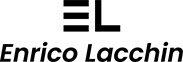
\includegraphics[width=0.3\columnwidth]{img/logo_black}}\lfoot{© Enrico Lacchin | \url{www.enricolacchin.com}}
\cfoot{}
\rfoot{\thepage}

\leftskip 0.0pt
\lstset{numbers=left, % vogliamo numerare le righr
  numberstyle=\tiny, % i numeri sono piccoli
  basicstyle=\ttfamily, % usiamo il carattere dattilografico
  columns=fullflexible, % niente emulazioni di allineamento
  backgroundcolor=\color{Snow2}%, % colore di sfondo
}

%----------------------------------------------
% INIZIO DOCUMENTO
%----------------------------------------------
\begin{document}

%----------------------------------------------
% TITOLO
%----------------------------------------------
\pagenumbering{gobble}

\small{Enrico Lacchin}

\MidSep
\textbf{\LARGE{Architetture dei sistemi digitali}}

\MidSep
\textit{\Large{Appunti}}
\Sep

\begin{center}

\includegraphics[width=1\columnwidth]{img/architetture.jpeg}
\end{center}

\vfill
Materia: Architetture dei sistemi digitali

Docente: Alberto Carini

Link moodle: \url{https://moodle2.units.it/course/view.php?id=9113}

%----------------------------------------------
% INDICE
%----------------------------------------------

\clearpage
\pagenumbering{roman}
\setcounter{page}{1}
\tableofcontents

%----------------------------------------------
% INIZIO CAPITOLI
%----------------------------------------------
%CAPITOLO 1
\clearpage

\pagenumbering{arabic}
\setcounter{page}{1}

\section{Computer Abstractions and Technology}
\subsection{Introduzione}
Negli ultimi decenni, ci sono stati numerosi nuovi computer la cui introduzione sembrava rivoluzionare l'industria informatica; queste rivoluzioni sono state interrotte solo perché qualcun altro ha costruito un computer ancora migliore.\\
Questa corsa all'innovazione ha portato a progressi senza precedenti dall'inizio dell'informatica alla fine degli anni '40.\\
\textsl{Se l'industria dei trasporti fosse stata al passo con quella dei computer, ad esempio, oggi potremmo viaggiare da New York a Londra in un secondo con un centesimo.}
Ogni volta che il costo dell'informatica aumenta di un altro fattore 10, le opportunità per i computer si moltiplicano. Le applicazioni che erano economicamente irrealizzabili diventano improvvisamente pratiche.
Nel recente passato, le seguenti applicazioni erano "fantascienza informatica":
\begin{itemize}
\item Computer nelle automobili
\item Cellulari
\item Sequenziamento del genoma umano
\item World Wide Web
\item Motori di ricerca
\end{itemize}

\subsection{Classi tradizionali di Computer}
I computer sono utilizzati in tre classi di applicazioni dissimili:\\
\paragraph{Personal computer (PC)} Un computer progettato per l'uso da parte di un individuo, generalmente dotato di un display grafico, una tastiera e un mouse.\\
\paragraph{Server} Un computer utilizzato per eseguire programmi più grandi per più utenti, spesso contemporaneamente, e
in genere si accede solo tramite una rete. Hanno alta capacità, prestazioni, affidabilità. Gamma da piccolo server alle dimensioni di un edificio. \textsl{Supercomputer}: Una classe di computer con le prestazioni e i costi più elevati; sono configurati come
server e in genere costano da decine a centinaia di milioni di dollari. Allo stato attuale consistono in decine di migliaia di processori con molti terabyte di memoria e rappresentano il vertice della capacità computazionale. Sono solitamente usati per complessi calcoli scientifici
e ingegneristici.\\
\paragraph{Embedded Computer}: Un computer all'interno di un altro dispositivo utilizzato per eseguire uno predeterminato
applicazione o raccolta di software. Applicazioni embedded spesso hanno requisiti unici che combinano minime performance con stringenti limitazioni su costi e potenza. Spesso i computer embedded hanno una tolleranza bassa a fallire, poiché i risultati possono essere devastanti (come il crash del computer di bordo di un aereo). \textsl{Per esempio: navigatore dell'auto, altimetro dell'aereo, smartwatch etc.}

\subsubsection{L'era PostPC}
\paragraph{Personal mobile devices (PMDs)} sono piccoli dispositivi wireless per la connessione a Internet; si basano sulle batterie per l'alimentazione e il software viene installato scaricando le app. Esempi convenzionali sono smartphone e tablet.\\
\paragraph{Cloud Computing} si riferisce a grandi raccolte di server (in giganteschi datacenter noti come Warehouse Scale Computers (WSC)) che forniscono servizi su Internet; alcuni provider affittano un numero di server variabile in modo dinamico come utilità.\\
\paragraph{Software as a Service (SaaS)} fornisce software e dati come servizio su Internet, di solito tramite un programma leggero come un browser che viene eseguito su dispositivi client locali, invece del codice binario che deve essere installato, e viene eseguito interamente su quel dispositivo. Gli esempi includono la ricerca sul web e i social network.

\subsection{Definizioni}
\begin{center}
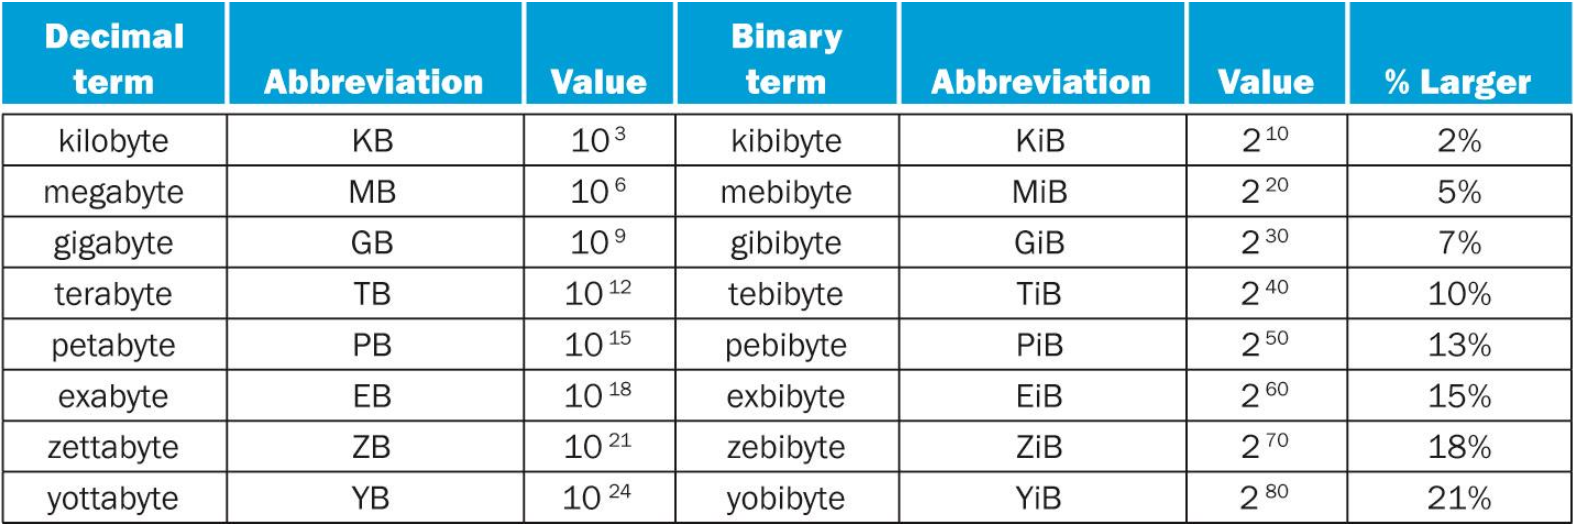
\includegraphics[width=1\columnwidth]{img/byte.png}
\end{center}

\subsection{Comprendere le performance di un programma}
Le performance di un programma dipendono da una combinazione dell'efficacia degli algoritmi usati nel programma, dei software utilizzati per creare e tradurre il programma in linguaggio macchina, e  del computer nell'eseguire queste istruzioni.
\begin{itemize}
	\item {\bfseries Algorithm:} determina sia il numero di istruzioni del codice e il numero di operazioni I/O da eseguire.
	\item {\bfseries Linguaggio di programmazione, compilatore e architettura:} determina il numero di istruzioni macchina per ogni istuzione del codice.
	\item {\bfseries Processore e memoria:} determina quanto velocemente le istruzioni possono essere eseguite.
	\item {\bfseries Sistemi di I/O:} determinano quanto velocemente le operazioni di I/O possono esssere eseguite.
\end{itemize}

\subsection{8 Grandi idee}
\begin{enumerate}
\item \textcolor{blue}{Progettare seguendo la legge di Moore}
\begin{itemize}
\item La legge di Moore afferma che le risorse del circuito integrato raddoppiano ogni 18-24 mesi.
\item Poiché i progetti di computer possono richiedere anni, le risorse disponibili per chip possono facilmente raddoppiare o raddoppiare quadruplicare tra l'inizio e la fine del progetto.
\item Gli ingegneri informatici devono anticipare dove sarà la tecnologia al termine del progetto piuttosto che progettare per dove inizia.
\end{itemize}
\clearpage
\item \textcolor{blue}{Utilizzare l'astratto per semplificare la progettazione}
\begin{itemize}
\item Una delle principali tecniche di produttività per hardware e software consiste nell'utilizzare le astrazioni per caratterizzare
il design a diversi livelli di rappresentazione; i dettagli di livello inferiore sono nascosti per offrire un modello più semplice ai livelli superiori.
\end{itemize}
\item \textcolor{blue}{Rendere il caso comune veloce}
\begin{itemize}
\item Rendere veloce il caso comune tenderà a migliorare le prestazioni meglio rispetto all'ottimizzazione del caso raro. Spesso il caso più comune è anche quello più semplice e quindi anche quello più facile da migliorare.
\end{itemize}
\item \textcolor{blue}{Performance tramite parallelismo}
\begin{itemize}
\item Fin dagli albori dell'informatica, gli ingegneri informatici hanno offerto progetti che ottengono di più prestazioni mediante operazioni di calcolo in parallelo.
\end{itemize}
\item \textcolor{blue}{Performance tramite piepline}
\begin{itemize}
\item Un particolare modello di parallelismo.
\item Divide le operazioni in piccole fasi, ad es. fetch, decode, execute. Mentre l'istruzione $i$ viene eseguita, $i+1$
viene decodificata, $i+2$ viene recuperata.
\end{itemize}
\item \textcolor{blue}{Performance tramite predizioni}
\begin{itemize}
\item Può essere in media più veloce indovinare il caso in cui ci si trova per iniziare a lavorarci subito, piuttosto che aspettare fino a quando non lo si sa con certezza, a patto che il meccanismo per rimediare da una previsione errata non sia troppo costoso e che la previsione sia relativamente accurata.
\end{itemize}
\item \textcolor{blue}{Gerarchie di memoria}
\begin{itemize}
\item I programmatori vogliono che la memoria sia veloce, grande ed economica, poiché la velocità della memoria spesso modella prestazioni, la capacità limita la dimensione dei problemi che possono essere risolti e il costo della memoria oggi è spesso la maggior parte del costo del computer.
\item Possiamo affrontare queste richieste contrastanti con una gerarchia di memoria, con la memoria più veloce, più piccola e più costosa per bit in cima alla gerarchia e la più lenta, più grande e più economica per bit in fondo.
\item Le cache danno l'illusione che la memoria principale sia veloce quasi quanto la cima della gerarchia e grande ed economico quasi quanto il fondo della gerarchia.
\begin{center}
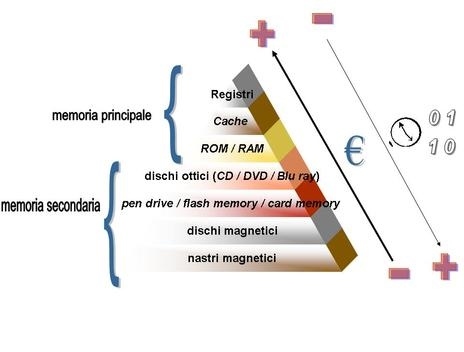
\includegraphics[width=0.6\columnwidth]{img/piramide_memorie.jpeg}
\end{center}
\end{itemize}
\item \textcolor{blue}{Affidabilità tramite ridondanza}
\begin{itemize}
\item I computer non solo devono essere veloci; devono essere affidabili.
\item Poiché qualsiasi dispositivo fisico può guastarsi, rendiamo i sistemi affidabili includendo componenti ridondanti che possono subentrare quando si verifica un errore e per aiutare a rilevare i guasti.
\end{itemize}
\end{enumerate}

\subsection{Al di sotto del programma}
\begin{center}
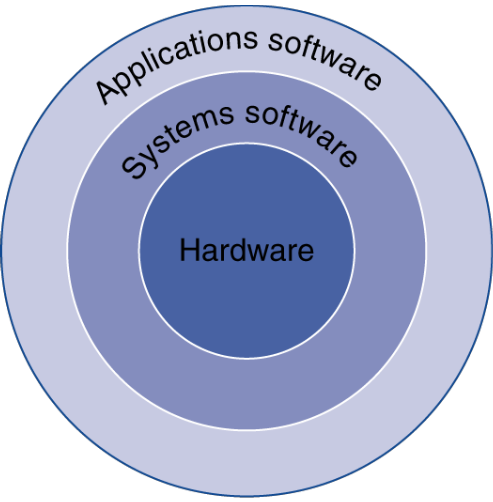
\includegraphics[width=0.4\columnwidth]{img/programma.png}
\end{center}
Per passare da una complessa applicazione alle istruzioni primitive ci sono diversi livelli di software che interpretano e traducono operazioni di alto livello in semplici istruzioni macchina. Questi strati si software sono organizzati in modo gerarchico con le applicazioni come anello più esterno e diversi software di sistema posti tra l'hardware fisico e il programma applicativo.
\begin{itemize}
\item \textbf{Application Software}: tutte le milioni di righe di codice del programma scritte in un linguaggio di programmazione ad alto livello (C, java, etc.).
\item \textbf{System Software}: Software che fornisce servizi comunemente utili, inclusi sistemi operativi, compiler, loaders e assemblers. Ci sono diversi tipi di programmi di sistema ma i principali sono il compilatore e il sistema operativo.\\
\textsl{Compilatore}: converte il codice ad alto livello (HLL) in codice macchina.\\
\textsl{Sistema Operativo}: Programma di supervisione che gestisce le risorse di un computer a vantaggio dei programmi che vengono eseguiti su quel computer:
\begin{itemize}
\item Gestione input/output
\item Gestione della memoria e dell'archiviazione
\item Pianificazione delle attività e condivisione delle risorse
\end{itemize}
\item \textbf{Hardware}: Tutte le componenti materiali, processore, memoria, sistemi di I/O
\end{itemize}

\subsection{Da un linguaggio ad alto livello al linguaggio hardware}
Un \textcolor{blue}{istruzione} è un comando che gli hardware dei computer capiscono e al quale obbediscono. Le istruzioni sono collezioni di bits e possono essere pensate come numeri.\\
Un \textcolor{blue}{assembler} è un programma che traduce una versione simbolica di istruzioni (assembly language) nella versione in codice binario (machine language).\\
L'\textcolor{blue}{assembly language} è una rappresentazione simbolica delle istruzioni macchina.\\
Il \textcolor{blue}{machine language} è la rappresentazione binaria delle istruzioni macchina.\\
\\
Un \textcolor{blue}{linguaggio ad alto livello} è il livello di astrazione più vicino al linguaggio "quotidiano". Fornisce produttività e portabilità: \begin{itemize}
	\item permettono al programmatore di pensare in un linguaggio molto più naturale
	\item la velocità nel programmare aumenta perché un'idea la si esprime in meno linee di codice
	\item i programmi diventano indipendenti dalla macchina in cui verrano utilizzati, perché i compilatori e gli assembler possono tradurre un linguaggio di alto livello nelle istruzioni macchina di qualsiasi computer
\end{itemize}
Il \textcolor{blue}{linguaggio assembly} è una rappresentazione testuale delle istruzioni.\\
La \textcolor{blue}{rappresentazione hardware} è composta solamente da cifre binarie (bit) e le istruzioni e i dati sono codificati.
\begin{center}
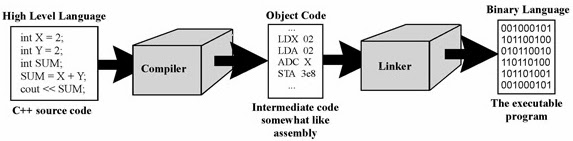
\includegraphics[width=1\columnwidth]{img/HLL_to_machine.jpeg}
\end{center}

\subsection{Componenti di un computer}
I 5 componenti classici di un computer sono \textsl{input}, \textsl{output}, \textsl{memoria}, \textsl{datapath} e \textsl{control}, con gli ultimi due a volte combinati e chiamati processore o central processing unit (CPU). Questa organizzazione è indipendente dalla tecnologia hardware: puoi inserire ogni pezzo di ogni computer, passato e presente, in una di queste cinque categorie.
\begin{center}
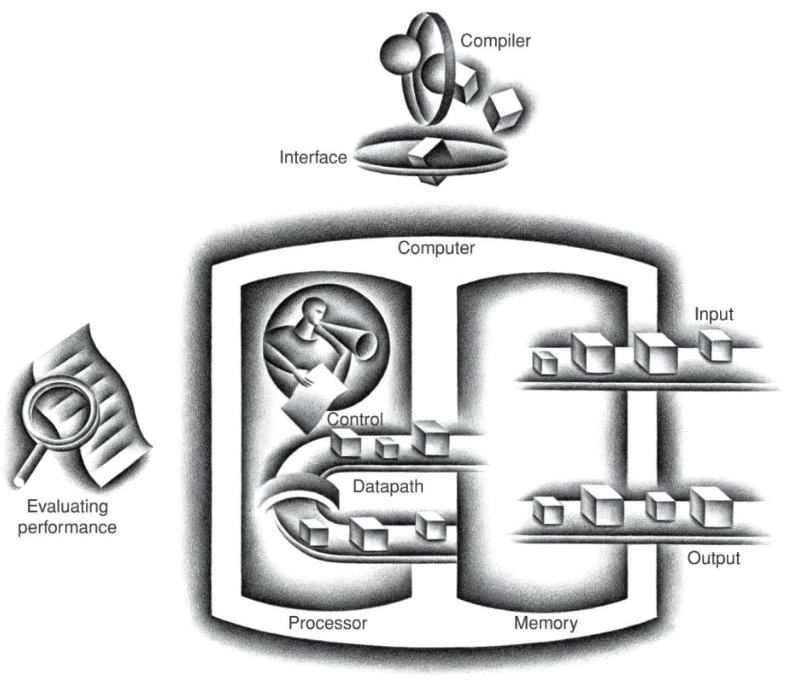
\includegraphics[width=0.6\columnwidth]{img/computer_component.png}
\end{center}
La central processing unit (CPU) viene anche chiamato processore. \'E la parte attiva del computer, che contiene il datapath e il control e che svolge operazioni aritmetiche, segnala l'attivazione dei dispositivi I/O e così via.

\subsubsection{Processore (CPU)}
\textbf{Datapath}: la componente del processore che svolge le operazioni aritmetiche.\\
\textbf{Control}: la componente del processore che comanda il datapath, la memoria e i dispositivi di I/O in accordo alle istruzioni date dal programma in esecuzione.

\subsubsection{Memoria}
La memoria è l'area di archiviazione in cui vengono conservati i programmi quando sono in esecuzione e che contiene i dati necessari per i programmi in esecuzione.\\
Esistono diversi tipi di memoria:
\begin{itemize}
\item \textbf{Dynamic Random Access Memory (DRAM)}: memoria costruita come circuito integrato; fornisce un accesso casuale a qualsiasi posizione. I tempi di accesso sono 50 nanosecondi circa
\item \textbf{Static Random Access Memory (SRAM)}: memoria costruita come un circuito integrato, ma più veloce e meno densa della DRAM.
\item \textbf{Memoria cache}: una memoria piccola e veloce che funge da buffer per una memoria più lenta e più grande. Tipicamente SRAM.
\end{itemize}
SRAM e DRAM sono memorie volatili: vengono utilizzate per contenere dati e programmi mentre sono in esecuzione; ma abbiamo bisogno di memoria non volatile utilizzata per archiviare programmi e dati tra le esecuzioni.\\

\paragraph{Memoria primaria e secondaria}

Andremo a distinguere la memoria in \textsl{main memory} (o memoria primaria) e \textsl{secondary memory}.\\
\begin{itemize}
\item \textbf{Main memory}: memoria utilizzata per contenere i programmi mentre sono
in esecuzione; in genere, nei computer odierni, è costituita da DRAM.
\item \textbf{Secondary memory}: memoria non volatile utilizzata per memorizzare programmi e dati tra un'esecuzione e l'altra; in genere è costituita da memorie flash nei PMDs (Personal Mobile Devices), SSDs (Solide State Disks) e dischi magnetici (Hard Disk) nei server.
\end{itemize}
\textcolor{blue}{Disco magnetico}: detto anche Hard Disk. Una forma di memoria secondaria non volatile composta da piatti rotanti rivestiti con un materiale di registrazione magnetico. Poiché sono dispositivi meccanici rotanti, i tempi di accesso sono compresi tra 5 e 20 millisecondi.\\
\textcolor{blue}{Memoria flash}: una memoria a semiconduttore non volatile. È più economico e più lento della DRAM ma più costoso per bit e più veloce dei dischi magnetici. I tempi di  accesso sono di circa 5-50 microsecondi.

\subsection{Astrazioni}
Una delle astrazioni più importanti è l'interfaccia tra l'hardware e il software di livello più basso: l'\textcolor{blue}{architettura del set di istruzioni (ISA - Instruction set architecture)}, o semplicemente architettura, di un computer. L'architettura del set di istruzioni include tutto ciò che i programmatori devono sapere per far funzionare correttamente un programma in linguaggio macchina binario, incluse istruzioni, dispositivi I/O e così via. In genere, il sistema operativo incapsula i dettagli dell'esecuzione dell'I/O, dell'allocazione della memoria e di altre funzioni di sistema di basso livello.\\
\textcolor{blue}{Interfaccia binaria dell'applicazione (ABI - Application binary interface)}: definisce l'interfaccia tra il sistema operativo e le proprie applicazioni a livello di linguaggio macchina. La parte utente del set di istruzioni più l' interfaccia del sistema operativo utilizzate dai programmatori dell'applicazione (ISA + interfaccia software di sistema). Definisce uno standard per la portabilità binaria tra computer.\\
Si noti che distinguiamo l'architettura del set di istruzioni da un'\textsl{implementazione} dell'architettura: un'implementazione è un hardware che obbedisce all'astrazione dell'architettura. Questa interfaccia astratta consente a molte implementazioni di costi e prestazioni variabili di eseguire software identico.

\subsection{Tecnologie per costruire processori e memorie}
La manifattura di un \textcolor{blue}{circuito integrato} (o \textcolor{blue}{chip}) inizia con il siliceo, una sostanza che non conduce bene l'elettricità essendo un semiconduttore. Con particolari processi chimici è possibile aggiungere materiali al siliceo che permettono a piccole porzioni di trasformarsi o in eccellenti conduttori, o in eccellenti isolanti o in aree che possono comportarsi sia da conduttori che da isolanti sotto specifiche condizioni. Il processo inizia da un lingotto di cristallo di silicio che viene finemente tagliato in \textcolor{blue}{wafers}. I wafer subiscono poi una serie di processi chimici che creano i transistor, porzioni conduttori e isolanti. Piccole imperfezioni nel wafer possono compromettere il suo funzionamento e per questo un unico wafer è composto da chip indipendenti (detti dies) che vengono separati e testati, in modo che i chip difettati vengano scartati.
\begin{center}
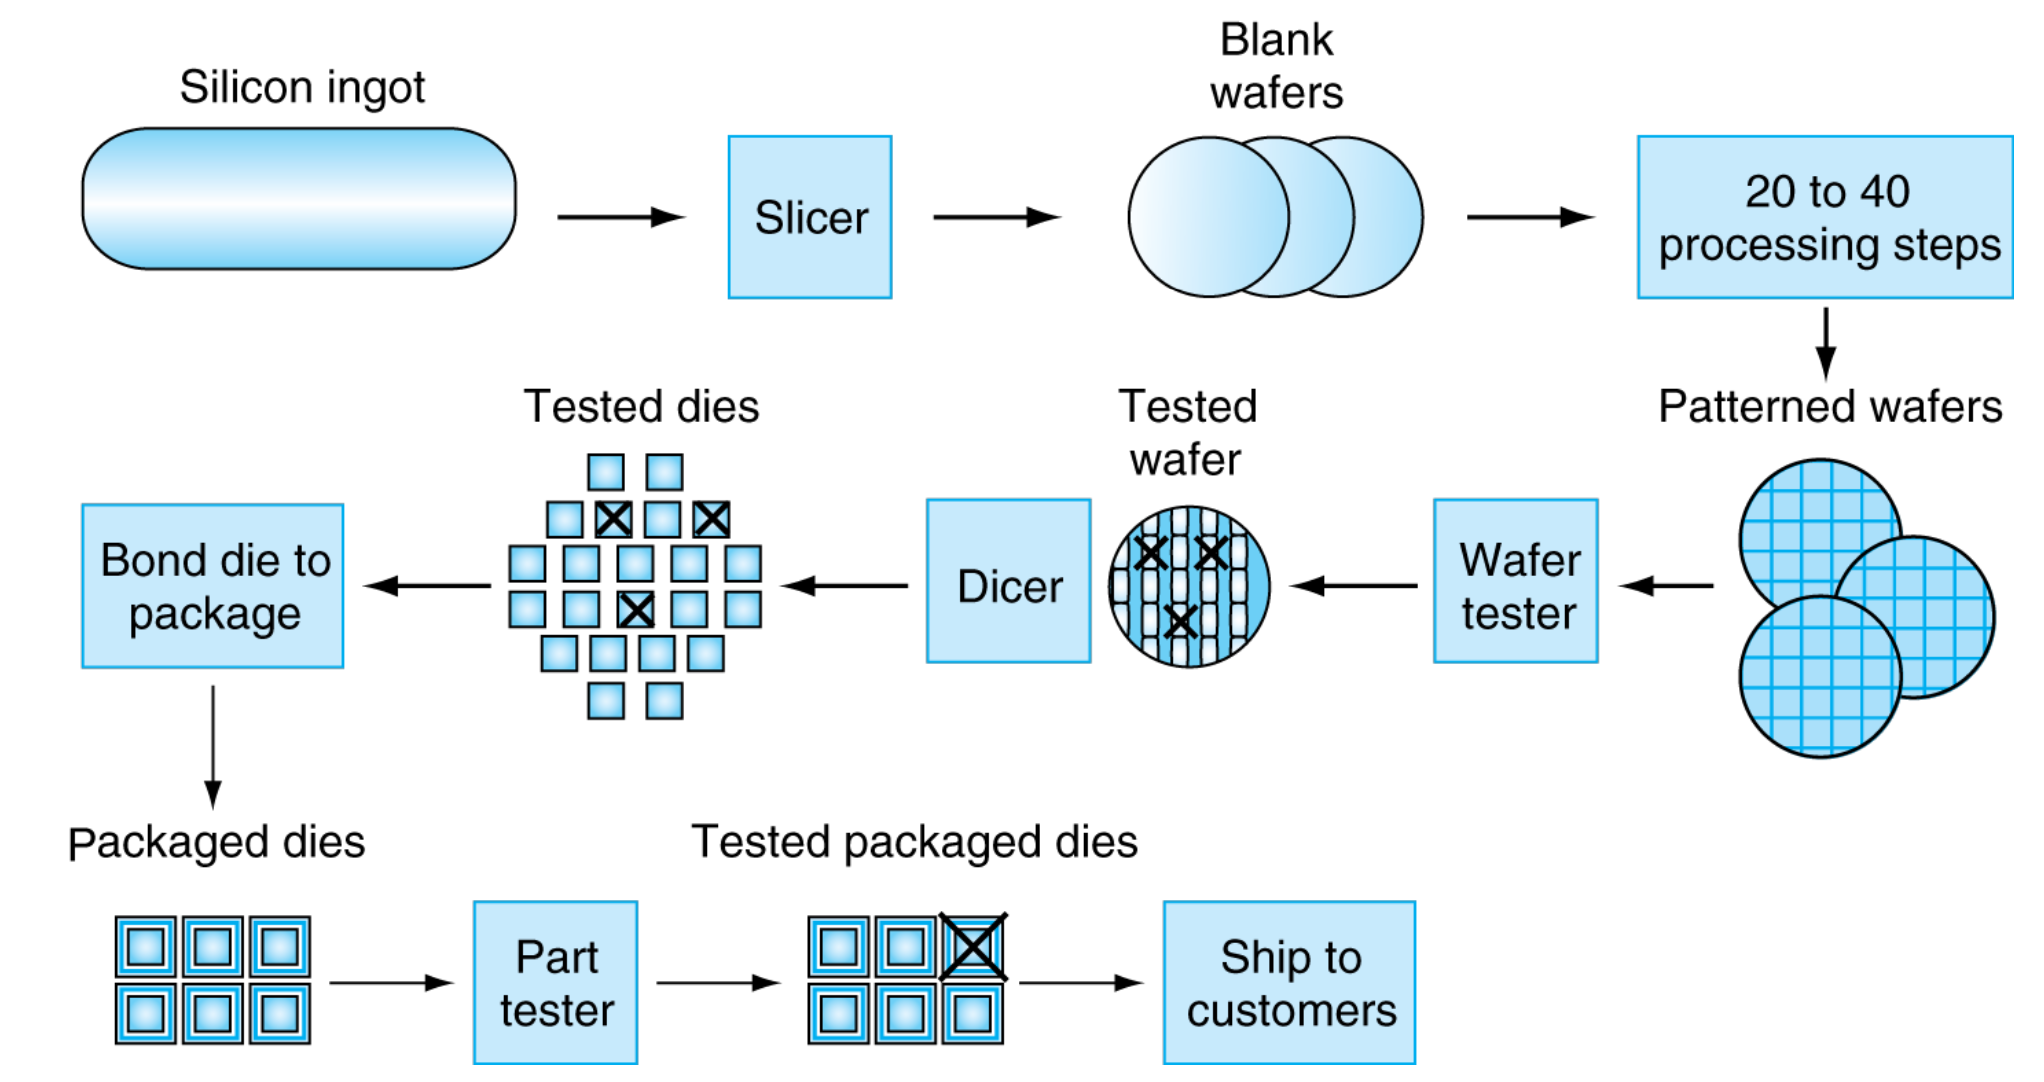
\includegraphics[width=0.7\columnwidth]{img/processor_building.png}
\end{center}
\textbf{Yield (rendimento)}: la percentuale di piastre buone rispetto al numero totale di chip (dies) sul wafer.
$$Costo\ chip = {Costo\ wafer \over Chip\ sul \ wafer \times Yield}$$
$$Chip\ sul\ wafer \approx {Area\ wafer \over Area\ chip}$$
$$Yield = {1\over \left[1+\left(Difetti\ per\ area \times {Area\ chip \over 2}\right)\right]^2}$$
La seconda equazione è un'approssimazione perché non tiene conto di dover sottrarre l'area vicino al bordo circolare del wafer che taglia parte di alcuni chip.
Non c'è una relazione lineare con area e tasso di difetto. Il costo e l'area del wafer sono fissi, il tasso di difetto è determinato dal processo di fabbricazione e l'area del singolo chip è determinata dall'architettura e dalla progettazione dei circuiti.

\subsection{Performance}
Quando diciamo che un computer ha prestazioni migliori di un altro, cosa intendiamo?
Quale dei seguenti aeroplani ha le migliori prestazioni?
Prima bisogna definire cosa si intende per prestazione, infatti si possono misurare in modo diverso le performance.
\begin{center}
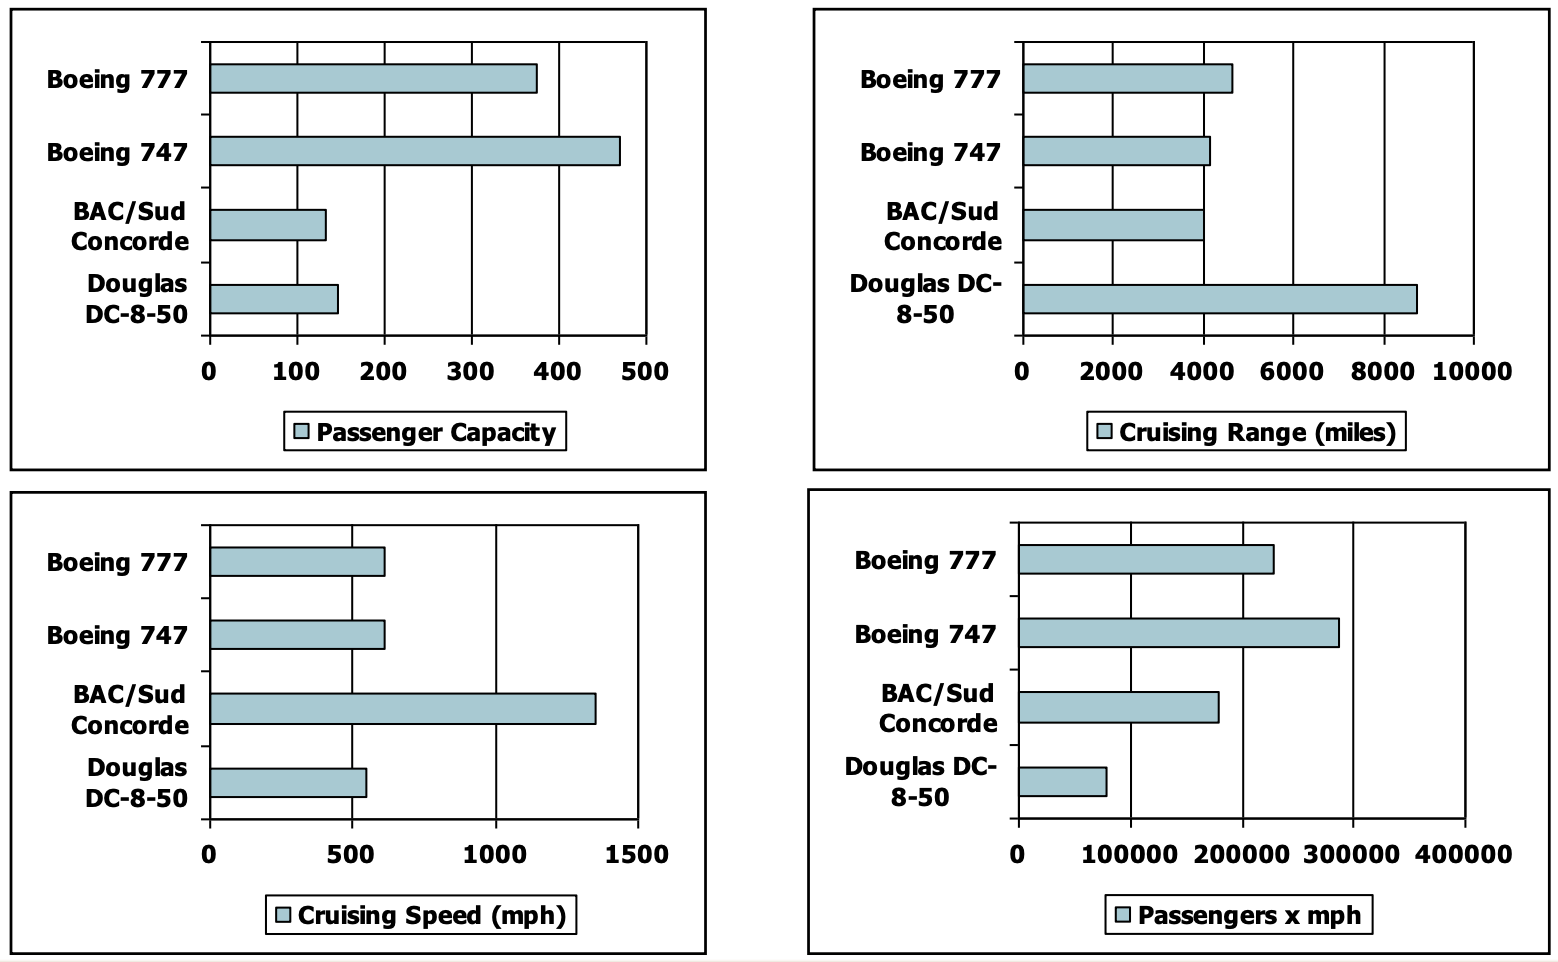
\includegraphics[width=0.7\columnwidth]{img/performance_plane.png}
\end{center}
\subsubsection{Tempo di risposta e Produttività}
Se stai eseguendo un programma su due diversi computer desktop, diresti che quello più veloce è il computer desktop che esegue il lavoro per primo. Se stai eseguendo un data center con diversi server che eseguono lavori inviati da molti utenti, diresti che il computer più veloce è stato quello che ha completato il maggior numero di lavori durante la giornata.\\
Il \textcolor{blue}{Response time} anche chiamato \textsl{execution time} è il tempo totale richiesto dal computer per completare un'attività, inclusi gli accessi al disco e alla memoria, le attività di I/O, l'effetto del sovraccarico del sistema operativo, il tempo di esecuzione della CPU e così via.\\
Il \textcolor{blue}{throughput} anche detto \textsl{bandwidth} è un'altra misura delle prestazioni: è il numero di attività completate per unità di tempo.\\
\\
In che modo vengono influenzati l'execution time e il throughput? Sostituendo il processore con una versione più veloce? Aggiungendo più processori?

\subsubsection{Performance relative}
Definiamo la performance come: $$Performance_X = {1 \over Execution\ time_X}$$
Con due computer $Performance_X > Performance_Y$ che equivale a scrivere $ Execution\ time_Y > Execution\ time_X$\\
Posso dire che $X$ è $n$ volte più veloce di $Y$ se $${Performance_X \over Performance_Y} = {Execution\ time_Y \over Execution\ time_X} = n$$

\subsubsection{Misurare le Performance}
Il tempo è la misura delle prestazioni del computer: il computer che esegue la stessa quantità di lavoro nel minor tempo è il più veloce. Tuttavia, il tempo può essere definito in modi diversi, a seconda di ciò che contiamo. La più semplice definizione di tempo è chiamata \textcolor{blue}{wall clock}, \textcolor{blue}{response time} o \textcolor{blue}{elapsed time}. Con questi termini definiamo il tempo totale per completare un'attività, inclusi accessi al disco, accessi alla memoria, attività di input/output (I/O), sovraccarico del sistema operativo: tutto.\\
Tuttavia i computer spesso sono condivisi e un processore potrebbe lavorare su diversi programmi simultanemente. In questi casi il sistema potrebbe provare a ottimizzare il throughtput piuttosto che provare a minimizzare il tempo trascorso su un dato programma. Il \textcolor{blue}{CPU execution time} anche detto \textsl{CPU time} è il tempo effettivo impiegato dalla CPU per l'elaborazione di un'attività specifica. Non include il tempo trascorso in attesa di I/O o nell'esecuzione di altri programmi. Il tempo della CPU può essere ulteriormente suddiviso in
\begin{itemize}
\item \textbf{user CPU time}: il tempo CPU impiegato nel programma stesso.
\item \textbf{system CPU time}: il tempo della CPU impiegato nel sistema operativo per eseguire attività per conto del programma.
\end{itemize}
Programmi diversi sono influenzati in modo diverso dalle prestazioni della CPU e del sistema.

\subsubsection{CPU Clocking}
Tutti i computer sono costruiti utilizzando un clock che determina quando si verificano eventi nell'hardware. Il periodo di clock (\textcolor{blue}{clock period}) è il tempo per un ciclo di clock completo (ad es. 250 picosecondi o 250 ps). La frequenza di clock (\textcolor{blue}{clock rate}) è l'inverso del periodo di clock (ad es. 4 gigahertz o 4 GHz).
Una semplice formula mette in relazione i cicli di clock e il tempo di ciclo di clock con il tempo della CPU:
$$CPU\ execution\ time\ = CPU\ clock\ cycles\ \times \ Clock\ cycle\ time$$
$$CPU\ execution\ time\ = {CPU\ clock\ cycles \over Clock\ rate}$$
Questa formula chiarisce che il progettista hardware può migliorare le prestazioni riducendo il numero di cicli di clock richiesti per un programma o la durata del ciclo di clock. Il progettista hardware deve spesso rinunciare a una maggiore frequenza di clock per ridurre i cicli necessari a un programma.

\subsubsection{Performance delle istruzioni}
Le precedenti equazioni delle prestazioni non includevano alcun riferimento al numero di istruzioni necessarie per il programma. Tuttavia visto che il computer deve eseguire le istruzioni generate dal compilatore, il tempo di esecuzione deve dipendere dal numero di istruzioni in un programma. Un modo per pensare al tempo di esecuzione è che sia uguale al numero di istruzioni eseguite moltiplicato per il tempo medio per istruzione.
$$CPU\ clock\ cycles = Instructions\ for\ a\ program\ \times Avg.\ clock\ cycles\ per\ instruction$$
\textcolor{blue}{Clock cycles per instruction (CPI)}: numero medio di cicli di clock per istruzione per un programma o un frammento di programma. Poiché istruzioni diverse possono richiedere tempi diversi a seconda di ciò che fanno, CPI è una media di tutte le istruzioni eseguite nel programma.

\subsubsection{CPU Performance - Equazione classica}
Ora possiamo scrivere l'equazione base delle performance in termini di numero di istruzioni, CPI e tempo del ciclo di clock ottenendo:
$$CPU \ time\ = \ Instruction\ count\ \times \ CPI \ \times \ Clock cycle time$$
o in termini di frequenza
$$CPU \ time\ = \ {Instruction\ count\ \times \ CPI \over Clock\ rate}$$

\subsubsection{CPI nel dettaglio}
Se classi di istruzioni diverse richiedono un numero di cicli diverso abbiamo che $$Clock\ cycles = \sum_{i=1}^n(CPI_i\ \times \ Instruction\ Count_i)$$
Media pesata del CPI: $$CPI = {Clock\ Cycles \over Instruction\ Count} = \sum_{i=1}^n\left(CPI_i\ \times \ {Instruction\ Count_i \over Instruction\ Count}\right)$$ dove definiamo ${Instruction\ Count_i \over Instruction\ Count}$ come frequenza relativa.

\subsubsection{Riassunto}
$$Time = Seconds / Program = {Instructions \over Program} \times {Clock\ cycles \over Instruction} \times {Seconds \over Clock \ cycle}$$
Le performance di un programma dipendono da:
\begin{itemize}
\item \textbf{Algoritmo}: determina il numero di istruzioni del programma sorgente eseguite e quindi il numero di istruzioni del processore eseguite. Può anche influenzare il CPI favorendo istruzioni più lente o più veloci.
\item \textbf{Linguaggio di programmazione}: influisce sul conteggio delle istruzioni, poiché le istruzioni da un certo linguaggio vengono tradotte in istruzioni macchina, che determinano il conteggio delle istruzioni. Può anche influenzare il CPI a causa delle sue caratteristiche. Per esempio un forte supporto per l'astrazione dei dati richiede chiamate indirette, che utilizzano istruzioni CPI più elevate.
\item \textbf{Compilatore}: influisce sia sul conteggio delle istruzioni che sui cicli medi per istruzione, poiché determina la
traduzione delle istruzioni dal linguaggio di partenza a istruzioni per il computer.
\item \textbf{ISA}: influisce su tutti e tre gli aspetti delle prestazioni della CPU, poiché influisce sulle istruzioni necessarie per una
funzione, il numero di cicli per ciascuna istruzione e la frequenza di clock complessiva del processore.
\end{itemize}

\subsection{The power wall}
La tabella mostra l'aumentare della frequenza di clock e potenza di microprocessori Intel nell'arco di trent'anni. La ragione per cui crescono assieme è che sono correlati, e il motivo per il loro rallentamento è dovuto al raggiungimento del limite di potenza per rafreddare i microprocessori.
\begin{center}
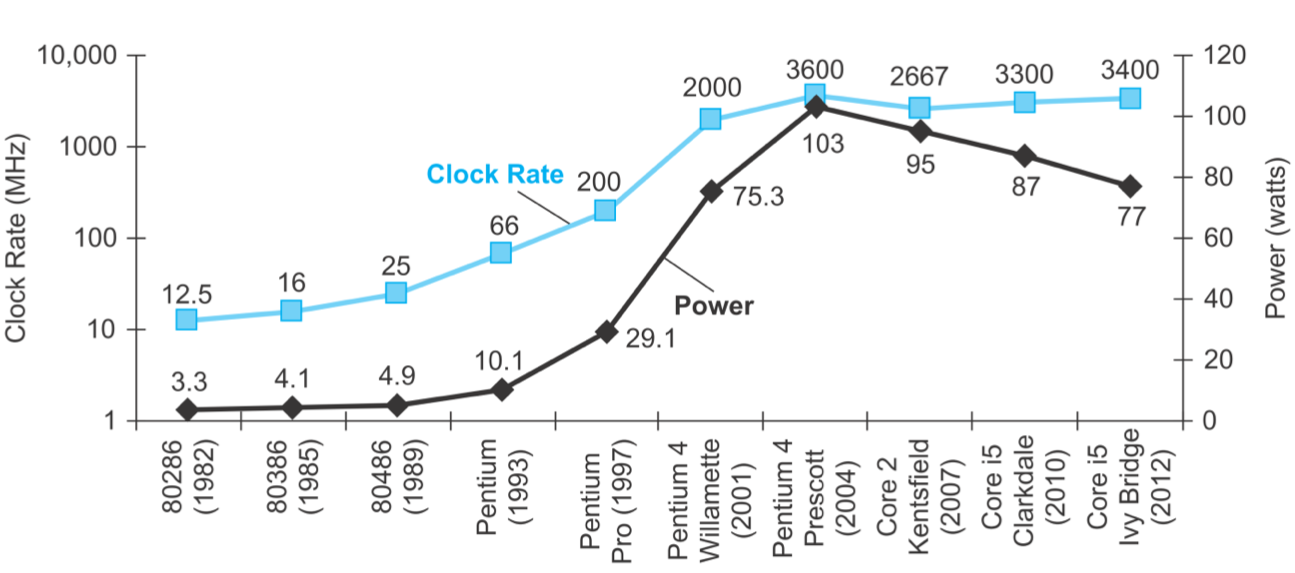
\includegraphics[width=0.8\columnwidth]{img/powerwall.png}
\end{center}
\subsubsection{Dissipazione di potenza in CMOS}
Nei CMOS (Complementary Metal-Oxide Semiconductor) la fonte primaria di consumo di energia è la cosiddetta energia dinamica, ovvero l'energia che viene consumata quando i gate cambiano stato da 0 a 1 e viceversa.\\
Per la transizione $0 \rightarrow 1 \rightarrow 0$ o $1 \rightarrow 0 \rightarrow 1$: $$Energy\ \propto\ Capacitive\ load \ \times \ Voltage^2$$
Per una singola transizione $0 \rightarrow 1$ oppure $1 \rightarrow 0$ $$Energy\ \propto\ {1\over2}\times \ Capacitive\ load \ \times \ Voltage^2$$
La potenza richiesta per porta è semplicemente il prodotto dell'energia di una transizione e la frequenza delle transizioni, che dipende dalla frequenza di clock:
$$Power\ \propto\ {1\over2}\times \ Capacitive\ load \ \times \ Voltage^2 \ \times\ Frequency\ switched$$
Come possono le frequenze di clock crescere di un fattore 1000 mentre la potenza è aumentata solo di un fattore 30?
Energia e potenza sono state ridotte abbassando la tensione, che si verificava ad ogni nuova generazione di tecnologia, passando da 5V fino a valori inferiori a 1V.

\subsubsection{Problemi moderni nella dissipazione dell'energia}
Il problema moderno è che un ulteriore abbassamento della tensione sembra rendere i transistor poco affidabili per via delle correnti parassite (leakage current). Sebbene l'energia dinamica sia la principale fonte di consumo di energia nei CMOS, il consumo di energia statica si verifica a causa della corrente di dispersione che scorre anche quando un transistor è spento. Nei server, le perdite sono in genere responsabili del 40\% del consumo energetico.\\
Aumentando il numero di transistor si aumenta la dissipazione di potenza, anche se i transistor sono sempre spenti. Una varietà di tecniche di progettazione e innovazioni tecnologiche vengono implementate per controllare le perdite, ma
è difficile abbassare ulteriormente la tensione.

\subsection{Multiprocessori}
I microprocessori multicore posseggono più di un processore per chip e offrono vantaggi maggiori sul numero di operazioni per unità di tempo (throughput) che sui tempi di risposta. La tecnica della \textcolor{blue}{pipeline} permette di velocizzare l'esecuzione dei programmi facendo eseguire più operazioni in contemporanea, un esempio di \textit{instruction-level parallelism} dove la natura parallela dell'hardware viene astratta, così che il programmatore può pensare all'hardware come se eseguisse le operazioni in modo sequenziale. \\
\'E però richiesta una programmazione esplicitamente parallela e più complessa. La velocità in un hardware con parallelismo dipende da come si divide il carico di lavori nei vari processori (cores) e che le operazioni ulteriori dovute alla pianificazione e alla cordinazione per il parallelismo non sprechi la capacità di calcolo aggiuntiva.\\
Per i programmatori è complicato:\begin{itemize}
\item Massimizzare le performance
\item Bilanciare il carico dei processori
\item Ottimizzare la comunicazione e la sincronizzazione
\end{itemize}

\subsection{SPEC CPU Benchmark}
Le prestazioni dei processori vengono misurate utilizzando programmi di benchmark che rappresentano presumibilmente tipici carichi di lavoro effettivi.\\
SPEC (System Performance Evaluation Cooperative) è uno sforzo finanziato e supportato da numerosi fornitori di computer per creare serie standard di benchmark per i moderni sistemi informatici. Sviluppa benchmark per CPU, I/O, Web, \dots \\
SPEC CPU2006 è costituito da una serie di 12 benchmark interi (CINT2006) e 17 a virgola mobile (CFP2006). Va a vedere:
\begin{itemize}
\item Tempo trascorso per eseguire una selezione di programmi
\item I/O trascurabile, quindi si concentra sulle prestazioni della CPU
\item Normalizza rispetto alla macchina di riferimento
\item Riassumere come media geometrica dei rapporti di prestazione
$$\sqrt[n]{\prod_{i=1}^n Execution\ time\ ratio_i}$$
\end{itemize}

\subsection{SPEC Power Benchmark}
Segnala il consumo energetico dei server a diversi livelli di carico di lavoro, suddiviso in incrementi del 10\%, in un periodo di tempo.\\
SPECpower iniziava con un altro benchmark SPEC per le applicazioni aziendali Java che sforzava i processori, cache, memoria principale, Java virtual machine, compilatore, garbage collector e parti del sistema operativo.\\
Le prestazioni sono misurate in throughput, come numero di operazioni al secondo. I risultati dei singoli test sono poi fusi in un unico numero chiamato "overall ssj\_ops per watt":
\begin{displaymath}
	overall\ ssj\_ops\ per\ watt = \frac{\displaystyle\sum_{i=0}^{10}ssj\_ops_i}{\displaystyle\sum_{i=0}^{10} power_i}
\end{displaymath}
Dove $ssj\_ops_i$ è la performance ad ogni incremento del 10\% e $power_i$ è la potenza consumata ad ogni livello di prestazione.

\subsection{Errore: Bassa potenza al minimo}
\begin{center}
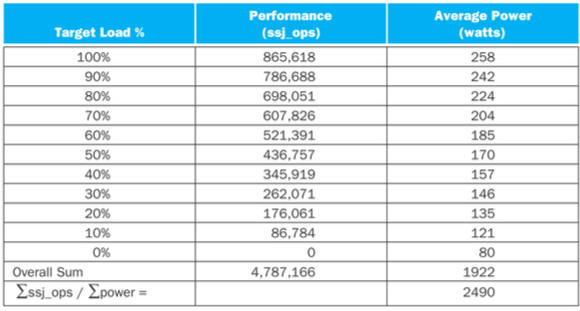
\includegraphics[width=0.9\columnwidth]{img/xeon.png}
\end{center}
Guardando il benchmark dello Xeon X5650 notiamo che:
\begin{itemize}
\item Al 100\% di carico consuma 258 W
\item Al 50\% di carico consuma 170 W (66\%)
\item Al 10\% di carico consuma 121 W (47\%)
\end{itemize}
Dovremmo progettare hardware per ottenere una "capacità di calcolo proporzionale all'energia". Se i server futuri utilizzassero, ad esempio, il 10\% della potenza di picco al 10\% del carico di lavoro, potremmo ridurre la bolletta dell'elettricità di datacenter ed emissioni di $CO_2$.

\subsection{Insidia: Legge di Amdahl}
Un'insidia comune: migliorare un aspetto di un computer e aspettarsi un miglioramento proporzionale delle prestazioni complessive.\\
La legge di Amdahl afferma che il tempo di esecuzione del programma dopo aver apportato il miglioramento è
$$T_{improved} = {T_{affected} \over improvement\ factor}+ T_{uneffected}$$

\subsection{Fallacia: Computers at low utilization use little power}
L'efficienza a bassi carichi di utilizzo è importante. Ad esempio i server WSC della Google lavorano tra il 10\% e il 50\% il più del tempo e al 100\% per meno dell'1\% del tempo.

\subsection{Insidia: MIPS come metrica delle performance}
Un comune errore è valutare le performance utilizzando solo uno o due dei parametri (periodo di clock, numero di istruzioni e CPI). L'analisi con 2 dei tre fattori può essere valida solo in limitati contesti.\\
Un alternativa all'uso del tempo sono i \textbf{MIPS}: Millions of Instructions Per Second. Dato un programma:\\
$$MIPS = {Instruction\ count \over Execution\ time \times 10^6} = {Instruction\ count \over {Instruction\ count \times CPI \over Clock\ rate} \times 10^6} = {Clock\ rate \over CPI \times 10^6}$$
Non tiene conto delle differenze negli ISA tra computer e delle differenze di complessità tra le istruzioni. Sostituendo il tempo di esecuzione si osserva la relazione tra MIPS e CPI, quest ultimo varia tra i programmi su una determinata CPU e quindi lo stesso vale per il MIPS.

%CAPITOLO 2
\clearpage
\section{Instructions: Language of the Computer}
\subsection{Introduzione}
Per comandare l'hardware di un computer, devi parlarne la sua lingua. Le parole della lingua di un computer sono chiamate istruzioni e il suo vocabolario è chiamato set di istruzioni. I linguaggi informatici sono abbastanza simili, più simili ai dialetti regionali che alle lingue indipendenti.\\
Il set di istruzioni scelto è ARMv8, introdotto nel 2011. Useremo un sottoinsieme di ARMv8, chiamato LEGv8  ("Lessen Extrinsic Garrulity"). Questa somiglianza dei set di istruzioni si verifica perché:
\begin{itemize}
\item Tutti i computer sono costruiti sulla base di principi di base simili
\item Ci sono alcune operazioni di base che tutti i computer devono fornire
\item I progettisti di computer hanno un obiettivo comune: il linguaggio dovrebbe facilitare la costruzione del file hardware e il compilatore massimizzando le prestazioni e riducendo al minimo i costi e l'energia.
\end{itemize}

\subsection{Operazioni dell'Hardware dei Computer}
Ogni computer deve essere in grado di eseguire operazioni aritmetiche. La notazione LEGv8 per sommare le due variabili b e c e per mettere la loro somma in a è 
\begin{center}
\begin{minipage}{.2\linewidth}
\begin{verbatim}
ADD a, b, c
\end{verbatim}
\end{minipage}
\end{center}
Tutte le operazioni aritmetiche hanno questa forma. Supponiamo di voler inserire la somma di quattro variabili b, c, d ed e nella variabile a:
\begin{verbatim}
ADD a, b, c // La somma di b e c viene messa in a
ADD a, a, d // La somma di b, c e d è ora in a
ADD a, a, e // La somma di b, c, d ed e è ora in a
\end{verbatim}
Richiedere che ogni istruzione abbia esattamente tre operandi è conforme alla filosofia di mantenere l'hardware semplice: hardware per un numero variabile di operandi è più complicato che per un numero fisso.\\
\begin{center}\textcolor{red}{\textbf{Primo principio di progettazione}: La semplicità favorisce la regolarità}\end{center}

\subsubsection{Compilare un codice C in LEGv8}
Codice C: 
\begin{center}
\begin{minipage}{.2\linewidth}
\begin{verbatim}
f = (g+h) - (i+j);
\end{verbatim}
\end{minipage}
\end{center}
Cosa andrà a produrre il compilatore?
\begin{verbatim}
ADD t0, g, h // Variabile temporanea t0 che contiene g + h
ADD t1, i, j // Variabile temporanea t1 che contiene i + j
SUB f, t0, t1 // f data da t0 - t1, che equivale a dire (g + h)- (i + j)
\end{verbatim}

\subsection{Operandi dell'Hardware dei Computer}
Le istruzioni aritmetiche utilizzano operandi di registro. LEGv8 ha un file di registro a 32 $\times$ 64-bit utilizzati per i dati a cui si accede di frequente.
\begin{itemize}
\item 64-bit data vengono chiamati "doubleword". 31 $\times$ 64-bit per uso generico utilizzano registri "X" da X0 a X30
\item 32-bit data vengono chiamati "word". 31 $\times$ 32-bit per uso generico utilizzano registri "W" da W0 a W30
\end{itemize}
Il motivo per il limite dei registri può essere trovato nel
\begin{center}\textcolor{red}{\textbf{Secondo principio di progettazione}: Più piccolo è più veloce}\end{center}
Un numero molto elevato di registri può aumentare il tempo di ciclo dell'orologio semplicemente perché i segnali elettronici impiegano più tempo quando devono viaggiare più lontano. I programmatori devono bilanciare il desiderio dei programmi di avere più registri con il desiderio del programmatore di mantenere i cicli di clock veloci. Un altro motivo per non utilizzare più di 32 è il numero di bit richiesti nel formato dell'istruzione.

\subsubsection{Compilare un codice C utilizzando i registri}
Codice C: 
\begin{center}
\begin{minipage}{.2\linewidth}
\begin{verbatim}
f = (g+h) - (i+j);
\end{verbatim}
\end{minipage}
\end{center}
Le variabili $f,\ g,\ h,\ i,\ j$ sono assegnate ai registri X19, 	X20, X21, X22, X23 rispettivamente.\\
Cosa andrà a produrre il compilatore LEGv8?
\begin{verbatim}
ADD X9, X20, X21 // Il registro X9 contiene g + h
ADD X10, X22, X23 // Il registro X10 contiene i + j
SUB X19, X9, X10 // f data da X9 - X10, che equivale a dire (g+h) - (i+j)
\end{verbatim}

\subsection{Operandi di Memoria}
L'istruzione di trasferimento dati che copia i dati dalla memoria a un registro è chiamata caricamento. Il formato dell'istruzione di carico è il nome dell'operazione \textbf{LDUR}, registro di carico, seguito da il registro da caricare, quindi un registro di base e un offset, una costante utilizzata per accedere alla memoria.\\
Assumiamo che A è un array di 100 elementi doubleword e il compilatore ha associato le variabili g e h ai registri X20 e X21. L'indirizzo di base di A è in X22.\\
Compila questa dichiarazione C:
\begin{center}
\begin{minipage}{.2\linewidth}
\begin{verbatim}
g = h + A[8]
\end{verbatim}
\end{minipage}
\end{center}
\begin{verbatim}
LDUR X9, [X22, #8] // Il registro temporaneo X9 carica dalla memoria A[8]
ADD X20, X21, X9 // g = h + A[8]
\end{verbatim}
\textcolor{red}{Ma c'è un errore!}
Il compilatore alloca strutture dati come array e strutture a posizioni in memoria. Il compilatore può quindi inserire l'indirizzo di partenza corretto nelle istruzioni per il trasferimento dei dati.  Praticamente tutte le architetture oggi si rivolgono a singoli byte. L'indirizzo di una doubleword corrisponde all'indirizzo di uno degli 8 byte all'interno della doubleword, e gli indirizzi delle doubleword sequenziali differiscono di 8.
Quindi, \begin{center}
\begin{minipage}{.4\linewidth}
\begin{verbatim}
LDUR X9, [X22, #64] // 8 x 8 = 64
\end{verbatim}
\end{minipage}
\end{center}
Il computer si dividono in quelli che usano l'indirizzo del byte più a sinistra o "big end" come indirizzo doubleword rispetto a quelli che usano un byte più a destra o "little end". Il LEGv8 può funzionare come big-endian o little-endian. LEGv8 non richiede che le parole siano allineate in memoria, ad eccezione delle istruzioni e dello stack.\\
\\
L'istruzione complementare al carico è tradizionalmente chiamata store; copia i dati da un registro alla memoria. Il formato di un store è simile a quello di un carico: il nome dell'operazione, \textbf{STUR}, il registro dello store, seguito dal registro da memorizzare, dal registro di base e dall'offset per selezionare l'elemento array.\\
Assumiamo che la variabile h sia associata al registro X21 e che l'indirizzo di base dell'array A sia in X22.\\
Compila questa dichiarazione C:
\begin{center}
\begin{minipage}{.2\linewidth}
\begin{verbatim}
A[12] = h + A[8]
\end{verbatim}
\end{minipage}
\end{center}
\begin{verbatim}
LDUR X9, [X22, #8] // Il registro temporaneo X9 carica dalla memoria A[8]
ADD X9, X21, X9 // Il registro temporaneo X9 contiene h+A[8]
STUR X9, [X22, #96] // Store h+A[8] in A[12]
\end{verbatim}
Molti programmi hanno più variabili di quelle che i computer hanno di registri. I registri sono più veloci da accedere rispetto alla memoria e il funzionamento dei dati di memoria richiede carichi e archivi e più istruzioni da eseguire. Il compilatore deve usare il più possibile i registri per le variabili, riversandosi in memoria meno frequentemente. L'accesso ai registri consuma anche molta meno energia rispetto all'accesso alla memoria.\\
Per ottenere le massime prestazioni e risparmiare energia, un'architettura del set di istruzioni deve avere abbastanza registri e i compilatori devono usare i registri in modo efficiente. L'ottimizzazione del registro è importante!	\\
Supponendo i dati a 64 bit, i registri erano circa 200 volte più veloci (0,25 ns contro 50 ns) e 10.000 volte più efficienti dal punto di vista energetico (0,1 contro 1000 picoJoule) rispetto alla DRAM nel 2015.\\
Queste grandi differenze hanno portato a cache, che riducono le prestazioni e le penalità energetiche dell'andare nella memoria.

\subsection{Costanti e Operandi Immediati}
Molte volte un programma utilizzerà una costante in un'operazione. Usando le istruzioni che abbiamo visto finora, dovremmo caricare una costante dalla memoria per usarla.\\
Ad esempio, per aggiungere la costante 4 al registro X22:
\begin{verbatim}
LDUR X9, [X20, AddrConstant4] // X9 = costant 4
ADD X22, X22, X9 // X22 = X22 + X9 (X9 == 4)
\end{verbatim}
Un'alternativa è offrire versioni delle istruzioni aritmetiche in cui un operando è una costante, come \textbf{ADDI}, Add Immediate
\begin{center}
\begin{minipage}{.4\linewidth}
\begin{verbatim}
ADDI X22, X22, #4 // X22 = X22 + 4
\end{verbatim}
\end{minipage}
\end{center}
Gli operandi costanti si verificano frequentemente e, includendo le costanti all'interno delle istruzioni aritmetiche, le operazioni sono molto più veloci e consumano meno energia che se le costanti fossero caricate dalla memoria.

\subsection{Chiarimenti}
Sebbene i registri LEGv8 siano larghi 64 bit, il set completo di istruzioni ARMv8 ha due stati di esecuzione: AArch32, in cui i registri sono larghi 32 bit, e AArch64, che ha un registro largo 64 bit. La migrazione dai computer degli indirizzi a 32 bit ai computer degli indirizzi a 64 bit ha lasciato agli scrittori del compilatore una scelta della dimensione dei tipi di dati in C. Chiaramente, i puntatori dovrebbero essere a 64 bit, ma per quanto riguarda gli interi?
\begin{center}
\begin{tabular}{|l|c|c|c|c|}
\hline
\rowcolor[HTML]{FFC702} 
 Operating System & pointers & int & long int & long long int \\ \hline
 Microsoft Windows & 64 bits & 32 bits & 32 bits & 64 bits \\ \hline
 Linux, Most Unix & 64 bits & 32 bits & 64 bits & 64 bits \\ \hline
\end{tabular}
\end{center}
Useremo long long int per le parole a 64 bit, size\_t per gli indici agli array (garantisce che siano della giusta dimensione, non importa quanto grande sia l'array).\\
\\
Nel set completo di istruzioni ARMv8, il registro 31 è XZR nella maggior parte delle istruzioni, ma il punto di stack (SP) negli altri. Per evitare confusione, nel registro LEGv8 31 è sempre XZR e SP è sempre registro 28. Il set completo di istruzioni ARMv8 non utilizza l'ADDI mnemonico; usa solo ADD e consente all'assembler di scegliere l'opcode corretto.

\subsection{Rappresentare le istruzioni nel computer}
Le istruzioni sono codificate in codice binario, chiamato codice macchina. \\
Mostreremo la versione LEGv8 dell'istruzione:
\begin{center}
\begin{minipage}{.4\linewidth}
\begin{verbatim}
ADD X9, X20, X21
\end{verbatim}
\end{minipage}
\end{center}
Il decimale e la rappresentazione binaria sono
\begin{center}\begin{tabular}{ccccc}
\hline
\multicolumn{1}{|c|}{1112} & \multicolumn{1}{c|}{21} & \multicolumn{1}{c|}{0} & \multicolumn{1}{c|}{20} & \multicolumn{1}{c|}{9} \\ \hline
                       &                       &                       &                       &                       \\ \hline
\multicolumn{1}{|c|}{10001011000} & \multicolumn{1}{c|}{10101} & \multicolumn{1}{c|}{000000} & \multicolumn{1}{c|}{10100} & \multicolumn{1}{c|}{01001} \\ \hline
\end{tabular}\end{center}
Questo layout dell'istruzione è chiamato formato di istruzione. Ci sono cinque campi. Tutte le istruzioni LEGv8 sono lunghe 32 bit.

\subsection{LEGv8 istruzioni in formato R}
\Sep
\begin{center}\begin{tabular}{ccccc}
\hline
\multicolumn{1}{|c|}{opcode} & \multicolumn{1}{c|}{Rm} & \multicolumn{1}{c|}{shamt} & \multicolumn{1}{c|}{Rn} & \multicolumn{1}{c|}{Rd} \\ \hline
11 bits & 5 bits & 6 bits & 5 bits & 5 bits                     
\end{tabular}\end{center}
\begin{itemize}
\item \textbf{opcode}: Codice operazione
\item \textbf{Rm}: Secondo registro sorgente
\item \textbf{shamt}: Shift Ammount
\item \textbf{Rn}: Primo registro sorgente
\item \textbf{Rd}: Registro di destinazione
\end{itemize}

\subsubsection{Buoni compromessi}
Un problema si verifica quando un'istruzione ha bisogno di campi più lunghi di quelli del formato R. Ad esempio, l'istruzione del registro di carico deve specificare due registri e una costante. Se l'indirizzo dovesse utilizzare uno dei campi a 5 bit nel formato R, la costante più grande all'interno del carico l'istruzione del registro sarebbe limitata a solo $2^{5-1}$ o 31.
Questa costante viene utilizzata per selezionare elementi da array o strutture dati e spesso deve essere molto più grande di 31.\\
Abbiamo un conflitto tra il desiderio di mantenere tutte le istruzioni della stessa lunghezza e il desiderio di avere un unico formato di istruzioni.
\begin{center}\textcolor{red}{\textbf{Terzo principio di progettazione}: Un buon design necessita di buoni compromessi}\end{center}
Il compromesso scelto dai progettisti LEGv8 è quello di mantenere tutte le istruzioni della stessa lunghezza, richiedendo così formati di istruzioni distinti per diversi tipi di istruzioni.
\begin{itemize}
\item Diversi formati complicano la decodifica, ma consentono istruzioni a 32 bit in modo uniforme
\item Mantieni i formati il più simili possibile
\end{itemize}

\subsection{LEGv8 istruzioni in formato D}
\Sep
\begin{center}\begin{tabular}{ccccc}
\hline
\multicolumn{1}{|c|}{opcode} & \multicolumn{1}{c|}{address} & \multicolumn{1}{c|}{op2} & \multicolumn{1}{c|}{Rn} & \multicolumn{1}{c|}{Rt} \\ \hline
11 bits & 9 bits & 2 bits & 5 bits & 5 bits                     
\end{tabular}\end{center}
Questo formato viene utilizzato dalle operazioni di load/store
\begin{itemize}
\item \textbf{address}: Offset costante dal contenuto del registro di base ($\pm$ 256 byte, cioè $\pm$ 32 doubleword)
\item \textbf{Rn}: Registro base
\item \textbf{Rt}: Registro di destinazione (load) o di risorsa (store)
\end{itemize}
\begin{center}
\begin{minipage}{.4\linewidth}
\begin{verbatim}
LDUR X9, [X22, #64]
\end{verbatim}
\end{minipage}
\end{center}
Opcode = 1986, Rn = 22, address = 64, Rt = 9

\subsection{LEGv8 istruzioni in formato I}
\Sep
\begin{center}\begin{tabular}{cccc}
\hline
\multicolumn{1}{|c|}{opcode} & \multicolumn{1}{c|}{immediate} & \multicolumn{1}{c|}{Rn} & \multicolumn{1}{c|}{Rd} \\ \hline
10 bits & 12 bits & 5 bits & 5 bits                     
\end{tabular}\end{center}
Questo formato viene utilizzato per le istruzioni immediate:
Questo formato viene utilizzato dalle operazioni di load/store
\begin{itemize}
\item \textbf{Rn}: Registro sorgente
\item \textbf{Rd}: Registro destinazione
\end{itemize}
\textbf{N.B.}: I campi immediate sono zero-extended

\subsection{Memorizzazione dei programmi nei Computer}
I computer odierni sono costruiti seguendo due principi chiave:
\begin{enumerate}
\item Le istruzioni vengono rappresentate come numeri
\item I programmi sono memorizzati in memoria per essere letti o scritti, come i dati.
\end{enumerate}
Questi principi portano al concetto di programma memorizzato. La memoria può contenere il codice sorgente di un programma di editor, il corrispondente codice macchina compilato, il testo che il programma compilato sta usando e anche il compilatore che ha generato il codice della macchina. I programmi possono funzionare su programmi.\\
I programmi vengono spesso spediti come file di numeri binari. I computer possono ereditare software già pronto a condizione che siano compatibili con un set di istruzioni esistente.\\
Tale "compatibilità binaria" spesso porta l'industria ad allinearsi attorno a un piccolo numero di architetture di set di istruzioni.

\subsection{Operazioni logiche}
\Sep
\begin{center}
\begin{tabular}{|c|c|c|c|}
\hline
\rowcolor[HTML]{FFC702} 
Logical operations & C operators & Java operators & LEGv8 instructions\\ \hline
Shift Left & << & << & LSL \\ \hline
Shift Right & >> & >>> & LSR \\ \hline
Bit-by-bit AND & \& & \& & AND, ANDI \\ \hline
Bit-by-bit OR & | & | & OR, ORI \\ \hline
Bit-by-bit NOT & $\sim$ & $\sim$ & EOR, EORI \\ \hline
\end{tabular}
\end{center}
La prima classe di tali operazioni si chiama \textbf{SHIFT}. Spostano tutti i bit in una doubleword a sinistra (spostamento logico a sinistra LSL) o a destra (spostamento logico a destra LSR), riempiendo i bit svuotati con 0.\\
\begin{center}
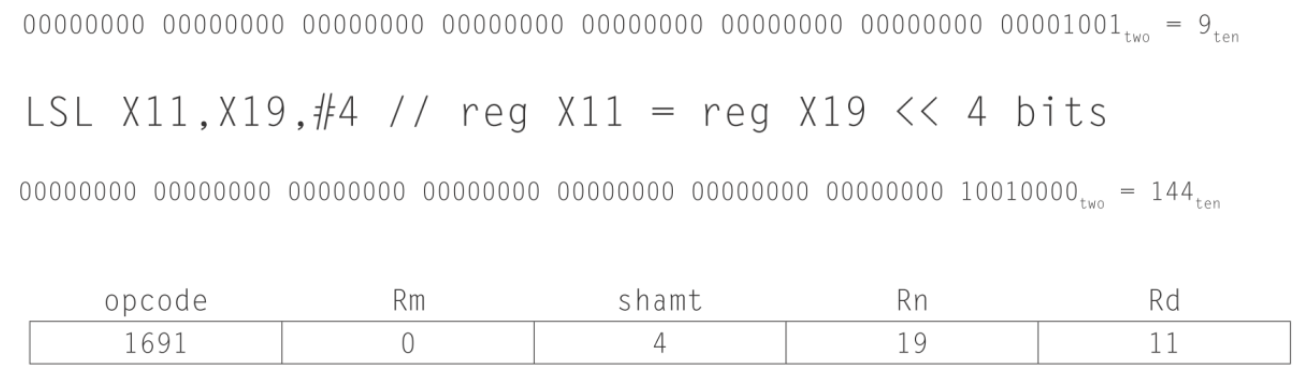
\includegraphics[width=0.7\columnwidth]{img/shift.png}
\end{center}
Un'altra operazione utile è l'\textbf{AND}. \'E un'operazione bit per bit che lascia un 1 nel risultato solo se entrambi i bit degli operandi sono 1.
\begin{center}
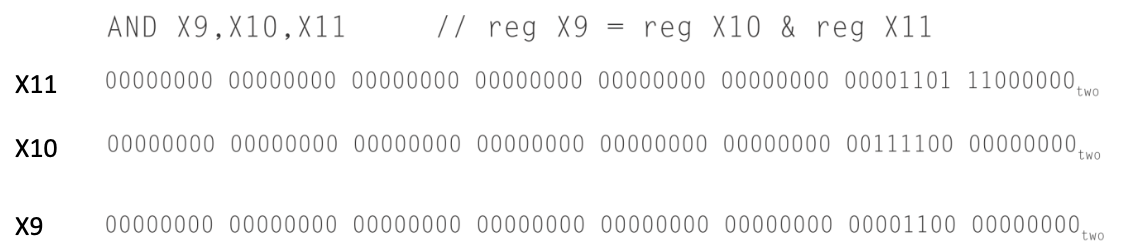
\includegraphics[width=0.7\columnwidth]{img/and.png}
\end{center}
\textbf{OR} è un'operazione bit-by-bit che pone un 1 nel risultato se uno dei bit operandi è un 1.
\begin{center}
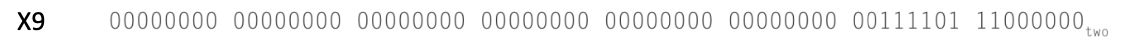
\includegraphics[width=0.7\columnwidth]{img/or.png}
\end{center}
\textbf{NOT} prende un operando e mette un 1 nel risultato se un bit di operando è uno 0 e viceversa. In linea con il formato a tre operandi, i progettisti di ARMv8 hanno deciso di includere le istruzioni \textbf{EOR} (OR esclusivo) invece di NOT. Poiché l'EOR crea uno 0 quando i bit sono gli stessi e un 1 se sono diversi
\begin{center}
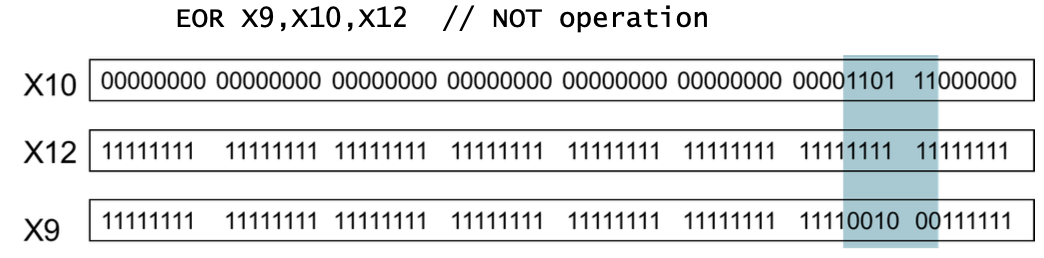
\includegraphics[width=0.7\columnwidth]{img/eor.png}
\end{center}
Le costanti sono utili nelle operazioni logiche e nelle operazioni aritmetiche, quindi LEGv8 fornisce anche le istruzioni AND immediate (ANDI), OR immediate (ORRI) ed EOR immediate (EORI).

\subsection{Differenze tra ARMv8 e LEGv8}
\begin{itemize}
\item I campi immediati per ANDI, ORRI ed EORI del set completo di istruzioni ARMv8 non sono semplici immediati a 12 bit. ARMv8 ha l'insolita caratteristica di utilizzare un algoritmo complesso per la codifica di valori immediati. Qualche piccola costante (e.g. 1, 2, 3, 4 e 6) sono valide, mentre altre (e.g. 0, 5) non lo sono. LEGv8 utilizza semplicemente normali immediate a 12 bit come si trova in ADDI. Questa differenza significa che EORI X1, X1, \#5 è legale per LEGv8 ma non ARMv8.
\item A differenza di quasi tutte le altre architetture informatiche, ARMv8 consente di spostare un registro come parte di un'istruzione aritmetica o logica. Poiché questa combinazione è insolita nelle architetture dei computer e non frequentemente generata dai compilatori, LEGv8 tratta gli shift come istruzioni separate. L'opcode utilizzato è quello di UBFM (unsignedbitfield move), ma la codifica dei campi Rm e shamt è stata semplificata.
\end{itemize}

\subsection{Istruzioni per prendere decisioni}
Il processo decisionale è comunemente rappresentato nei linguaggi di programmazione utilizzando l'istruzione if, a volte combinata con istruzioni ed etichette go to.\\
LEGv8 include due istruzioni decisionali, simili a una dichiarazione if con un go to.
\begin{center}
\begin{minipage}{.2\linewidth}
\begin{verbatim}
CBZ register, L1
\end{verbatim}
\end{minipage}
\end{center}
Significa andare all'istruzione etichettata L1 se il valore nel registro è uguale a zero.\\
\textbf{CBZ} sta per confrontare e ramificare se zero.
\begin{center}
\begin{minipage}{.2\linewidth}
\begin{verbatim}
CBNZ register, L1
\end{verbatim}
\end{minipage}
\end{center}
Significa andare all'istruzione etichettata L1 se il valore nel registro non è uguale a zero.\\
\textbf{CBNZ} sta per confronto e ramo se non zero.


\subsection{Compilazione degli $if-else$}
\begin{center}
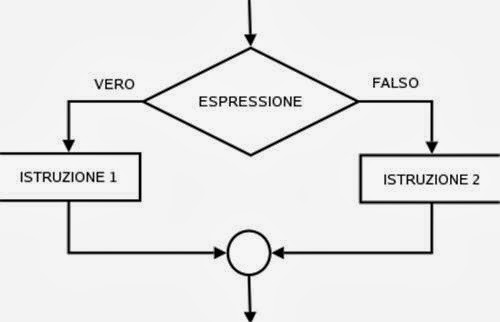
\includegraphics[width=0.7\columnwidth]{img/if.jpg}
\end{center}
f, g, h, i e j sono variabili che corrispondono ai cinque registri da X19 a X23.\\
Qual è il codice LEGv8 compilato per questa istruzione if in C?
\begin{center}
\begin{minipage}{.4\linewidth}
\begin{verbatim}
if (i == j)
       f = g + h;
else
       f = g - h;
\end{verbatim}
\end{minipage}
\end{center}
in LEGv8:
\begin{verbatim}
SUB X9, X22, X23 // X9 = i - j
CBNZ X9, Else // go to Else se i è diverso da j
ADD X19, X20, X21 // f = g + h
B Exit // go to Exit

Else: 
       SUB X19, X20, X21 // f = g - h

Exit:
\end{verbatim}

\subsection{Compilazione dei cicli $while$}
\begin{center}
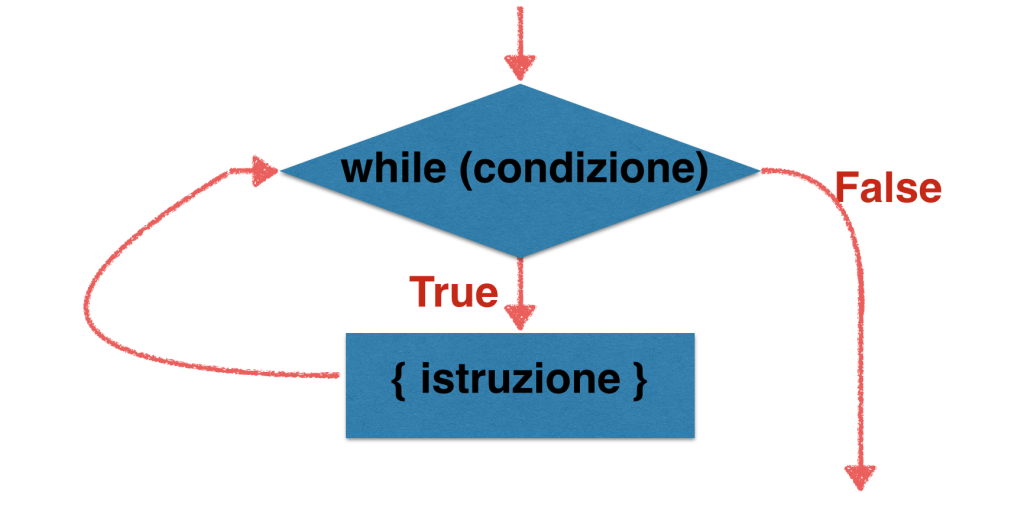
\includegraphics[width=0.7\columnwidth]{img/while.png}
\end{center}
Ecco un ciclo tradizionale in C:
\begin{center}
\begin{minipage}{.4\linewidth}
\begin{verbatim}
while (save[i] == k)
       i += 1;
\end{verbatim}
\end{minipage}
\end{center}
Supponiamo che i e k corrispondano ai registri X22 e X24 e la base del salvataggio dell'array sia in X25.\\
Qual è il codice di assemblaggio LEGv8 corrispondente a questo codice C?
\begin{verbatim}
Loop:
       LSL X10, X22, #3 // Temp reg X10 = i * 8
       ADD X10, X10, X25 // X10 = indirizzo di save[i]
       LDUR X9, [X10, #0] // Temp reg X9 = save[i]
       SUB X11, X9, X24 // X11 = save[i] - k
       CBNZ X11, Exit // go to Exit se save[i] è diverso da k
       ADDI X22, X22, #1 // i = i+1
       B Loop // go to Loop

Exit:
\end{verbatim}

\subsection{Blocchi base}
Un blocco di base è una sequenza di istruzioni con:
\begin{itemize}
\item Nessun salto (branch) (tranne eventualmente alla fine) 
\item Nessun branch target o branch label (tranne eventualmente all'inizio).
\end{itemize}
Un compilatore identifica i blocchi di base per l'ottimizzazione. Un processore avanzato può accelerare l'esecuzione di blocchi di base.

\subsection{Altre operazioni condizionali}
L'insieme dei confronti è: minore di (<), minore uguale di ($\leq$), maggiore di (>), maggiore uguale di ($\geq$), uguale (=) e diverso ($\not =$).\\
I confronti devono anche riguardare la dicotomia tra numeri con segno e senza segno. I codici di condizione o le flag vengono utilizzati per gestire tutti questi casi:\begin{itemize}
\item Negativo (N): il risultato settato dalla condizione ha un 1 nel bit più significativo
\item Zero (Z): il risultato settato dalla condiziona condizione è 0
\item Overflow (V): il risultato settato dalla condizione condizione è in overflow
\item Carry (C): Il risultato settato dalla condizione ha avuto un carry out del bit più significativo o un borrow nel bit più significativo
\end{itemize}
Sono impostati da un numero limitato di operazioni quando il codice delle condizioni è attivo: ADD, ADDI, AND, ANDI, SUB e SUBI.\\
Nel linguaggio assembly LEGv8, bisogna aggiungere una S alla fine di una di queste istruzioni se vuoi impostare una flag per un confronto: ADDS, ADDIS, ANDS, ANDIS, SUBS e SUBIS.\\
I salti condizionali (scritti come B.cond) usano combinazioni dei codici delle condizioni. Per salti condizionati da un confronto si utilizzano i seguenti codici:
\begin{itemize}
\item B.EQ (equal)
\item B.NE (not equal)
\item B.LT (less than, signed), B.LO (less than, unsigned)
\item B.LE (less than or equal, signed), B.LS (less than or same, unsigned)
\item B.GT (greater than, signed), B.HI (greater than, unsigned)
\item B.GE (greater than or equal, signed), B.HS (greater than or same, unsigned)
\end{itemize}
\begin{center}
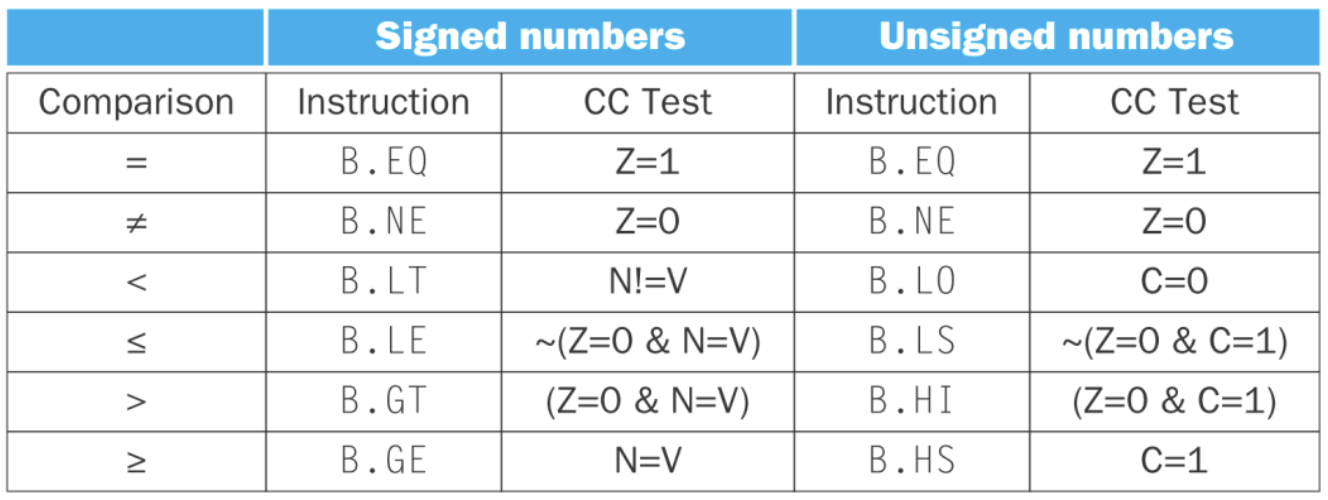
\includegraphics[width=0.7\columnwidth]{img/comparison.png}
\end{center}

\subsubsection{Esempio}
Codice C:
\begin{center}
\begin{minipage}{.4\linewidth}
\begin{verbatim}
if(a > b)
      a += 1;
\end{verbatim}
\end{minipage}
\end{center}
a in X22, b in X23\\
Il corrispondente codice Assembly LEGv8:
\begin{verbatim}
SUBS X9, X22, X23 // uso subtract per fare la comparazione
B.LE Exit
ADDI X22, X22, #1

Exit: ...
\end{verbatim}

\subsection{Supporto delle Procedure nei Computer}
\textbf{Procedura}: Una subroutine memorizzata che esegue un'attività specifica in base ai parametri con cui viene fornita. Le procedure sono un modo per implementare l'astrazione nel software.\\
Nell'esecuzione di una procedura, il programma deve seguire questi sei passaggi:
\begin{enumerate}
\item Metti i parametri in un luogo in cui la procedura possa accedervi.
\item Trasferisci il controllo alla procedura.
\item Acquisisci le risorse di archiviazione necessarie per la procedura.
\item Esegui il compito desiderato.
\item Metti il valore del risultato in un luogo in cui il programma chiamante può accedervi.
\item Restituire il controllo al punto di origine, poiché una procedura può essere chiamata da più punti in un programma.
\end{enumerate}

\subsubsection{Supporto del LEGv8 alle procedure}
Il software LEGv8 segue la seguente convenzione per la procedura che chiama l'assegnazione dei suoi 32 registri:
\begin{itemize}
\item X0 - X7: Otto registri di parametri in cui passare parametri o restituire valori.
\item LR (X30): un registro dell'indirizzo di ritorno per tornare al punto di origine.
\end{itemize}
Il linguaggio assembly LEGv8 include un'istruzione solo per le procedure: \textbf{branch-and-link (BL)} 
\begin{center}
\begin{minipage}{.4\linewidth}
\begin{verbatim}
BL ProcedureAddress
\end{verbatim}
\end{minipage}
\end{center}
Salta in un indirizzo e contemporaneamente salva l'indirizzo delle seguenti istruzioni, cioè l'indirizzo di ritorno nel registro LR (X30).\\
Per supportare il ritorno da una procedura, le architetture come LEGv8 usano l'istruzione del branch register (BR) che significa un salto incondizionato all'indirizzo specificato in un registro:
\begin{center}
\begin{minipage}{.4\linewidth}
\begin{verbatim}
BL LR
\end{verbatim}
\end{minipage}
\end{center}
Implicita nell'idea del programma memorizzato è la necessità di avere un registro per tenere l'indirizzo dell'istruzione corrente in esecuzione, il contatore del programma.

\subsubsection{Usando più registri}
Supponiamo che un compilatore abbia bisogno di più registri per una procedura rispetto agli otto registri degli argomenti. Tutti i registri necessari al chiamante devono essere ripristinati ai valori che contenevano prima dell'invocazione della procedura.\\
La struttura dati ideale per versare i registri è uno stack, una coda last-in-first-out. Uno stack ha bisogno di un puntatore, lo \textbf{stack pointer}, all'indirizzo allocato più di recentemente nello stack. Il puntatore dello stack (\textbf{SP}), che è solo uno dei 32 registri, viene regolato da una doubleword per ciascun registro che viene salvato o ripristinato.\\
\textbf{N.B.} SP è in X28 in LEGv8, ma in X31 in ARMv8.\\
Posizionare i dati sullo stack è chiamato \textbf{push} e la rimozione dei dati dallo stack è chiamata \textbf{pop}.\\
Storicamente lo stack "cresce" dagli indirizzi più alti a quelli più bassi. Questa convenzione significa che si immettono i valori sullo stack sottraendo dallo stack pointer. L'aggiunta allo stack pointer riduce lo stack, pulendo così i valori dello stack.

\subsubsection{Compilazione di una procedura che non chiama un'altra procedura}
\begin{verbatim}
long long int leaf_example (long long int g, long long int h, long long int i, 
long long int j)
{
      long long int f;
      
      f = (g + h) - (i + j);
      return f;
}
\end{verbatim}
Le variabili di parametro g, h, i e j corrispondono ai registri degli argomenti X0, X1, X2 e X3, f corrisponde a X19.\\
In Assembly:
\begin{verbatim}
leaf_example:
      SUBI SP, SP, #24 // crea lo spazio nello stack per 3 oggetti
      STUR X10, [SP,#16] // salva il registro X10 per utilizzarlo in seguito
      STUR X9,  [SP,#8] // salva il registro X9 per utilizzarlo in seguito
      STUR X19, [SP,#0] // salva il registro X19 per utilizzarlo in seguito
      
      ADD X9, X0, X1 // il registro X9 ora contiene g + h
      ADD X10, X2, X3 // il registro X10 ora contiene i + j
      SUB X19, X9, X10 // f = X9 - X10, che equivale a (g + h) - (i + j)
      
      ADD X0, X19, XZR // ritorna f (X0 = X19 + 0)
      
      LDUR X19, [SP,#0] // pulisce il registro X19 chiamato in precedenza
      LDUR X9, [SP,#8] // pulisce il registro X9 chiamato in precedenza
      LDUR X10, [SP,#16] // pulisce il registro X10 chiamato in precedenza
      ADDI SP, SP, #24 // ripristina lo stack
      
      BR LR // torna alla routine principale
\end{verbatim}
\begin{center}
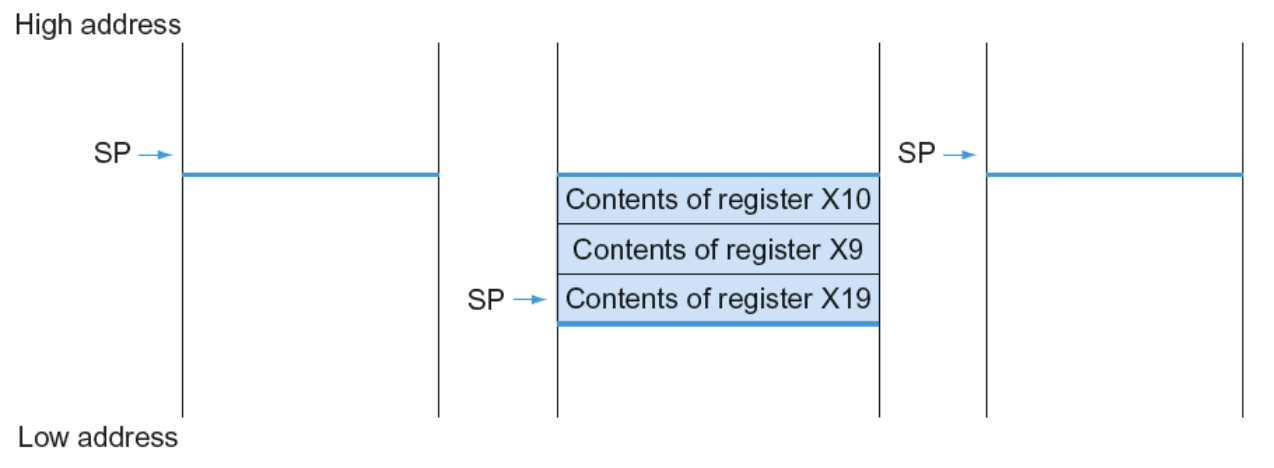
\includegraphics[width=0.7\columnwidth]{img/stack_ex.png}
\end{center}

\subsubsection{Utilizzo dei registri}
Abbiamo usato registri temporanei e abbiamo assunto che i loro vecchi valori dovessero essere salvati e ripristinati. Per evitare di salvare e ripristinare un registro il cui valore non viene mai utilizzato, il software LEGv8 separa 19 dei registri in due gruppi:
\begin{itemize}
\item X9 - X17: registri temporanei che non sono conservati dal chiamante su un chiamata alla procedura.
\item X19 - X28: registri salvati che devono essere conservati durante una chiamata alla procedura (se utilizzato, il chiamante salva e li ripristina).
\end{itemize}

\subsection{Procedure Non-Leaf}
Le procedure Non-Leaf sono procedure che chiamano altre procedure Per le chiamate nidificate, il chiamante deve salvare sullo stack:
\begin{itemize}
\item Il suo indirizzo di ritorno LR
\item Qualsiasi argomento (X0 - X7) e temporanei (X9 - X17) necessari dopo la chiamata
\end{itemize}
Ripristinare lo stack dopo la chiamata

\subsubsection{Esempio}
Codice C:
\begin{verbatim}
int fact (int n)
{
      if (n < 1)
            return f;
      else
            return n * fact(n-1);
}
\end{verbatim}
Argomento n in X0, risultato in X1 (\textcolor{red}{insolito, dovrebbe essere in X0})\\
Codice Assembly:
\begin{verbatim}
fact:
      SUBI SP, SP, #16 // crea lo spazio nello stack per 2 oggetti
      STUR  LR, [SP,#8] // salva l'indirizzo di ritorno
      STUR  X0, [SP,#0] // salva l'argomento n

      SUBIS XZR, X0, #1 // test for n < 1 
      B.GE L1 // if n >= 1, go to L1
      
      ADDI X1, XZR, #1 // ritorna 1
      ADDI SP, SP, #16 // poppa 2 oggetti dallo stack
      BR LR // salta al chiamante
      
L1:
      SUBI X0, X0, #1 // n >= : l'argomento diventa (n - 1)
      BL fact // chiama fact con (n - 1)
      
      LDUR X0, [SP, #0] // reimposta l'argomento n
      LDUR LR, [SP, #8] // ripulisce il registro di ritorno
      ADDI SP, SP, #16 // ripristina lo stack
      MUL X1, X0, X1 // ritorna n * fact(n - 1)
      BR LR // salta al chiamante
\end{verbatim}

\subsubsection{Conservato / Non conservato tra le chiamate}
\begin{center}
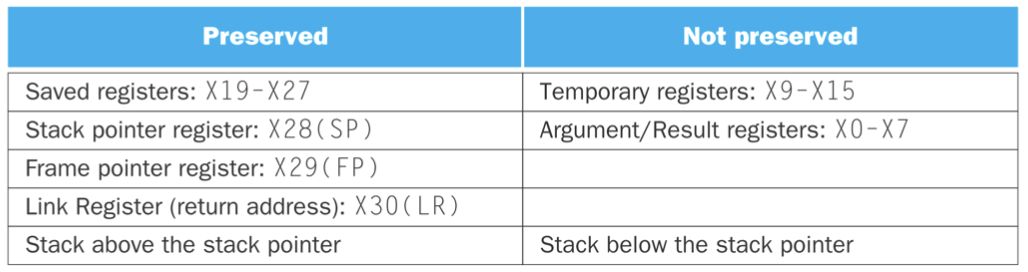
\includegraphics[width=0.7\columnwidth]{img/preserved.png}
\end{center}

\subsection{Gestione delle variabili C}
Una variabile C è generalmente una posizione nello storage e la sua interpretazione dipende sia dal suo tipo che dalla sua classe di archiviazione. I tipi di esempio includono numeri interi e caratteri. Il linguaggio C ha due classi di archiviazione: automatica e statica. Le variabili automatiche sono locali a una procedura e vengono eliminate quando la procedura esce. Esistono invece variabili statiche tra le uscite e le chiamate alle procedure. Vengono dichiarate al di fuori di tutte le procedure o utilizzando la parola chiave static.\\
Per semplificare l'accesso ai dati statici, alcuni compilatori LEGv8 riservano un registro, chiamato \textbf{global pointer}, o GP, ad esempio X27.\\
Le variabili automatiche vengono salvate nei registri o nello stack.\\
Le variabili statiche vengono salvate nel segmento dei dati statici.\\
La memoria allocata dinamicamente viene posizionata nell'heap.\\

\subsection{Struttura delle procedure}
Il segmento dello stack che contiene il registro di salvataggio di una procedura e delle variabili locali viene chiamato \textbf{procedure frame} o \textbf{activation record}.\\
Alcuni compilatori ARMv8 usano un \textbf{frame pointer} (FP) per puntare alla prima doubleword del frame di una procedura. Un puntatore dello stack potrebbe cambiare durante la procedura. Un frame pointer offre un registro di base stabile all'interno di una procedura per i riferimenti alla memoria locale.
\begin{center}
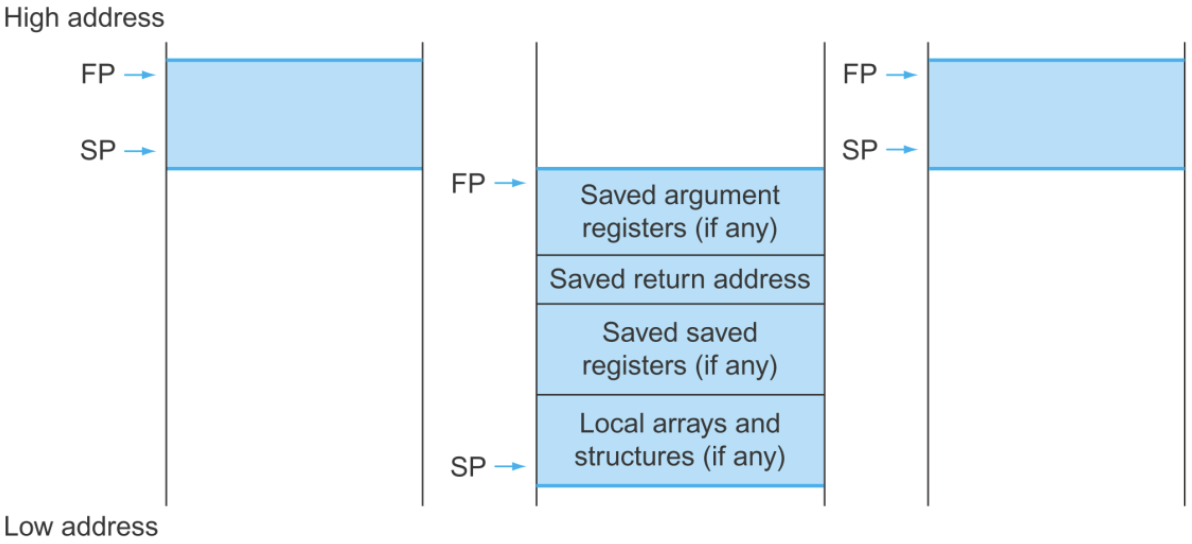
\includegraphics[width=0.7\columnwidth]{img/procedure_frame.png}
\end{center}

\subsection{Layout della Memoria}
\begin{center}
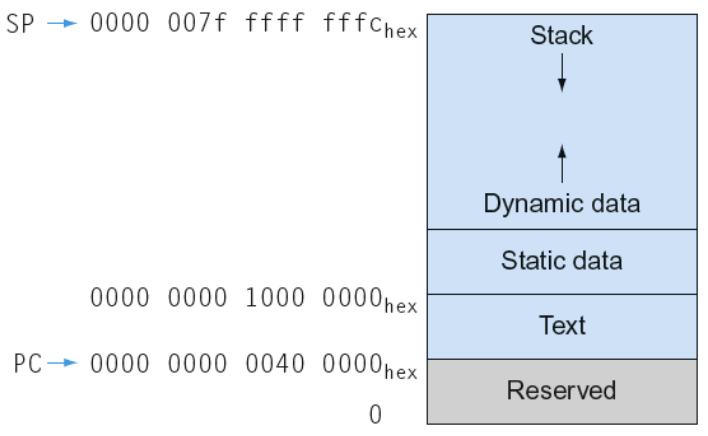
\includegraphics[width=0.7\columnwidth]{img/memory_layout.png}
\end{center}
\begin{itemize}
\item \textbf{Text}: Codice del programma
\item \textbf{Static data}: Variabili globali (e.g. variabili statiche in C, array costanti e stringhe)
\item \textbf{Dynamic data}: Heap (e.g. malloc in C, new in Java)
\item \textbf{Stack}: Storage automatico
\end{itemize}

\subsection{Sommario delle convenzioni dei registri}
\begin{center}
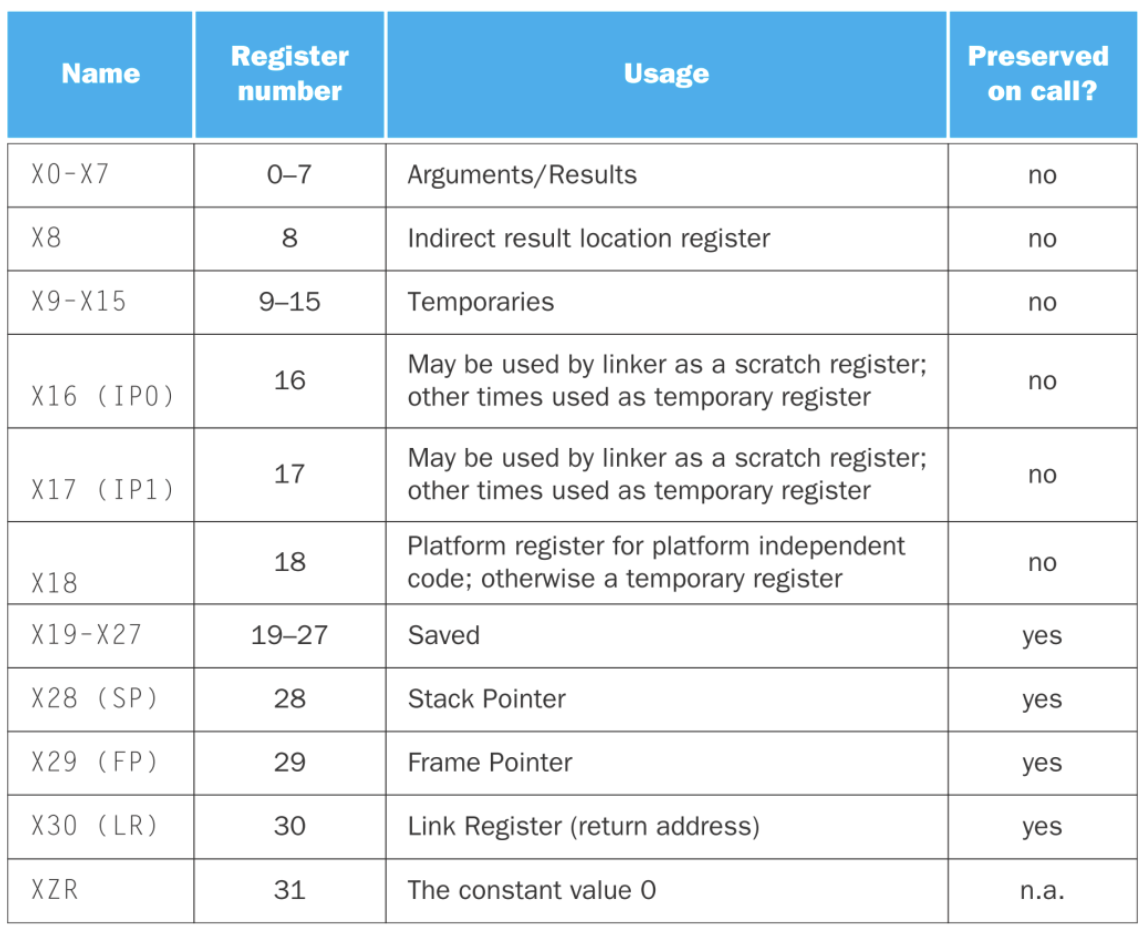
\includegraphics[width=0.7\columnwidth]{img/summary_register.png}
\end{center}

\subsection{Operazioni Byte/Halfword}
LEGv8 byte/halfword Load/Store
\begin{itemize}
\item Load byte: 
\begin{minipage}{.2\linewidth}
\begin{verbatim}
LDURB Rt, [Rn, offset]
\end{verbatim}
\end{minipage}
\item Store byte:
\begin{minipage}{.2\linewidth}
\begin{verbatim}
STURB Rt, [Rn, offset]
\end{verbatim}
\end{minipage}
\item Load halfword:
\begin{minipage}{.2\linewidth}
\begin{verbatim}
LDURH Rt, [Rn, offset]
\end{verbatim}
\end{minipage}
\item Store halfword:
\begin{minipage}{.2\linewidth}
\begin{verbatim}
STURH Rt, [Rn, offset]
\end{verbatim}
\end{minipage}
\end{itemize}
LEGv8 word load/store
\begin{itemize}
\item Load signed word:
\begin{minipage}{.2\linewidth}
\begin{verbatim}
LDURSW Rt, [Rn, offset]
\end{verbatim}
\end{minipage}
\item Store word:
\begin{minipage}{.2\linewidth}
\begin{verbatim}
STURW Rt, [Rn, offset]
\end{verbatim}
\end{minipage}
\end{itemize}

\subsection{Esempio "String Copy"}
Codice C:
\begin{verbatim}
void strcpy (char x[ ], char y[ ])
{
      size_t i;
      i = 0;
      
      while ( x[i] = y[i] != '\0')
            i += 1;
}
\end{verbatim}
Gli indirizzi di base per gli array x e y si trovano in X0 e X1, mentre i si trova in X19.\\
Codice LEGv8:
\begin{verbatim}
strcpy:
      SUBI SP, SP, 8 // push X19
      STUR X19, [SP, #0]
      ADD X19, XZR, XZR // i = 0

L1:
      ADD X10, X19, X1 // X10 = indirizzo di y[i]
      LDURB X11, [X10,#0] // X11 = y[i]
      ADD X12, X19, X0 // X12 = indirizzo di x[i]
      STURB X11, [X12,#0] // y[i] = x[i]
      CBZ X11, L2 // if y[i] == 0 esci
      ADDI X19, X19, #1 // i = i + 1
      B L1 //prossima iterazione

L2:
      LDUR X19, [SP, #0] // restore delle variabili
      ADDI SP, SP, 8 // pop di 1 elemento dallo stack
      BR LR // ritorna alla funzione chiamante
\end{verbatim}
\textbf{Nota Bene}: I software per ARMv8 richiedono che lo stack si allinei gli indirizzi delle quadword (16 byte) per avere delle performance migliori. Questa convenzione significa che una variabile char allocata sullo stack occupa 16 byte, anche se ne ha bisogno di meno. Tuttavia, una variabile stringa C o una matrice di byte imballerà 16 byte per quadword.\\
LEGv8 mantiene tutto a 64 bit rispetto a fornire istruzioni di indirizzo sia a 32 bit che a 64 bit come in ARMv8, il che significa che deve includere STURW (memorizzazione di parole) come istruzione anche se non è specificato in ARMv8 nel linguaggio assembly. ARMv8 utilizza solo STUR con un nome di registro W (registro a 32 bit) invece del nome del registro X (registro a 64 bit).

\subsection{Operandi Immediati ampi}
La maggior parte delle costanti sono piccole e l'immediato a 12 bit è sufficiente.\\
Per la costante occasionale a 32 bit
\begin{itemize}
\item \textbf{MOVZ}: muoviti ampio con zeri
\item \textbf{MOVK}: muoviti ampio con keep
\end{itemize}
Può impostare qualsiasi 16 bit di una costante in un registro. Il campo a 16 bit da caricare viene specificato aggiungendo LSL e quindi il numero 0, 16, 32 o 48.
\begin{center}
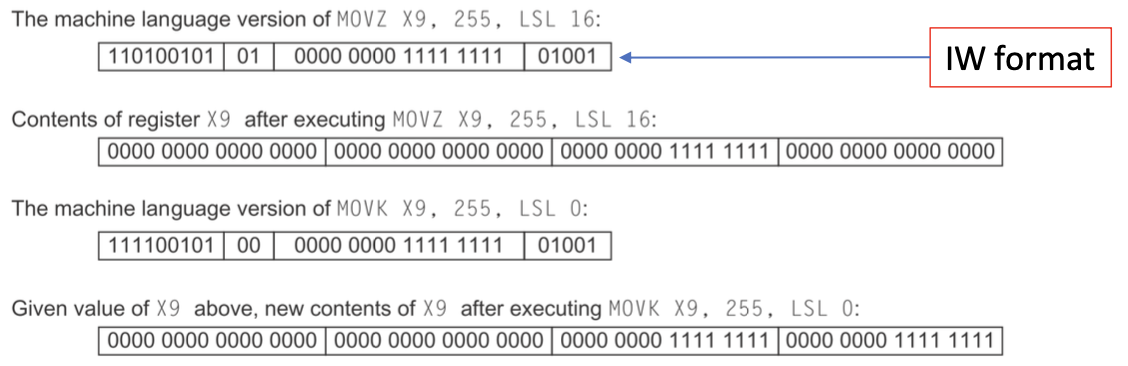
\includegraphics[width=0.7\columnwidth]{img/mov.png}
\end{center}

\subsection{Indirizzi nei salti}
Tipo B: \begin{minipage}{.2\linewidth}
\begin{verbatim}
B 1000 // go to location 100000 (base 10)
\end{verbatim}
\end{minipage}
\begin{center}\begin{tabular}{cc}
\hline
\multicolumn{1}{|c|}{5} & \multicolumn{1}{c|}{$100000_{ten}$}\\ \hline
6 bits & 26 bits                 
\end{tabular}\end{center}
Tipo CB: \begin{minipage}{.2\linewidth}
\begin{verbatim}
CBNZ X19, Exit // go to Exit if X19 != 0
\end{verbatim}
\end{minipage}
\begin{center}\begin{tabular}{ccc}
\hline
\multicolumn{1}{|c|}{181} & \multicolumn{1}{c|}{Exit} & \multicolumn{1}{c|}{19} \\ \hline
8 bits & 19 bits & 5 bits                   
\end{tabular}\end{center}
Entrambi gli indirizzi sono PC-relative. Indirizzo = PC + offset (dalle istruzioni)\\
Questa forma di indirizzamento dei branch si chiama PC-relative adressing.\\
Poiché tutte le istruzioni LEGv8 sono lunghe 4 byte, LEGv8 allunga la distanza del ramo avendo PC-relative addressing si riferisce al numero di parole all'istruzione successiva invece che al numero di byte.
\begin{itemize}
\item Il campo a 19 bit può diramarsi di $\pm$ 1 MB dal PC corrente
\item Il campo a 26 bit può diramarsi $\pm$ 128 MB dal PC corrente
\end{itemize}
La maggior parte dei salti condizionali si trova in una posizione vicina, ma occasionalmente si salta più lontano, più lontano di quanto possa essere rappresentato nei 19 bit dell'istruzione del salto condizionale. In questi casi l'assembler viene in soccorso!\\
Dato \begin{center}\begin{minipage}{.2\linewidth}
\begin{verbatim}
CBZ X19, L1
\end{verbatim}
\end{minipage}\end{center}
Può sostituire il salto condizionale a indirizzi brevi con
\begin{verbatim}
      CBNZ X19, L2
      B L1
L2:
\end{verbatim}

\subsection{Sintesi della modalità di indirizzamento LEGv8}
Le modalità di indirizzamento delle istruzioni LEGv8 sono le seguenti:
\begin{enumerate}
\item Indirizzamento immediato, dove l'operando è una costante all'interno dell'istruzione stessa.
\begin{center}
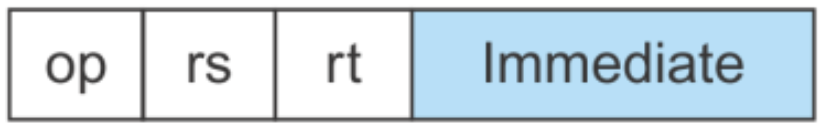
\includegraphics[width=0.4\columnwidth]{img/immediate_adressing.png}
\end{center}
\item Indirizzamento del registro, dove l'operando è un registro.
\begin{center}
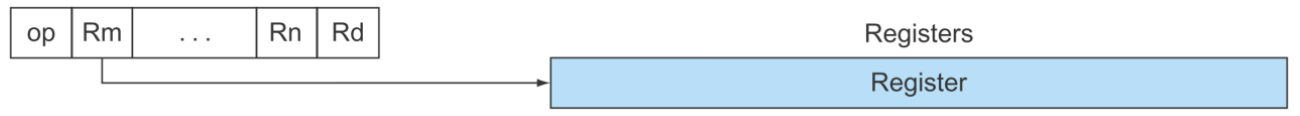
\includegraphics[width=0.6\columnwidth]{img/register_adressing.png}
\end{center}
\item Indirizzamento di base o spostamento, dove l'operando si trova nella posizione di memoria il cui indirizzo è la somma di un registro e di una costante nell'istruzione, ad es. LDUR, STUR
\begin{center}
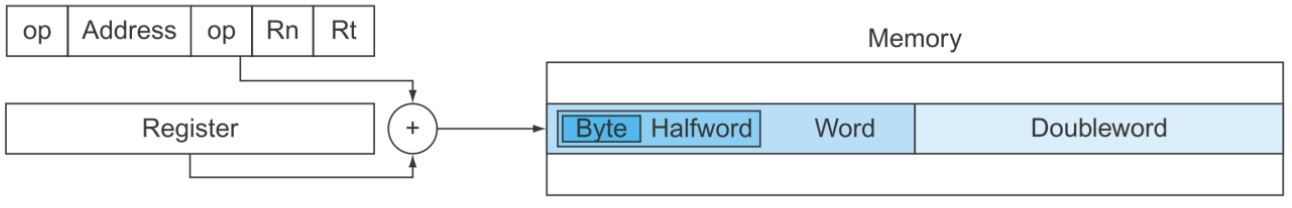
\includegraphics[width=0.6\columnwidth]{img/base_adressing.png}
\end{center}
\item Indirizzamento relativo al PC, dove l'indirizzo della filiale è la somma del PC e una costante nel istruzione.
\begin{center}
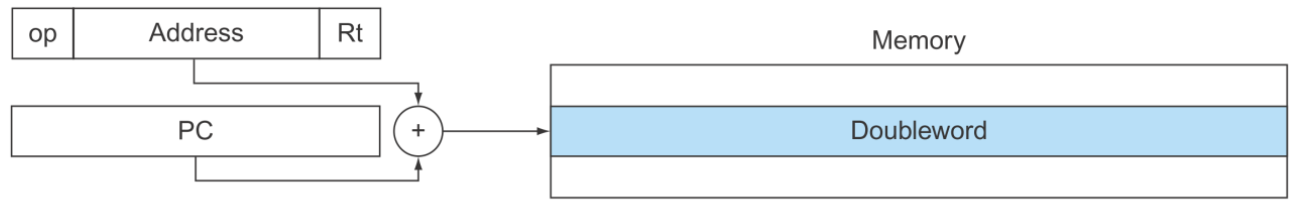
\includegraphics[width=0.6\columnwidth]{img/pc_adressing.png}
\end{center}
\end{enumerate}

\subsection{Sintesi della codifica LEGv8}
\Sep
\begin{center}
\begin{tabular}{|l|ccccccc|}
\hline
\rowcolor[HTML]{FFC702} 
\multicolumn{1}{|c|}{\cellcolor[HTML]{FFC702}Nome} & \multicolumn{7}{c|}{\cellcolor[HTML]{FFC702}Campi}                                                                                                                                                     \\ \hline
Grandezza campi                                    & \multicolumn{1}{c|}{}   & \multicolumn{1}{c|}{6 to 11 bits} & \multicolumn{1}{c|}{5 to 10 bits} & \multicolumn{1}{c|}{5 o 4 bits} & \multicolumn{1}{c|}{2 bits} & \multicolumn{1}{c|}{5 bits} & 5 bits \\ \hline
Formato R                                          & \multicolumn{1}{c|}{R}  & \multicolumn{1}{c|}{opcode}       & \multicolumn{1}{c|}{Rm}           & \multicolumn{2}{c|}{shamt}                                    & \multicolumn{1}{c|}{Rn}     & Rd     \\ \hline
Formato I                                          & \multicolumn{1}{c|}{I}  & \multicolumn{1}{c|}{opcode}       & \multicolumn{3}{c|}{immediate}                                                                    & \multicolumn{1}{c|}{Rn}     & Rd     \\ \hline
Formato D                                          & \multicolumn{1}{c|}{D}  & \multicolumn{1}{c|}{opcode}       & \multicolumn{2}{c|}{address}                                        & \multicolumn{1}{c|}{op2}    & \multicolumn{1}{c|}{Rn}     & Rt     \\ \hline
Formato B                                          & \multicolumn{1}{c|}{B}  & \multicolumn{1}{c|}{opcode}       & \multicolumn{5}{c|}{address}                                                                                                             \\ \hline
Formato CB                                         & \multicolumn{1}{c|}{CB} & \multicolumn{1}{c|}{opcode}       & \multicolumn{4}{c|}{address}                                                                                                    & Rt     \\ \hline
Formato IW                                         & \multicolumn{1}{c|}{IW} & \multicolumn{1}{c|}{opcode}       & \multicolumn{4}{c|}{immediate}                                                                                                  & Rd     \\ \hline
\end{tabular}
\end{center}

\subsection{Parallelismo e Istruzioni: Sincronizzazione}
Due processori che condividono un'area di memoria\begin{itemize}
\item P1 scrive, poi P2 legge
\item Data race se P1 e P2 non si sincronizzano. Il risultato dipende dall'ordine di accesso
\end{itemize}
È richiesto il supporto hardware
\begin{itemize}
\item Funzionamento atomico della memoria di lettura/scrittura
\item Nessun altro accesso alla posizione consentito tra la lettura e la scrittura
\end{itemize}
Potrebbe essere una singola istruzione. Ad esempio, scambio atomico o una coppia atomica di istruzioni.\\
Supponiamo di voler costruire un semplice blocco in cui il valore 0 viene utilizzato per indicare che il lucchetto è libero e 1 viene utilizzato per indicare che il lucchetto non è disponibile. Un processore tenta di impostare il blocco facendo uno scambio di 1, che si trova in un registro, con l'indirizzo di memoria corrispondente al blocco. Il valore restituito dall'istruzione di scambio è 1 se qualche altro processore aveva già rivendicato l'accesso e 0 altrimenti. In quest'ultimo caso, anche il valore viene modificato in 1, impedendo a qualsiasi scambio concorrente in un altro processore di recuperare anche uno 0.

\subsubsection{Sincronizzazione in LEGv8}
LEGv8 include un load speciale e un store speciale chiamato:
\begin{itemize}
\item Registro esclusivo del carico (LDXR)
\item Registro esclusivo di store (STXR)
\end{itemize}
Queste istruzioni vengono utilizzate in sequenza.\\
Se il contenuto della posizione di memoria specificata da LDXR viene modificato prima dello STXR si verifica allo stesso indirizzo, quindi l'STXR fallisce e non scrive il valore in memoria.\\
L'STXR è definito sia per memorizzare il valore di un registro in memoria che per modificare il valore di un altro registro a uno 0 se ha successo e a un 1 se fallisce. STXR specifica tre registri: uno per tenere l'indirizzo, uno per indicare il fallimento o il successo e uno per tenere il valore da memorizzare in memoria.

\paragraph{Esempio 1: Atomic swap (to test/set lock variable)}
\begin{verbatim}
again:
       LDXR X10, [X20,#0] // Load esclusivo
       STXR X23, X9, [X20] // Store esclusivo
       CBNZ X9, again // Salta se store fallisce
       ADD X23, XZR, X10 // metti il valore caricato in x23
\end{verbatim}

\paragraph{Esempio 2: Lock}
\begin{verbatim}
       ADDI X11, XZR, #1 // Copia il valore
again:
       LDXR X10, [X20,#0] // Load esclusivo per leggere lock
       CBNZ X10, again // Controlla se è già a 0
       STXR X11, X9, [X20] // Prova a salvare il nuovo valore
       BNEZ X9, again // Salta se store fallisce
       ADD X23, XZR, X10 // metti il valore caricato in x23
unlock:
      STUR XZR, [X20,#0] // Libera lock scrivendoci 0
\end{verbatim}

\subsection{Tradurre e avviare un programma}
Per identificare il tipo di file, UNIX segue una convenzione di suffissi per i file:
\begin{itemize}
\item I file sorgente C si chiamano nome\_file.c
\item I file assembly sono nome\_file.s
\item I file oggetto si chiamano nome\_file.o
\item Le routine di libreria collegate staticamente sono nome\_file.a
\item Le routine della libreria collegate dinamicamente sono nome\_file.so
\item I file eseguibili sono chiamati nome\_file.out
\end{itemize}
\textbf{N.B.}: MS-DOS utilizza i suffissi .c, .asm, .obj, .lib, .dll e .exe con lo stesso effetto.
\begin{center}
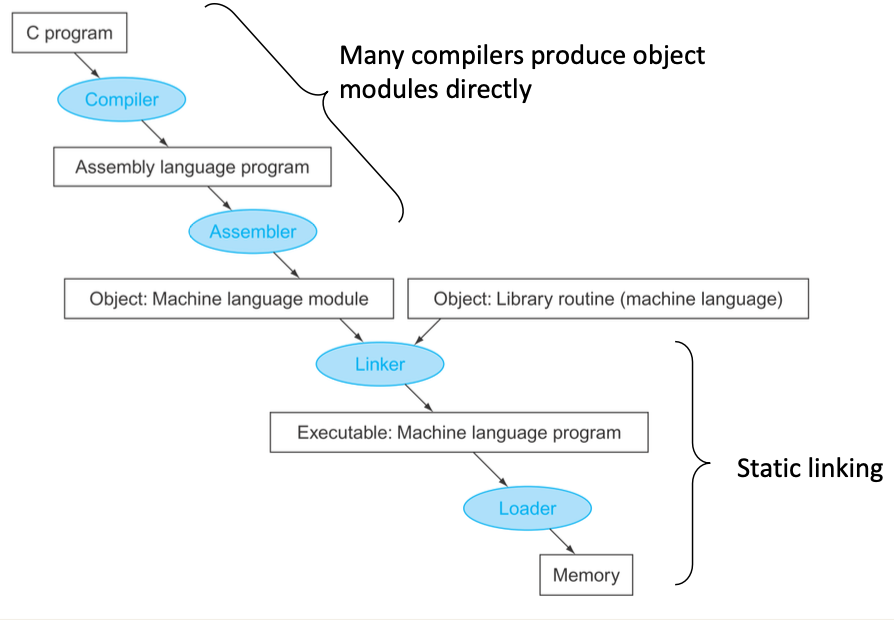
\includegraphics[width=0.7\columnwidth]{img/execution.png}
\end{center}

\subsubsection{Compilatore}
Il compilatore trasforma il programma C in un programma di linguaggio assembly. Nel 1975, molti sistemi operativi e assemblatori sono stati scritti in linguaggio assembly perché le memorie erano piccole e i compilatori erano inefficienti.\\
Oggi i compilatori possono produrre programmi di linguaggio assembly quasi quanto prodotto da un programmatore esperto di linguaggio assembly, e talvolta anche migliore per programmi di grandi dimensioni.

\subsubsection{Assemblatore}
L'assemblatore traduce il programma del linguaggio assembly in linguaggio macchina.\\
Crea un file oggetto, che è una combinazione di istruzioni sul linguaggio macchina, dati e informazioni necessarie per inserire correttamente le istruzioni in memoria.
L'assemblatore può anche trattare le variazioni comuni delle istruzioni del linguaggio della macchina, ad es. pseudoistruzioni. Ad esempio, LEGv8 accetta
\begin{verbatim}
MOV X9, X10 // Il registro X9 da il registro X10
\end{verbatim}
\begin{itemize}
\item Convertito a: \begin{minipage}{.2\linewidth}
\begin{verbatim}
ORR X9, XZR, X10 // Il registro X9 da 0 o il registro X10
\end{verbatim}
\end{minipage}
\end{itemize}
\begin{verbatim}
CMP X9, X10 // Compara X9 a X10 e setta le condizioni
\end{verbatim}
\begin{itemize}
\item Convertito a: \begin{minipage}{.2\linewidth}
\begin{verbatim}
SUBS XZR, X9, X10 // usa X9 - X10 per settare le condizioni
\end{verbatim}
\end{minipage}
\end{itemize}
\begin{verbatim}
AND X9, X10, #15 // Il registro X9 da X10 e #15
\end{verbatim}
\begin{itemize}
\item Convertito a: \begin{minipage}{.2\linewidth}
\begin{verbatim}
ANDI X9, X10, #15 // Il registro X9 da X10 e #15
\end{verbatim}
\end{minipage}
\end{itemize}
Per produrre la versione binaria di ogni istruzione nel programma del linguaggio assembly, l'assemblatore deve determinare gli indirizzi corrispondenti a tutte le etichette.\\
Gli assemblatori tengono traccia delle etichette utilizzate nei rami e delle istruzioni per il trasferimento dei dati in una tabella dei simboli. La tabella contiene coppie di simboli e indirizzi.\\
Il file oggetto per i sistemi UNIX contiene in genere sei pezzi distinti:
\begin{itemize}
\item L'intestazione del file oggetto (object file header) descrive le dimensioni e la posizione degli altri pezzi del file oggetto.
\item Il segmento di testo (text segment) contiene il codice del linguaggio macchina.
\item Il segmento di dati statici (static data segment) contiene dati allocati per tutta la vita del programma.
\item Le informazioni di trasferimento (relocation information) identificano istruzioni e parole di dati che dipendono dagli indirizzi assoluti quando il programma viene caricato in memoria.
\item La tabella dei simboli (symbolic table) contiene le etichette rimanenti che non sono definite, come quelle esterne riferimenti.
\item Le informazioni di debug (debugging information) contengono una descrizione concisa di come sono stati compilati i moduli in modo che un debugger possa associare le istruzioni della macchina ai file sorgente C
\end{itemize}

\subsubsection{Linker (anche chiamato linker editor)}
Il linker è un programma di sistema che combina programmi di linguaggio macchina assemblati in modo indipendente e risolve tutte le etichette non definite in un file eseguibile.\\
Ci sono tre passaggi per il linker:
\begin{enumerate}
\item Posiziona simbolicamente codice e moduli di dati in memoria.
\item Determina gli indirizzi dei dati e le etichette delle istruzioni.
\item Patcha sia i riferimenti interni che esterni.
\end{enumerate}
Il linker utilizza le informazioni di trasferimento e la tabella dei simboli in ciascun modulo oggetto per risolvere tutte le etichette non definite (cioè nelle istruzioni dei salti e negli indirizzi dei dati). Se tutti i riferimenti esterni vengono risolti, il linker determina successivamente le posizioni di memoria che ogni modulo occuperà. Quando il linker inserisce un modulo in memoria, tutti i riferimenti assoluti, cioè gli indirizzi di memoria che non sono relativi a un registro, devono essere spostati per riflettere la sua vera posizione.\\
Il linker produce un file eseguibile che può essere eseguito su un computer. Il file eseguibile è un programma funzionale nel formato di un file oggetto che non contiene riferimenti irrisolti, può contenere tabelle di simboli e informazioni sul debug. Le informazioni sul trasferimento possono essere incluse per il caricatore.

\paragraph{Esempio}
\Sep
\begin{center}
\begin{tabular}{|c|c|c|c|}
\hline
\textbf{Header del file oggetto} &                          &                                                &                          \\ \hline
                                 & Nome                     & Procedura A                                    &                          \\ \hline
                                 & Text Size                & $100_{hex}$                                    &                          \\ \hline
                                 & Data Size                & $20_{hex}$                                     &                          \\ \hline
Text Segment                     & Indirizzo                & Istruzione                                     &                          \\ \hline
                                 & 0                        &  LDUR X0, {[}X27, {\color[HTML]{3531FF}\#0{}}] &                          \\ \hline
                                 & 4                        & BL {\color[HTML]{3531FF} 0}                    &                          \\ \hline
                                 & \dots     & \dots                           &                          \\ \hline
Data Segment                     & {\color[HTML]{3531FF} 0} & ({\color[HTML]{3531FF} X})                     &                          \\ \hline
                                 & \dots     & \dots                           &                          \\ \hline
Informazioni di trasferimento    & Indirizzo                & Tipo di istruzione                             & Dipendenza               \\ \hline
                                 & 0                        & LDUR                                           & {\color[HTML]{3531FF} X} \\ \hline
                                 & 4                        & BL                                             & {\color[HTML]{3531FF} B} \\ \hline
Tabella simboli                  & Simbolo                  & Indirizzo                                      &                          \\ \hline
                                 & {\color[HTML]{3531FF} X} & -                                              &                          \\ \hline
                                 & {\color[HTML]{3531FF} B} & -                                              &                          \\ \hline
\end{tabular}
\end{center}

\begin{center}
\begin{tabular}{|c|c|c|c|}
\hline
                                 & Nome                     & Procedura B                                  &                          \\ \hline
                                 & Text Size                & $200_{hex}$                                    &                          \\ \hline
                                 & Data Size                & $30_{hex}$                                     &                          \\ \hline
Text Segment                     & Indirizzo                & Istruzione                                     &                          \\ \hline
                                 & 0                        &  STUR X1, {[}X27, {\color[HTML]{3531FF}\#0{}}] &                          \\ \hline
                                 & 4                        & BL {\color[HTML]{3531FF} 0}                    &                          \\ \hline
                                 & \dots     & \dots                           &                          \\ \hline
Data Segment                     & {\color[HTML]{3531FF} 0} & ({\color[HTML]{3531FF} Y})                     &                          \\ \hline
                                 & \dots     & \dots                           &                          \\ \hline
Informazioni di trasferimento    & Indirizzo                & Tipo di istruzione                             & Dipendenza               \\ \hline
                                 & 0                        & STUR                                           & {\color[HTML]{3531FF} Y} \\ \hline
                                 & 4                        & BL                                             & {\color[HTML]{3531FF} A} \\ \hline
Tabella simboli                  & Simbolo                  & Indirizzo                                      &                          \\ \hline
                                 & {\color[HTML]{3531FF} Y} & -                                              &                          \\ \hline
                                 & {\color[HTML]{3531FF} A} & -                                              &                          \\ \hline
\end{tabular}
\end{center}

\begin{center}
\begin{tabular}{|c|c|c|}
\hline
\textbf{File header eseguibile} &                                &                                                         \\ \hline
                                & Text Size                      & $300_{hex}$                                             \\ \hline
                                & Data Size                      & $50_{hex}$                                              \\ \hline
Text Segment                    & Indirizzo                      & Istruzione                                              \\ \hline
                                & $0000\ 0000\ 0040\ 0000_{hex}$ & LDUR X0, {[}X27,  {\color[HTML]{3531FF}\#$0_{hex}${}}]  \\ \hline
                                & $0000\ 0000\ 0040\ 0004_{hex}$ & BL {\color[HTML]{3531FF} $000\ 00FC_{hex}$}             \\ \hline
                                & \dots                           & \dots                                                    \\ \hline
                                & $0000\ 0000\ 0040\ 0100_{hex}$ & STUR X1, {[}X27, {\color[HTML]{3531FF} \#$20_{hex}${}}] \\ \hline
                                & $0000\ 0000\ 0040\ 0104_{hex}$ & BL {\color[HTML]{3531FF} $3FF\ FEFC_{hex}$}             \\ \hline
                                & \dots                           & \dots                                                    \\ \hline
Data Segment                    & Indirizzo                      & {\color[HTML]{FFCB2F} }                                 \\ \hline
                                & $0000\ 0000\ 1000\ 0000_{hex}$ & ({\color[HTML]{3531FF} X})                              \\ \hline
                                & \dots                           & \dots                                                    \\ \hline
                                & $0000\ 0000\ 1000\ 0020_{hex}$ & ({\color[HTML]{3531FF} Y})                              \\ \hline
                                & \dots                           & \dots                                                    \\ \hline
\end{tabular}
\end{center}

\subsubsection{Loader}
Il loader è un programma di sistema che posiziona un programma oggetto nella memoria principale in modo che sia pronto per l'esecuzione.\\
Il loader segue questi passaggi nei sistemi UNIX:
\begin{enumerate}
\item Legge l'intestazione del file eseguibile per determinare le dimensioni dei segmenti di testo e dati.
\item Crea uno spazio di indirizzi abbastanza grande per il testo e i dati.
\item Copia le istruzioni e i dati dal file eseguibile in memoria.
\item Copia i parametri (se presenti) al programma principale sullo stack.
\item Inizializza i registri del processore e imposta il puntatore dello stack nella prima posizione libera.
\item Salta a una routine di avvio che copia i parametri nei registri degli argomenti e nelle chiama la routine principale del programma. Quando la routine principale ritorna, la routine di avvio termina il programma con una chiamata di uscita.
\end{enumerate}


\subsubsection{Librerie collegate dinamicamente (DLL)}
Abbiamo descritto il tradizionale approccio statico al collegamento delle librerie prima che il programma venga eseguito.\\
Ha alcuni svantaggi:
\begin{itemize}
\item Le routine della libreria diventano parte del codice eseguibile. Se viene rilasciata una nuova versione della libreria che corregge bug o supporta nuovi dispositivi hardware, il programma collegato staticamente continua a utilizzare la vecchia versione.
\item Carica tutte le routine nella libreria che vengono chiamate in qualsiasi punto dell'eseguibile, anche se tali chiamate non vengono eseguite. La libreria può essere grande rispetto al programma.
\end{itemize}
Questi svantaggi portano a librerie collegate dinamicamente (DLLs), in cui le routine di libreria non sono collegate e caricate fino all'esecuzione del programma. Sia il programma che le routine della libreria conservano informazioni aggiuntive sulla posizione delle procedure non locali e sui loro nomi.\\
Nella versione originale delle DLL, il loader esegue un linker dinamico, utilizzando le informazioni aggiuntive nel file per trovare le librerie appropriate e aggiornare tutti i riferimenti esterni. Ma collega ancora tutte le routine della librerie che potrebbero essere chiamate. In un approccio più efficiente ogni routine è collegata solo dopo essere stata chiamata.
\begin{center}
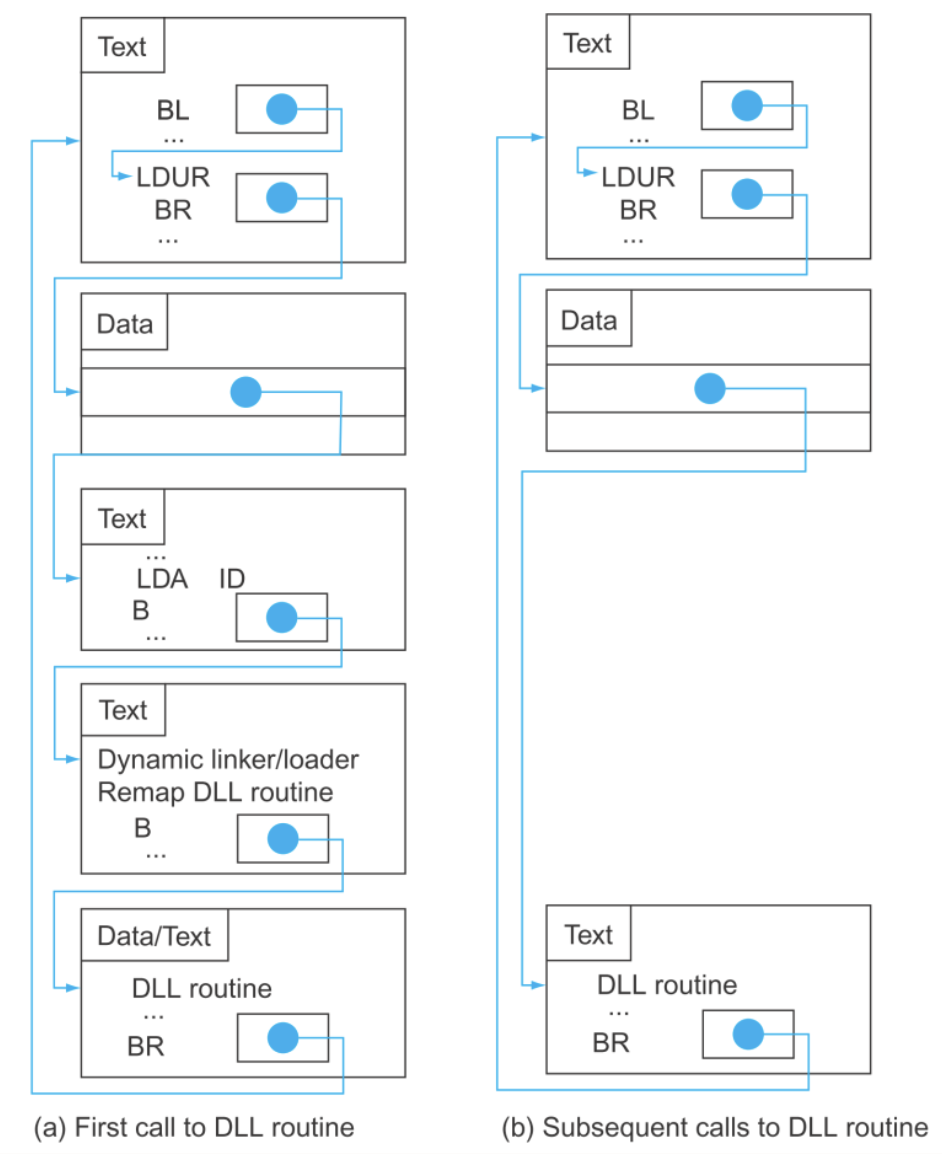
\includegraphics[width=0.5\columnwidth]{img/DLL_routine.png}
\end{center}

\subsubsection{Esempio di ordinamento in C}
Procedura swap (leaf)
\begin{verbatim}
void swap(long long int v[ ], long long int k)
{
      long long int temp;
      temp = v[k];
      v[k] = v[k + 1];
      v[k + 1] = temp;
}
\end{verbatim}
v in X0, k in X1, temp in X9\\
In Assembly:
\begin{verbatim}
swap:
      LSL X10, X1, #3 // X10 = k * 8
      ADD X10, X0, X10  // X10 = indirizzo di v[k]
      LDUR X9, [X10, #0] // X9 = v[k]
      LDUR X11, [X10, #8] // X11 = v[k+1]
      STUR X11, [X10, #0] // v[k] = X11
      STUR X9, [X10, #8] // v[k+1] = X9
      BL LR // Ritorna alla routine chiamante
\end{verbatim}

\Sep
\noindent
Procedura swap, non-leaf chiama swap
\begin{verbatim}
void swap(long long int v[ ], size_t n)
{
     size_t i, j;
      for( i = 0; i < n; i += 1)
      {
            for (j = i - 1; j >= 0 && v[j] > v[j+1]; j -= 1)
            {
                  swap(v, j);
            }
      }
}
\end{verbatim}
v in X0, n in X1, i in X19, j in X20\\
Scheletro del loop esterno:
\begin{verbatim}
      MOV X19,XZR // i = 0
      
for1tst:
      CMP X19, X1 // Compara X19 a X1 (i to n)
      B.GE exit1 // Vai a exit1 se X19 >= X1
      
       (body of outer for - loop)
       
       ADDI X19,X19,#1 // i += 1
       B for1tst // Vai al test del loop esterno
       
exit1:
\end{verbatim}

\Sep \noindent
Scheletro del loop interno:
\begin{verbatim}
      SUBI X10, X19, #1 // j = i - 1
      
for2tst:
      CMP X20, XZR // Compara X20 a 0
      B.LT exit2 // Vai a exit2 se X20 < 0
      LSL X10, X20, #3 // Reg X10 = j * 8
      ADD X11, X0, X10 // Reg X11 = v + (j * 8)
      LDUR X12, [X11, #0] // Reg X12 = v[j]
      LDUR X13, [X11, #8] // Reg X13 = v[j+1]
      CMP X12, X13 // Compara X12 a X13
      B.LE exit2 // Vai a exit2 se X12 <= X13
      MOV X0, X21 // Primo parametro di swap è v
      MOV X1, X20 // Secondo parametro di swap è j
      BL swap // Chiama la funzione swap
      MOV X1, X22 // Necessario per la comparazione nel primo loop
      SUBI X20, X20, #1 // j -= 1
      B for2tst // Vai al test del loop interno
      
exit2:
\end{verbatim}

\Sep \noindent
Preserva i registri salvati:
\begin{verbatim}
      SUBI SP, SP #40 // Crea lo spazio sullo stack pointer per 5 registri
      STUR LR, [SP, #32] // Salva LR sullo stack
      STUR X22, [SP, #24] // Salva X22 sullo stack
      STUR X21, [SP, #16] // Salva X21 sullo stack
      STUR X20, [SP, #8] // Salva X20 sullo stack
      STUR X19, [SP, #0] // Salva X19 sullo stack
      MOV X21, X0 // Copia il parametro X0 in X21
      MOV X22, X1 // Copia il parametro X1 in X22
\end{verbatim}

\Sep \noindent
Ripristino dei registri salvati:
\begin{verbatim}
exit1:
      LDUR X19, [SP, #0] // Ripristino di X19 dallo stack
      LDUR X20, [SP, #8] // Ripristino di X20 dallo stack
      LDUR X21, [SP, #16] // Ripristino di X21 dallo stack
      LDUR X22, [SP, #24] // Ripristino di X22 dallo stack
      LDUR X30, [SP, #32] // Ripristino LR dallo stack
      ADDI SP, SP, #40 // Ripristino stack pointer
\end{verbatim}

\subsection{Array vs Puntatori}
L'indicizzazione degli array comporta:
\begin{itemize}
\item Moltiplicare l'indice per dimensione dell'elemento
\item Aggiunta all'indirizzo di base dell'array
\end{itemize}
I puntatori corrispondono direttamente agli indirizzi di memoria:
\begin{itemize}
\item Può evitare la complessità dell'indicizzazione
\end{itemize}

\begin{center}
\begin{tabular}{|l|l|}
\hline
\begin{minipage}{.5\linewidth}
\begin{verbatim}

 clear1(int array[], int size)
 {
int i;
for(i = 0; i < size; i += 1)
       array[i] = 0;
 }
 
\end{verbatim}
\end{minipage} & 
\begin{minipage}{.5\linewidth}
\begin{verbatim}

 clear2(int *array, int size)
 {
int *p;
for(p=&array[0]; p<&array[size]; p++)
      *p = 0;
 }
 
\end{verbatim}
\end{minipage}\\ \hline
\begin{minipage}{.5\linewidth}
\begin{verbatim}

MOV X9, XZR // i = 0
      
loop1:
LSL X10, X9, #3 // X10 = i * 8
ADD X11, X0, X10 // X11 = indirizzo
                // di array[i]
STUR XZR, [X11, #0] // array[i] = 0
ADDI X9, X9, #1 // i += 1
CMP X9, X1 // Compara i a size
B.LT loop1 // Se i < size vai a loop1

\end{verbatim}
\end{minipage} &
\begin{minipage}{.5\linewidth}
\begin{verbatim}

MOV X9, X0 // p=indirizzo di array[0]
LSL X10, X1, #3 // X10 = size * 8
ADD X11, X0, X10 // X11 = indirizzo
                // di array[size]
      
loop2:
STUR XZR, [X9, #0] // Memory[p] = 0
ADDI X9, X9, #8 // p += 8
CMP X9,X11 // Compara p a &array[size]
B.LT loop2 // Se minore vai a loop2

\end{verbatim}
\end{minipage}\\ \hline
\end{tabular}
\end{center}
La versione array richiede che lo spostamento sia all'interno del ciclo
\begin{itemize}
\item Parte del calcolo dell'indice per incrementare i
\item Puntatore incrementante c.f.
\end{itemize}
Il compilatore può ottenere lo stesso effetto dell'uso manuale dei puntatori
\begin{itemize}
\item Eliminazione della variabile di induzione
\item Meglio rendere il programma più chiaro e sicuro
\end{itemize}

\subsection{Istruzioni ARMv7 (32-bit)}
In piedi originariamente per la Acorn RISC Machine, in seguito cambiata in Advanced RISC Machine.\\
ARMv1 è uscito nel 1985 con indirizzi a 32 bit. Molte versioni del set di istruzioni ARM a 32 bit sono uscite nel corso degli anni, culminando con ARMv7 nel 2005.
ARMv8 con indirizzi a 64 bit è stato rivelato nel 2013, con grandi differenze.\\
Somiglianze tra ARMv7 e ARMv8:
\begin{itemize}
\item Tutte le istruzioni sono larghe 32 bit per entrambe le architetture.
\item L'unico modo per accedere alla memoria è tramite istruzioni di caricamento e archiviazione su entrambe le architetture.
\end{itemize}
Ma ecco alcune delle differenze:
\begin{itemize}
\item ARMv7 e i precedenti set di istruzioni ARM hanno solo 15 registri generici.
\item Nessun registro è cablato a 0, quindi ARMv7 e i suoi predecessori hanno bisogno di istruzioni extra per eseguire alcune operazioni che ARMv8 può fare con XZR.
\item Il 16esimo registro mancante in ARMv7 e nei suoi predecessori è il program counter (PC).
\item Le modalità di indirizzamento ARMv7 non funzionano per tutte le dimensioni dei dati.
\item ARMv7 ha istruzioni Load Multiple e Store Multiple. ARMv8 no.
\item Piuttosto che il campo immediato è semplicemente una costante, è essenzialmente un input per una funzione che produce una costante. Gli otto campi immediati a bit minimi sono estesi a zero a valore a 32 bit e poi ruotato a destra il numero di bit specificato nei primi quattro bit del campo moltiplicato per due.
\item A differenza di ARMv8, i primi set di istruzioni ARM hanno omesso un'istruzione divide.
\end{itemize}

\subsection{Il resto del set di istruzioni ARMv8}
\Sep
\begin{center}
\begin{tabular}{|c|cc|cc|cc|cc|}
\hline
\rowcolor[HTML]{FFCB2F} 
Classe                          & \multicolumn{2}{c|}{\cellcolor[HTML]{FFCB2F}Loads / Stores} & \multicolumn{2}{c|}{\cellcolor[HTML]{FFCB2F}Operazioni} & \multicolumn{2}{c|}{\cellcolor[HTML]{FFCB2F}Branches} & \multicolumn{2}{c|}{\cellcolor[HTML]{FFCB2F}Totale} \\ \hline
                                & \multicolumn{1}{c|}{AL}                & ML                 & \multicolumn{1}{c|}{AL}               & ML              & \multicolumn{1}{c|}{AL}              & ML             & \multicolumn{1}{c|}{AL}            & ML             \\ \hline
Intero                          & \multicolumn{1}{c|}{49}                & 145                & \multicolumn{1}{c|}{74}               & 105             & \multicolumn{1}{c|}{-}               & -              & \multicolumn{1}{c|}{123}           & 250            \\ \hline
Floating Point \& Int Mul / Div & \multicolumn{1}{c|}{0}                 & 18                 & \multicolumn{1}{c|}{63}               & 156             & \multicolumn{1}{c|}{-}               & -              & \multicolumn{1}{c|}{63}            & 174            \\ \hline
SIMD / Vector                   & \multicolumn{1}{c|}{16}                & 166                & \multicolumn{1}{c|}{229}              & 371             & \multicolumn{1}{c|}{-}               & -              & \multicolumn{1}{c|}{245}           & 537            \\ \hline
Sistema / Speciali              & \multicolumn{1}{c|}{11}                & 55                 & \multicolumn{1}{c|}{}                 &                 & \multicolumn{1}{c|}{-}               & -              & \multicolumn{1}{c|}{63}            & 95             \\ \hline
                                & \multicolumn{1}{c|}{-}                 & -                  & \multicolumn{1}{c|}{-}                & -               & \multicolumn{1}{c|}{23}              & 14             & \multicolumn{1}{c|}{23}            & 14             \\ \hline
Totale                          & \multicolumn{1}{c|}{76}                & 384                & \multicolumn{1}{c|}{418}              & 672             & \multicolumn{1}{c|}{23}              & 14             & \multicolumn{1}{c|}{517}           & 1070           \\ \hline
\end{tabular}
\end{center}
Molte istruzioni di assemblaggio vengono tradotte in diverse istruzioni della macchina (ad esempio opcode) in base ai dati su cui operano.\\
ARMv8 include entrambe le versioni a 32 bit e 64 bit delle istruzioni all'interno della stessa architettura.\\
In linguaggio assembly, i programmatori utilizzano registri nominati W0, W1, \dots al posto di X0, X1, \dots per specificare le operazioni a 32 bit.
\begin{center}
\begin{minipage}{.2\textwidth}
\begin{verbatim}
ADD X9, X21, X9

ADD W9, W21, W9
\end{verbatim}
\end{minipage}
\end{center}
Dalla panoramica del set di istruzioni ARMv8:
\begin{itemize}
\item La maggior parte delle istruzioni intere nel set di istruzioni A64 ha due forme, che operano su valori a 32 o 64 bit all'interno del file di registro generico a 64 bit.
\item Quando viene selezionato un modulo di istruzioni a 32 bit, vale quanto segue:
\begin{itemize}
\item I 32 bit superiori dei registri sorgente vengono ignorati;
\item I 32 bit superiori del registro di destinazione sono impostati su ZERO;
\item Gli spostamenti/rotati a destra iniettano al bit 31, invece del bit 63;
\item I flag delle condizioni, dove impostati dall'istruzione, vengono calcolati dai 32 bit inferiori.
\end{itemize}
\end{itemize}

\subsubsection{ARMv8 Istruzioni logiche aritmetiche intere}
Grassetto significa che l'istruzione è anche in LEGv8, corsivo significa che è una pseudoistruzione, e grassetto corsivo significa che è una pseudoistruzione che è anche in LEGv8.
\begin{longtable}{|c|c|l|}
\hline
\rowcolor[HTML]{FFCB2F} 
\multicolumn{1}{|c|}{Tipo}                                        & \multicolumn{1}{c|}{Simbolo}     & \multicolumn{1}{c|}{Istruzione}                                \\ \hline
\endfirsthead
%
\multicolumn{3}{c}%
{{\bfseries Continua dalla pagina precedente}} \\
\hline
\rowcolor[HTML]{FFCB2F} 
\multicolumn{1}{|c|}{Tipo}                                        & \multicolumn{1}{c|}{Simbolo}     & \multicolumn{1}{c|}{Istruzione}                                \\ \hline
\endhead
                                                           & \textbf{ADD}          & Addizione                                          \\ \cline{2-3} 
                                                           & \textbf{ADDS}         & Addizione e set del flag                           \\ \cline{2-3} 
                                                           & \textbf{SUB}          & Sottrazione                                        \\ \cline{2-3} 
                                                           & \textbf{SUBS}         & Sottrazione e set del flag                         \\ \cline{2-3} 
                                                           & \textit{\textbf{CMP}} & Comparazione                                       \\ \cline{2-3} 
                                                           & \textit{CMN}          & Comparazione negativa                              \\ \cline{2-3} 
                                                           & \textit{NEG}          & Negazione                                          \\ \cline{2-3} 
\multirow{-8}{*}{Op. aritmetiche}                   & \textit{NEGS}         & Negazione e set del flag                           \\ \hline
                                                           & \textbf{ADDI}         & Addizione immediata                                \\ \cline{2-3} 
                                                           & \textbf{ADDIS}        & Addizione immediata e set del flag                 \\ \cline{2-3} 
                                                           & \textbf{SUBI}         & Sottrazione immediata                              \\ \cline{2-3} 
                                                           & \textbf{SUBIS}        & Sottrazione immediata e set del flag               \\ \cline{2-3} 
                                                           & \textbf{CMPI}         & Comparazione immediata                             \\ \cline{2-3} 
\multirow{-6}{*}{Op. aritmetiche immediate}         & \textit{CMNI}         & Comparazione negativa immediata                    \\ \hline
                                                           & ADD                   & Agiungi registro esteso                            \\ \cline{2-3} 
                                                           & ADDS                  & Agiungi registro esteso e setta il flag            \\ \cline{2-3} 
                                                           & SUB                   & Sottrae registro esteso                            \\ \cline{2-3} 
                                                           & SUBS                  & Sottrae registro esteso e setta il flag            \\ \cline{2-3} 
                                                           & \textit{CMP}          & Compara registro esteso                            \\ \cline{2-3} 
\multirow{-6}{*}{Aritmetica estesa}                        & \textit{CMN}          & Compara registro esteso negativo                   \\ \hline
                                                           & ADC                   & Addizione con carry                                \\ \cline{2-3} 
                                                           & ADCS                  & Addizione con carry e set del flag                 \\ \cline{2-3} 
                                                           & SBC                   & Sottrazione con carry                              \\ \cline{2-3} 
                                                           & SBCS                  & Sottrazione con carry e set del flag               \\ \cline{2-3} 
                                                           & \textit{NGC}          & Negazione con carry                                \\ \cline{2-3} 
\multirow{-6}{*}{Aritmerica con carry}                     & \textit{NGCS}         & Negazione con carry e set del flag                 \\ \hline
                                                           & \textbf{AND}          & AND bit a bit                                      \\ \cline{2-3} 
                                                           & \textbf{ANDS}         & AND bit a bit e set del flag                       \\ \cline{2-3} 
                                                           & \textbf{ORR}          & OR (inclusivo) bit a bit                           \\ \cline{2-3} 
                                                           & \textbf{EOR}          & OR (esclusivo) bit a bit                           \\ \cline{2-3} 
                                                           & BIC                   & Pulisce bit a bit                                  \\ \cline{2-3} 
                                                           & BICS                  & Puslice bit a bit e setta il flag                  \\ \cline{2-3} 
                                                           & ORN                   & OR NOT (inclusivo) bit a bit                       \\ \cline{2-3} 
                                                           & EON                   & OR NOT (esclusivo) bit a bit                       \\ \cline{2-3} 
                                                           & \textit{MVN}          & NOT bit a bit                                      \\ \cline{2-3} 
\multirow{-10}{*}{Op. logiche}                      & \textit{TST}          & Test bits                                          \\ \hline
                                                           & \textbf{ANDI}         & AND bit a bit immediato                            \\ \cline{2-3} 
                                                           & \textbf{ANDIS}        & AND bit a bit e set del flag immediato             \\ \cline{2-3} 
                                                           & \textbf{ORRI}         & OR (inclusivo) bit a bit immediato                 \\ \cline{2-3} 
                                                           & \textbf{EORI}         & OR (esclusivo) bit a bit immediato                 \\ \cline{2-3} 
\multirow{-5}{*}{Op. logiche immediate}             & \textit{TSTI}         & Test bits immediato                                \\ \hline
                                                           & \textbf{LSL}          & Shift logico a sx immediato                  \\ \cline{2-3} 
                                                           & \textbf{LSR}          & Shift logico a dx immediato                    \\ \cline{2-3} 
                                                           & ASR                   & Shift artimetico a dx immediato                \\ \cline{2-3} 
                                                           & ROR                   & Rotazione a dx immediata                       \\ \cline{2-3} 
                                                           & LSRV                  & Shift logico a dx del registro                 \\ \cline{2-3} 
                                                           & LSLV                  & Shift logico a sx del registro               \\ \cline{2-3} 
                                                           & ASRV                  & Shift artimetico a dx del registro             \\ \cline{2-3} 
\multirow{-8}{*}{Shift di registri}                        & RORV                  & Rotazione a dx del registro                    \\ \hline
                                                           & \textbf{MOVZ}         & Sposta registro con zero                           \\ \cline{2-3} 
                                                           & \textbf{MOVK}         & Sposta registro con keep                           \\ \cline{2-3} 
                                                           & MOVN                  & Sposta registro con NOT                            \\ \cline{2-3} 
\multirow{-4}{*}{Spostamento di registri}                  & \textit{\textbf{MOV}} & Sposta registro                                    \\ \hline
                                                           & BFM                   & Spost. campo di bit                       \\ \cline{2-3} 
                                                           & SBFM                  & Spost. campo di bit (segno)           \\ \cline{2-3} 
                                                           & UBFM                  & Spost. del campo di bit (senza segno)         \\ \cline{2-3} 
                                                           & BFI                   & Inserim. campo di bit (segno)           \\ \cline{2-3} 
                                                           & BFXIL                 & Estraz. campo di bit e ins. in basso \\ \cline{2-3} 
                                                           & SBFIZ                 & Campo bit con segno inserito in 0                  \\ \cline{2-3} 
                                                           & SBFX                  & Estraz. campo di bit (segno)            \\ \cline{2-3} 
                                                           & UBFIZ                 & Campo bit no segno inserito in 0                \\ \cline{2-3} 
                                                           & UBFX                  & Estraz. campo di bit (no segno)          \\ \cline{2-3} 
\multirow{-10}{*}{Inserim./Estraz. campo di bit} & EXTR                  & Estraz. di registro da una coppia               \\ \hline
                                                           & \textit{SXTB}         & Byte di estensione del segno                       \\ \cline{2-3} 
                                                           & \textit{SXTH}         & Halfword di estensione del segno                   \\ \cline{2-3} 
                                                           & \textit{SXTW}         & Word di estensione del segno                       \\ \cline{2-3} 
                                                           & \textit{UXTB}         & Byte di estensione senza segno                     \\ \cline{2-3} 
\multirow{-5}{*}{Estensione del segno}                     & \textit{UXTH}         & Halfword di estensione senza segno                 \\ \hline
                                                           & CLS                   & Conta i bit del segno iniziale                     \\ \cline{2-3} 
                                                           & CLZ                   & Conta i bit con 0 iniziale                         \\ \cline{2-3} 
                                                           & RBIT                  & Inverte l'ordine dei bit                           \\ \cline{2-3} 
                                                           & REV                   & Inverte i byte nel registro                        \\ \cline{2-3} 
                                                           & REV16                 & Inverte i byte nelle halfword                      \\ \cline{2-3} 
\multirow{-6}{*}{Operazioni di bit}                        & REV32                 & Inverte i byte nelle word                          \\ \hline
\end{longtable}
Il secondo registro di tutte le operazioni di elaborazione aritmetica e logica ha la possibilità di essere spostato prima di essere utilizzato. Le opzioni di spostamento sono spostamento a sinistra logico, spostamento a destra logico, spostamento aritmetico destro e rotazione a destra. Sebbene l'assembler abbia istruzioni esplicite con questi nomi (LSL, LSR, SRA e ROR), queste sono in realtà solo pseudoistruzioni.\\
Per supportare l'aritmetica sui tipi di dati più ristretti, ci sono istruzioni che ti consentono di mescolare le dimensioni dei dati del secondo operando per segno che lo estende o zero estendendolo fino all'intera larghezza. Le istruzioni del registro esteso funzionano con byte, halfword o word.\\
Per supportare le operazioni di aggiunta e sottrazione su operandi più grandi di una doubleword, ARM include istruzioni per aggiungere o sottrarre il trasporto da un'operazione precedente. ASR fa lo spostamento aritmetico a destra, che replica il bit del segno durante lo spostamento, e ROR ruota i bit a destra; cioè, i bit spostati a destra vengono inseriti a sinistra.\\
Ci sono versioni di tutte le istruzioni di turno che determinano l'importo da spostare in base a un valore in un registro piuttosto che come immediato all'interno dell'istruzione. Per manipolare i campi di bit, il set completo di istruzioni ARMv8 include istruzioni che possono estrarre un campo bit da un registro e inserirlo in un altro.


\subsubsection{ARMv8 Istruzioni per il trasferimento dati}
Non abbiamo visto tutte le modalità di indirizzamento disponibili, solo l'offset immediato non scalato.
Eccone altri cinque:
\begin{enumerate}
\item Base più un offset immediato senza segno a 12 bit scalato.
\item Base più un offset del registro a 64 bit, opzionalmente scalato.
\item Base più un offset del registro esteso a 32 bit, opzionalmente scalato.
\end{enumerate}
Le opzioni di ridimensionamento delle prime tre modalità di indirizzamento moltiplicano o ridimensionano l'indirizzo nel campo immediato o nel registro per la dimensione dei dati trasferiti in byte.\\
Quindi, se X11 contiene $100.000_{ten}$
\begin{verbatim}
LDR X10, [X11, #16] // Modalità di scala
\end{verbatim}
Caricherà la doppia parola (8 byte) all'indirizzo $100.128_{ten}$ (100.000 + 8*16) nel registro X10.\\
L'indirizzo della seconda modalità di indirizzamento è semplicemente la somma di due registri, con l'opzione di spostamento del secondo operando di 1, 2 o 3 bit.\\
Se X11 contiene $100.000_{ten}$ e X12 contiene $1.000_{ten}$
\begin{verbatim}
LDR X10, [X11, X12 LSL #3] // Base + registro scalato
\end{verbatim}
Caricherà il doppio all'indirizzo $108.000_{ten}$ (100.000 + 2 3 *1000) nel registro X10.\\
La terza modalità di indirizzamento utilizza semplicemente un registro a 32 bit (ad esempio, W12) invece di un registro a 64 bit
\begin{enumerate}\setcounter{enumi}{3}
\item Pre-indicizzato da un offset immediato firmato a 9 bit non scalato.
\item Post-indicizzato da un offset immediato firmato a 9 bit non scalato.
\end{enumerate}
Queste ultime due modalità di indirizzamento cambiano il registro di base come parte del calcolo dell'indirizzo.\\
Quindi, se X11 contiene $100.000_{ten}$

\begin{verbatim}
LDR X10, [X11, #16]! // modalità di pre-indicizzamento dell'indirizzo
\end{verbatim}
Carica la doubleword all'indirizzo $100.016_{ten}$ nel registro X10 e cambierà X11 in $100.016_{ten}$.
\begin{verbatim}
LDR X10, [X11], #16 // modalità di post-indicizzamento dell'indirizzo
\end{verbatim}
Carica la doubleword all'indirizzo $100.000_{ten}$ nel registro X10 e cambierà X11 in $100.016_{ten}$.\\
Tra le altre cose, per accelerare i trasferimenti di dati, ARMv8 include tre istruzioni load pair e store pair (LDP, LDPSW, STP), che trasferiscono due doubleword alla volta.

\begin{center}
\begin{tabular}{|c|c|c|}
\hline
\rowcolor[HTML]{FFCB2F} 
Tipo                                                                                                         & Simbolo         & Istruzione                                                                                                \\ \hline
                                                                                                             & \textbf{LDUR}   & Carica registro                                                                                           \\ \cline{2-3} 
                                                                                                             & \textbf{LDURB}  & Carica byte                                                                                               \\ \cline{2-3} 
                                                                                                             & LDURSB          & Carica byte (con segno)                                                                                   \\ \cline{2-3} 
                                                                                                             & \textbf{LDURH}  & Carica halfword                                                                                           \\ \cline{2-3} 
                                                                                                             & LDURSH          & Carica halfword (con segno)                                                                               \\ \cline{2-3} 
                                                                                                             & \textbf{LDURSW} & Carica word (con segno)                                                                                   \\ \cline{2-3} 
                                                                                                             & \textbf{STUR}   & Store registro                                                                                            \\ \cline{2-3} 
                                                                                                             & \textbf{STURB}  & Store byte                                                                                                \\ \cline{2-3} 
                                                                                                             & \textbf{STURH}  & Store halfword                                                                                            \\ \cline{2-3} 
                                                                                                             & \textbf{STURW}  & Store word                                                                                                \\ \cline{2-3} 
\multirow{-11}{*}{Unscaled}                                                                                  & \textbf{LDA}    & Carica indirizzo                                                                                          \\ \hline
                                                                                                             & LDR             & Carica registro                                                                                           \\ \cline{2-3} 
                                                                                                             & LDRB            & Carica byte                                                                                               \\ \cline{2-3} 
                                                                                                             & LDRSB           & Carica byte (con segno)                                                                                   \\ \cline{2-3} 
                                                                                                             & LDRH            & Carica halfword                                                                                           \\ \cline{2-3} 
                                                                                                             & LDRSH           & Carica halfword (con segno)                                                                               \\ \cline{2-3} 
                                                                                                             & LDRSW           & Carica word (con segno)                                                                                   \\ \cline{2-3} 
                                                                                                             & STR             & Store registro                                                                                            \\ \cline{2-3} 
                                                                                                             & STRB            & Store byte                                                                                                \\ \cline{2-3} 
\multirow{-9}{*}{\begin{tabular}[c]{@{}c@{}}Scaled\\ Extended\\ Pre \& Post Indexed\end{tabular}}            & STRH            & Store halfword                                                                                            \\ \hline
                                                                                                             & \textbf{LDXR}   & Load esclusivo registro                                                                                   \\ \cline{2-3} 
                                                                                                             & LDXRB           & Load esclusivo byte                                                                                       \\ \cline{2-3} 
                                                                                                             & LDXRH           & Load esclusivo halfword                                                                                   \\ \cline{2-3} 
                                                                                                             & LDXP            & Load esclusivo pair                                                                                       \\ \cline{2-3} 
                                                                                                             & \textbf{STXR}   & Store esclusivo registro                                                                                  \\ \cline{2-3} 
                                                                                                             & STXRB           & Store esclusivo byte                                                                                      \\ \cline{2-3} 
                                                                                                             & STXRH           & Store esclusivo halfword                                                                                  \\ \cline{2-3} 
                                                                                                             & STXP            & Store esclusivo pair                                                                                      \\ \cline{2-3} 
                                                                                                             & LDAXR           & Load-aquire registri eslusivo                                                                             \\ \cline{2-3} 
                                                                                                             & LDAXRB          & Load-aquire byte eslusivo                                                                                 \\ \cline{2-3} 
                                                                                                             & LDAXRH          & Load-aquire halfword eslusivo                                                                             \\ \cline{2-3} 
                                                                                                             & LDAXP           & Load-aquire pair eslusivo                                                                                 \\ \cline{2-3} 
                                                                                                             & STLXR           & Store-release registri esclusivo                                                                          \\ \cline{2-3} 
                                                                                                             & STLXRB          & Store-release byte esclusivo                                                                              \\ \cline{2-3} 
                                                                                                             & STLXRH          & Store-release halfword esclusivo                                                                          \\ \cline{2-3} 
                                                                                                             & STLXP           & Store-release pair esclusivo                                                                              \\ \cline{2-3} 
                                                                                                             & LDP             & Load pair                                                                                                 \\ \cline{2-3} 
                                                                                                             & LDPSW           & Load pair (con segno)                                                                                     \\ \cline{2-3} 
                                                                                                             & STP             & Store pair                                                                                                \\ \cline{2-3} 
                                                                                                             & ADRP            & Calcola l'indirizzo di una pagina da 4 KB \\ \cline{2-3} 
\multirow{-21}{*}{\begin{tabular}[c]{@{}c@{}}PC\\ Pair\\ Exclusive\\ Exclusive Acquire/Release\end{tabular}} & ADR             & Calcola l'indirizzo della label                                                      \\ \hline
\end{tabular}
\end{center}


\subsection{ARMv8 Istruzioni di Branch}
\Sep
\begin{center}
\begin{tabular}{|c|c|c|}
\hline
\rowcolor[HTML]{FFCB2F} 
Tipo                                                                                                         & Simbolo         & Istruzione                                                                                                \\ \hline
                                                                                                             & \textbf{B.cond} & Salto condizionale                                                                                        \\ \cline{2-3} 
                                                                                                             & \textbf{CBNZ}   & Compara e salta se non zero                                                                               \\ \cline{2-3} 
                                                                                                             & \textbf{CBZ}    & Compara e salta se zero                                                                                   \\ \cline{2-3} 
                                                                                                             & TBNZ            & Testa e salta se non zero                                                                                 \\ \cline{2-3} 
\multirow{-5}{*}{Salti condizionali}                                                                         & TBZ             & Testa e salta se zero                                                                                     \\ \hline
                                                                                                             & \textbf{B}      & Salto senza condizioni                                                                                    \\ \cline{2-3} 
                                                                                                             & \textbf{BL}     & Salta a un link                                                                                           \\ \cline{2-3} 
                                                                                                             & BLR             & Salta a un link a un registro                                                                             \\ \cline{2-3} 
                                                                                                             & \textbf{BR}     & Salta a un registro                                                                                       \\ \cline{2-3} 
\multirow{-5}{*}{Salti non condizionali}                                                                     & RET             & Ritorna alla subroutine                                                                                   \\ \hline
                                                                                                             & CSEL            & Selezione condizionale                                                                                    \\ \cline{2-3} 
                                                                                                             & CSINC           & Selezione condizionale dell'incremento                                                                    \\ \cline{2-3} 
                                                                                                             & CSINV           & Selezione condiizonale dell'inverso                                                                       \\ \cline{2-3} 
                                                                                                             & CSNEG           & Selezione condizionale del negato                                                                         \\ \cline{2-3} 
                                                                                                             & \textit{CSET}   & Set condizionale                                                                                          \\ \cline{2-3} 
                                                                                                             & \textit{CSETM}  & Set mask condizionale                                                                                     \\ \cline{2-3} 
                                                                                                             & \textit{CINC}   & Incremento condizionale                                                                                   \\ \cline{2-3} 
                                                                                                             & \textit{CINV}   & Inversione condizionale                                                                                   \\ \cline{2-3} 
\multirow{-9}{*}{Selezioni condizionali}                                                                     & \textit{CNEG}   & Negazione condizionale                                                                                    \\ \hline
                                                                                                             & CCMP            & Compare tra registri condizionale                                                                    \\ \cline{2-3} 
                                                                                                             & CCMPI           & Compare immediata condizionale                                                                       \\ \cline{2-3} 
                                                                                                             & CCMN            & Compare tra registri negativi condizionale                                                           \\ \cline{2-3} 
\multirow{-4}{*}{Comparazioni condizionali}                                                                  & CCMNI           & Compare immediata negativa condizionale                                                              \\ \hline
\end{tabular}
\end{center}
Ci sono altri due salti incondizionati:
\begin{itemize}
\item Il primo è una variazione di ramo e link che utilizza un registro per l'indirizzo della filiale (BALR). 
\item Il secondo è il ritorno dalla subroutine (RET), che suona molto simile al registro delle filiali (BR);
\end{itemize}
Il motivo per cui ARMv8 ha diversi opcode per la stessa operazione è che i predittori di salti hardware possano sapere se è davvero di ritorno da una subroutine (RET), che è facile da prevedere, o di essere utilizzato in una tabella di rami (BR), che è molto più difficile da prevedere.\\
Ci sono istruzioni che memorizzano un valore in un registro basato sui codici delle condizioni. L'idea alla base delle istruzioni di selezione delle condizioni è quella di sostituire i salti condizionali, che possono causare problemi all'esecuzione delle pipeline se non possono essere predetti.

\subsection{Errori}
\begin{itemize}
\item Istruzioni potenti $\Rightarrow$ Performance migliori\\
Meno istruzioni richieste ma le istruzioni complesse sono difficili da implementare. Può rallentare tutte le istruzioni, comprese quelle semplici. I compilatori sono bravi a creare codice veloce da semplici istruzioni
\item Usa il codice di assemblaggio per prestazioni elevate\\
I compilatori moderni sono più bravi a trattare con i processori moderni. Più righe di codice $\Rightarrow$ più errori e meno produttività
\item Compatibilità all'indietro $\Rightarrow$ il set istruzioni non cambia\\
Ma accumulano più istruzioni
\begin{center}
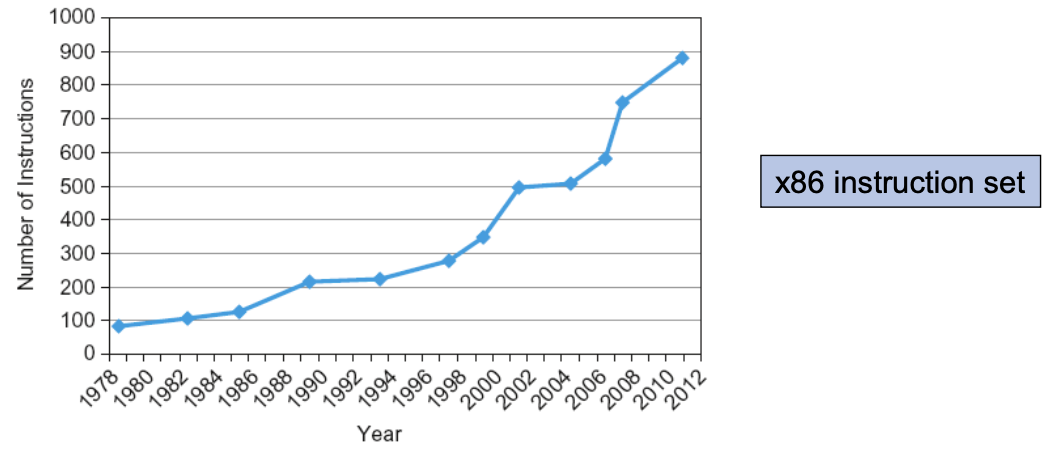
\includegraphics[width=0.5\columnwidth]{img/istruzioni_x86.png}
\end{center}
\end{itemize}

\subsection{Insidie}
\begin{itemize}
\item Le parole sequenziali non sono agli indirizzi sequenziali: Incremento di 4, non di 1!
\item Mantenere un puntatore a una variabile automatica dopo i ritorni della procedura\\
Ad esempio, passando il puntatore indietro tramite un argomento. Il puntatore diventa invalido quando lo stack viene svuotato
\end{itemize}

%CAPITOLO 3
\clearpage
\section{Aritmetic in LEGv8}
\subsection{Moltiplicazione in LEGv8}
Per produrre un prodotto a 128 bit correttamente firmato o non firmato, LEGv8 ha tre istruzioni:
\begin{itemize}
\item Moltiplicazione (\textbf{MUL})
\item Moltiplicazione con segno alto (\textbf{SMULH})
\item Moltiplicazione senza segno alto (\textbf{UMULH}).
\end{itemize}
Per ottenere il prodotto intero a 64 bit, il programmatore utilizza MUL. Per ottenere i 64 bit superiori del prodotto a 128 bit, il programmatore utilizza SMULH o UMULH, a seconda dei tipi di moltiplicatore e moltiplicatore.\\
Le istruzioni di moltiplicazione LEGv8 non impostano il codice delle condizioni di overflow, quindi spetta al software verificare se il prodotto è troppo grande per adattarsi a 64 bit. Non c'è overflow se i 64 bit superiori sono 0 per UMULH o il segno replicato dei 64 bit inferiori per SMULH.

\subsection{Divisione in LEGv8}
Per gestire sia numeri interi firmati che numeri interi non firmati, LEGv8 ha due istruzioni:
\begin{itemize}
\item Divisione con segno (\textbf{SDIV})
\item Divisione senza segno (\textbf{UDIV})
\end{itemize}
Il supporto hardware comune per moltiplicare e dividere consente a LEGv8 di fornire una singola coppia di registri a 64 bit che vengono utilizzati sia per moltiplicare che per dividere. Le istruzioni LEGv8 divide ignorano l'overflow: il software deve determinare se il quoziente è troppo grande. Oltre all'overflow, la divisione può anche comportare un calcolo improprio: divisione per 0. \textsl{Il software LEGv8 deve controllare il divisore per scoprire la divisione per 0 e l'overflow}.

\begin{center}
\begin{tabular}{|l|l|l|}
\hline
Moltiplicazione & MUL X1, X2, X3 & X1 = X2 * X3\\ \hline
Moltiplicazione con segno alto & SMULH X1, X2, X3 & X1 = X2 * X3\\ \hline
Moltiplicazione senza segno alto & UMULH X1, X2, X3 & X1 = X2 * X3\\ \hline
Divisione con segno & SDIV X1, X2, X3 & X1 = X2 / X3\\ \hline
Divisione senza segno & UDIV X1, X2, X3 & X1 = X2 / X3\\ \hline
\end{tabular}
\end{center}

\subsection{Floating Point}
Rappresentanza per i numeri non interi, compresi numeri molto piccoli e molto grandi. Un esempio di notazione floating point è la notazione scientifica
\begin{itemize}
\item Normalizzato: $-2,34 \cdot 10^{56}$
\item Non normalizzato: $+0,002 \cdot 10^{-4}$ oppure $+987,02 \cdot 10^9$
\end{itemize}
In binario:
$$ \pm 1.xxxxxxx_2 \cdot 2^{yyyy}$$
Dei tipi floating point in C sono le variabili float e double

\subsubsection{Floating Point Standard IEEE Std 754-1985}
Due rappresentazioni: precisione singola (32 bit) e doppia precisione (64 bit)
\begin{center}
\begin{tabular}{ccc}
 & singola: 8 bits & singola: 23 bits\\
 & double: 11 bits & double 52 bits\\ \hline
 \multicolumn{1}{|c|}{S} & \multicolumn{1}{c|}{Esponente} & \multicolumn{1}{c|}{Frazione}\\ \hline
\end{tabular}
\end{center}
$$x = (-1)^S \times (1+Frazione) \times 2^{Esponente - Bias}$$
S: bit di segno (0 $\Rightarrow$ non negativo, 1 $\Rightarrow$ negativo)\\
Normalizzazione della parte significante: $1.0 \leq |parte\ significativa| < 2.0$
Ha sempre un 1 bit pre-punto binario iniziale, quindi non c'è bisogno di rappresentarlo esplicitamente (bit nascosto).\\
Esponente: rappresentazione in eccesso: esponente effettivo + Bias
\begin{itemize}
\item Assicura che l'esponente sia senza segno
\item Singola precisione: Bias = 127; Doppia precisione: Bias = 1023
\end{itemize}

\subsubsection{Range in singola precisione}
Esponenti 00000000 e 11111111 riservati
Valore più piccolo:
\begin{itemize}
\item Esponente: 00000001\\
	$\Rightarrow $ Esponente effettivo = 1 – 127 = –126
\item Frazione: 000...00 $\Rightarrow$ significa = 1,0
\item $\pm 1.0 \times 2^{-126} \approx \pm 1.2 \times 10^{-38}$
\end{itemize}
Valore più grande:
\begin{itemize}
\item Esponente: 11111110\\
	$\Rightarrow $ Esponente effettivo = 254 – 127 = +127
\item Frazione: 111...11 $\Rightarrow$ significa $\approx$ 2,0
\item $\pm 2.0 \times 2^{127} \approx \pm 3.4 \times 10^{+38}$
\end{itemize}

\subsubsection{Range in doppia precisione}
Esponenti 00000000 e 11111111 riservati
Valore più piccolo:
\begin{itemize}
\item Esponente: 00000000001\\
	$\Rightarrow $ Esponente effettivo = 1 – 1023 = –1022
\item Frazione: 000...00 $\Rightarrow$ significa = 1,0
\item $\pm 1.0 \times 2^{-1022} \approx \pm 2.2 \times 10^{-308}$
\end{itemize}
Valore più grande:
\begin{itemize}
\item Esponente: 11111111110\\
	$\Rightarrow $ Esponente effettivo = 2046 – 1023 = +1023
\item Frazione: 111...11 $\Rightarrow$ significa $\approx$ 2,0
\item $\pm 2.0 \times 2^{1023} \approx \pm 1.8 \times 10^{308}$
\end{itemize}

\subsubsection{Infiniti e NaNs}
Esponente = 111...1 e Frazione = 000...0
\begin{itemize}
\item $\pm$ Infinito
\item Può essere utilizzato nei calcoli successivi, evitando la necessità di controllo dell'overflow
\end{itemize}
 Esponente = 111...1 e Frazione $\not =$ 000...0
\begin{itemize}
\item Non un numero (NaN)
\item Indica un risultato illegale o indefinito
\item Ad esempio, $0 \over 0$
\item Può essere utilizzato nei calcoli successivi
\end{itemize}

\subsubsection{Numeri denormalizzati}
Esponente = 000...0 $\Rightarrow$ Il bit nascosto è 0
$$x = (-1)^S\times (0+Frazione)\times 2^{-Bias}$$
Più piccoli dei numeri normali. Consente un sottoflusso graduale, con precisione decrescente. Denormalizzazione con frazione = 000...0
$$x=(-1)^S\times (0+0)\times 2^{-Bias} = \pm 0.0$$
Notiamo che abbiamo due rappresentazione dello 0

\subsubsection{Riassunti IEEE Std 754-1985}
\Sep
\begin {center}
\begin{tabular}{|cc|cc|c|}
\hline
\rowcolor[HTML]{FFCB2F} 
\multicolumn{2}{|c|}{\cellcolor[HTML]{FFCB2F}Precisione singola} & \multicolumn{2}{c|}{\cellcolor[HTML]{FFCB2F}Precisione doppia} & Oggetto rappresentato       \\ \hline
\multicolumn{1}{|c|}{Esponente}            & Frazione            & \multicolumn{1}{c|}{Esponente}           & Frazione            &                             \\ \hline
\multicolumn{1}{|c|}{0}                    & 0                   & \multicolumn{1}{c|}{0}                   & 0                   & 0                           \\ \hline
\multicolumn{1}{|c|}{0}                    & Non zero            & \multicolumn{1}{c|}{0}                   & Non zero            & $\pm$ Numero denormalizzato \\ \hline
\multicolumn{1}{|c|}{1 - 254}              & Qualsiasi           & \multicolumn{1}{c|}{1 - 2046}            & Qualsiasi           & $\pm$ Numero floating point \\ \hline
\multicolumn{1}{|c|}{255}                  & 0                   & \multicolumn{1}{c|}{2047}                & 0                   & $\pm$ Infinito              \\ \hline
\multicolumn{1}{|c|}{255}                  & Non zero            & \multicolumn{1}{c|}{2047}                & Non zero            & NaN (Non a Number)          \\ \hline
\end{tabular}
\end{center}

\subsection{Overflow \& Underflow}
Per quanto riguarda le operazioni intere, l'operazione aritmetica in virgola mobile può originare "trabocchi". Overflow qui significa che l'esponente è troppo grande per essere rappresentato nel campo esponente.\\
Anche il virgola mobile offre un nuovo tipo di evento eccezionale: la frazione diversa da zero che stiamo calcolando potrebbe diventare così piccola che non può essere rappresentata. Chiamiamo questo evento underflow: si verifica quando l'esponente negativo è troppo grande per adattarsi al campo dell'esponente.

\subsubsection{Managing overflows and underflows}
Cosa dovrebbe accadere su un overflow o underflow per far sapere all'utente che si è verificato un problema?\\
LEGv8 può sollevare un'eccezione, chiamata anche interrupt su molti computer. Un'eccezione o un'interruzione è essenzialmente una chiamata di procedura non programmata. L'indirizzo dell'istruzione in overflow viene salvato in un registro, e il computer salta a un indirizzo predefinito per invocare la routine appropriata per quell'eccezione.\\
In alcune situazioni il programma può continuare dopo l'esecuzione del codice correttivo.

\subsection{Istruzioni Floating-Point in LEGv8}
LEGv8 supporta i formati IEEE 754 a precisione singola e doppia precisione con queste istruzioni:
\begin{itemize}
\item Aggiunta in virgola mobile, singola (\textbf{FADDS}) e addizione, doppia (\textbf{FADDD})
\item Sottrazione in virgola mobile, singola (\textbf{FSUBS}) e sottrazione, doppia (\textbf{FSUBD})
\item Moltiplicazione in virgola mobile, singola (\textbf{FMULS}) e moltiplicazione, doppia (\textbf{FMULD})
\item Divisione in virgola mobile, singola (\textbf{FDIVS}) e divisione, doppia (\textbf{FDIVD})
\item Confronto in virgola mobile, singola (\textbf{FCMPS}) e confronto, doppia (\textbf{FCMPD})
\end{itemize}
Registri separati in virgola mobile:
\begin{itemize}
\item vengono chiamati S0, S1, S2, ... per precisione singola e D0, D1, D2, . . . per doppia precisione.
\item I registri in precisione singola sono solo la metà inferiore dei registri a doppia precisione.
\end{itemize}
Le istruzioni FP funzionano solo sui registri FP. I programmi generalmente non fanno operazioni intere sui dati FP, o viceversa. Più registri con un impatto minimo sulle dimensioni del codice.\\
Istruzioni per il load e lo store FP:
\begin{itemize}
\item \textbf{LDURS, LDURD}
\item \textbf{STURS, STURD}
\end{itemize}

\subsubsection{Floating-point in linguaggio Assembly}
\Sep
\begin{center}
\begin{tabular}{|l|l|l|l|}
\hline
\rowcolor[HTML]{FFCB2F} 
\multicolumn{1}{|c|}{Categoria}                             & \multicolumn{1}{c|}{Istruzione}         & \multicolumn{1}{c|}{Esempio}                  & \multicolumn{1}{c|}{Significato}                \\ \hline
                                      & ADD singola       & FADDS S2, S4, S6         & S2 = S4 + S6               \\ \cline{2-4} 
                                      & SUB singola     & FSUBS S2, S4, S6         & S2 = S4 - S6               \\ \cline{2-4} 
                                      & MUL singola & FMULS S2, S4, S6         & S2 = S4 * S6               \\ \cline{2-4} 
                                      & DIV singola       & FDIVS S2, S4, S6         & S2 = S4 / S6               \\ \cline{2-4} 
                                      & ADD doppia        & FADDD D2, D4, D6         & D2 = D4 + D6               \\ \cline{2-4} 
                                      & SUB doppia      & FSUBD D2, D4, D6         & D2 = D4 - D6               \\ \cline{2-4} 
                                      & MUL doppia  & FMULD D2, D4, D6         & D2 = D4 * D6               \\ \cline{2-4} 
\multirow{-8}{*}{Aritmetica}          & DIV doppia        & FDIVD D2, D4, D6         & D2 = D4 / D6               \\ \hline
                                      & CMP singola    & FCMPS S4, S6             & Test S4 vs S6              \\ \cline{2-4} 
\multirow{-2}{*}{Branch} & CMP doppia     & FCMPD D4, D6             & Test D4 vs D6              \\ \hline
                                      & Load singolo               & LDURS S1, {[}X23, 100{]} & S1 = Memory{[}X23 + 100{]} \\ \cline{2-4} 
                                      & Load doppio                & LDURD D1, {[}X23, 100{]} & D1 = Memory{[}X23 + 100{]} \\ \cline{2-4} 
                                      & Store singolo              & STURS S1, {[}X23, 100{]} & Memory{[}X23 + 100{]} = S1 \\ \cline{2-4} 
\multirow{-4}{*}{Dati}  & Store doppio               & STURD D1, {[}X23, 100{]} & Memory{[}X23 + 100{]} = D1 \\ \hline
\end{tabular}\end{center}

\subsubsection{Floating-point in linguaggio macchina}
\Sep\begin{center}
\begin{tabular}{|l|c|ccccc|}
\hline
\rowcolor[HTML]{FFCB2F} 
\multicolumn{1}{|c|}{\cellcolor[HTML]{FFCB2F}Nome} & Formato & \multicolumn{5}{c|}{\cellcolor[HTML]{FFCB2F}Esempi}                                                                                     \\ \hline
FADDS                                              & R       & \multicolumn{1}{c|}{241}     & \multicolumn{1}{c|}{6}          & \multicolumn{1}{c|}{10}         & \multicolumn{1}{c|}{4}      & 2      \\ \hline
FSUBS                                              & R       & \multicolumn{1}{c|}{241}     & \multicolumn{1}{c|}{6}          & \multicolumn{1}{c|}{14}         & \multicolumn{1}{c|}{4}      & 2      \\ \hline
FMULS                                              & R       & \multicolumn{1}{c|}{241}     & \multicolumn{1}{c|}{6}          & \multicolumn{1}{c|}{2}          & \multicolumn{1}{c|}{4}      & 2      \\ \hline
FDIVS                                              & R       & \multicolumn{1}{c|}{241}     & \multicolumn{1}{c|}{6}          & \multicolumn{1}{c|}{6}          & \multicolumn{1}{c|}{4}      & 2      \\ \hline
FADDD                                              & V       & \multicolumn{1}{c|}{243}     & \multicolumn{1}{c|}{6}          & \multicolumn{1}{c|}{10}         & \multicolumn{1}{c|}{4}      & 2      \\ \hline
FSUBD                                              & R       & \multicolumn{1}{c|}{243}     & \multicolumn{1}{c|}{6}          & \multicolumn{1}{c|}{14}         & \multicolumn{1}{c|}{4}      & 2      \\ \hline
FMULD                                              & R       & \multicolumn{1}{c|}{243}     & \multicolumn{1}{c|}{6}          & \multicolumn{1}{c|}{2}          & \multicolumn{1}{c|}{4}      & 2      \\ \hline
FDIVD                                              & R       & \multicolumn{1}{c|}{243}     & \multicolumn{1}{c|}{6}          & \multicolumn{1}{c|}{6}          & \multicolumn{1}{c|}{4}      & 2      \\ \hline
FCMPS                                              & R       & \multicolumn{1}{c|}{241}     & \multicolumn{1}{c|}{6}          & \multicolumn{1}{c|}{8}          & \multicolumn{1}{c|}{4}      & 0      \\ \hline
FCMPD                                              & R       & \multicolumn{1}{c|}{243}     & \multicolumn{1}{c|}{6}          & \multicolumn{1}{c|}{8}          & \multicolumn{1}{c|}{4}      & 0      \\ \hline
LDURS                                              & D       & \multicolumn{1}{c|}{1506}    & \multicolumn{1}{c|}{100}        & \multicolumn{1}{c|}{0}          & \multicolumn{1}{c|}{4}      & 2      \\ \hline
LDURD                                              & D       & \multicolumn{1}{c|}{2018}    & \multicolumn{1}{c|}{100}        & \multicolumn{1}{c|}{0}          & \multicolumn{1}{c|}{4}      & 2      \\ \hline
STURS                                              & D       & \multicolumn{1}{c|}{1504}    & \multicolumn{1}{c|}{100}        & \multicolumn{1}{c|}{0}          & \multicolumn{1}{c|}{4}      & 2      \\ \hline
STURD                                              & D       & \multicolumn{1}{c|}{2016}    & \multicolumn{1}{c|}{100}        & \multicolumn{1}{c|}{0}          & \multicolumn{1}{c|}{4}      & 2      \\ \hline
Dimensione campo                                   &         & \multicolumn{1}{c|}{11 bits} & \multicolumn{1}{c|}{5 o 9 bits} & \multicolumn{1}{c|}{6 o 2 bits} & \multicolumn{1}{c|}{5 bits} & 5 bits \\ \hline
\end{tabular}
\end{center}

\subsection{Aritmetica accurata}
Lo standard IEEE 754 specifica un controllo aggiuntivo dell'arrotondamento:
\begin{itemize}
\item Bit extra di precisione (guardia, rotonda, appiccicosa)
\item \textbf{Guard} and a\textbf{round}: Il primo dei due bit extra tenuti a destra durante i calcoli intermedi dei numeri in virgola mobile; utilizzato per migliorare la precisione di arrotondamento.
\item \textbf{sticky bit}: Un po' utilizzato nell'arrotondamento oltre alla guardia e al round che viene impostato ogni volta che ci sono bit diversi a zero a destra della punta rotonda.
\end{itemize}
Scelta delle modalità di arrotondamento. Consente al programmatore di mettere a punto il comportamento numerico di un calcolo\\
Non tutte le unità FP implementano tutte le opzioni. La maggior parte dei linguaggi di programmazione e delle librerie FP utilizza solo le impostazioni predefinite

\subsection{The BIG picture}
I modelli di bit non hanno alcun significato intrinseco. Possono rappresentare numeri interi con segno, numeri interi senza segno, numeri in virgola mobile, istruzioni, caratteri, stringhe, e così via.
Ciò che è rappresentato dipende dalle istruzioni che operano sui bit nella parola.\\
La principale differenza tra numeri di computer e numeri nel mondo reale è che i numeri di computer hanno dimensioni limitate e quindi precisione limitata; è possibile calcolare un numero troppo grande o troppo piccolo per essere rappresentato in una parola informatica.\\
I programmatori devono ricordare questi limiti e scrivere i programmi di conseguenza.

\subsection{Parallelismo delle subword}
Molti sistemi grafici utilizzano 8 bit per rappresentare ciascuno dei tre colori primari. I campioni audio sono spesso rappresentati con 16 bit.\\
Le architetture hanno riconosciuto che molte applicazioni grafiche e audio eseguirebbero la stessa operazione sui vettori di questi dati. Pertanto, le applicazioni grafiche e audio possono trarre vantaggio dall'esecuzione di operazioni simultanee su vettori brevi. Partizionando le catene di trasporto all'interno di un vettore a 128 bit, un processore potrebbe usare il parallelismo per eseguire operazioni simultanee su vettori più corti:
\begin{itemize}
\item Sedici aggiunte a 8 bit
\item Otto aggiunte a 16 bit
\item Quattro aggiunte a 32 bit
\end{itemize}
Il parallelismo della subword è anche chiamato parallelismo a livello di dati, parallelismo vettoriale o istruzione singola, dati multipli (SIMD).

\subsection{ARMv8 SIMD}
L'ARMv8 ha aggiunto 32 registri a 128 bits (V0, V1, \dots, V31) e oltre 500 istruzioni in linguaggio macchina per supportare il parallelismo delle subword.\\
Supporta tutti i tipi di dati delle subword che puoi immaginare:
\begin{itemize}
\item Numeri interi con segno e senza segno a 8 bit, 16 bit, 32 bit, 64 bit e 128 bit
\item Numeri in virgola mobile a 32 e 64 bit
\end{itemize}
L'assembler ARMv8 utilizza suffissi diversi per i registri SIMD per rappresentare larghezze diverse. I suffissi sono B (byte) per gli operandi a 8 bit, H (half) per gli operandi a 16 bit, S (single) per gli operandi a 32 bit, D (double) per gli operandi a 64 bit e Q (quad) per gli operandi a 128 bit.\\
Il programmatore specifica anche il numero di operazioni di subword per quella larghezza di dati con un numero prima del nome del registro.\\
\textbf{Esempio:}
\begin{itemize}
\item Addizione 16 interi a 8 bit
\begin{center}
\begin{minipage}{.4\linewidth}
\begin{verbatim}
ADD V1.16B, V2.16B, V3.16B
\end{verbatim}
\end{minipage}
\end{center}
\item Addizione 4 numeri FP a 32 bit
\begin{center}
\begin{minipage}{.4\linewidth}
\begin{verbatim}
FADD V1.4S, V2.4S, V3.4S
\end{verbatim}
\end{minipage}
\end{center}
\end{itemize}

\begin{center}
\begin{tabular}{|l|l|ccccc|cc|}
\hline
\rowcolor[HTML]{FFCB2F} 
\multicolumn{1}{|c|}{\cellcolor[HTML]{FFCB2F}Tipo} & \multicolumn{1}{c|}{\cellcolor[HTML]{FFCB2F}Nome} & \multicolumn{5}{c|}{\cellcolor[HTML]{FFCB2F}Dimensione (bits)}                                                                                & \multicolumn{2}{c|}{\cellcolor[HTML]{FFCB2F}Precisione FP} \\ \hline
                                                   &                                                   & \multicolumn{1}{c|}{8}         & \multicolumn{1}{c|}{16}        & \multicolumn{1}{c|}{32}        & \multicolumn{1}{c|}{64}        & 128       & \multicolumn{1}{c|}{}                  &                   \\ \hline
                                                   & ADD                                               & \multicolumn{1}{c|}{\checkmark} & \multicolumn{1}{c|}{\checkmark} & \multicolumn{1}{c|}{\checkmark} & \multicolumn{1}{c|}{\checkmark} & \checkmark & \multicolumn{1}{c|}{}                  &                   \\ \cline{2-9} 
                                                   & FADD                                              & \multicolumn{1}{c|}{}          & \multicolumn{1}{c|}{}          & \multicolumn{1}{c|}{}          & \multicolumn{1}{c|}{}          &           & \multicolumn{1}{c|}{\checkmark}         & \checkmark         \\ \cline{2-9} 
                                                   & SUB                                               & \multicolumn{1}{c|}{\checkmark} & \multicolumn{1}{c|}{\checkmark} & \multicolumn{1}{c|}{\checkmark} & \multicolumn{1}{c|}{\checkmark} & \checkmark & \multicolumn{1}{c|}{}                  &                   \\ \cline{2-9} 
\multirow{-4}{*}{Addizione /Sottrazione}           & FSUB                                              & \multicolumn{1}{c|}{}          & \multicolumn{1}{c|}{}          & \multicolumn{1}{c|}{}          & \multicolumn{1}{c|}{}          &           & \multicolumn{1}{c|}{\checkmark}         & \checkmark         \\ \hline
                                                   & UMUL                                              & \multicolumn{1}{c|}{\checkmark} & \multicolumn{1}{c|}{\checkmark} & \multicolumn{1}{c|}{\checkmark} & \multicolumn{1}{c|}{\checkmark} & \checkmark & \multicolumn{1}{c|}{}                  &                   \\ \cline{2-9} 
                                                   & SMUL                                              & \multicolumn{1}{c|}{\checkmark} & \multicolumn{1}{c|}{\checkmark} & \multicolumn{1}{c|}{\checkmark} & \multicolumn{1}{c|}{\checkmark} & \checkmark & \multicolumn{1}{c|}{}                  &                   \\ \cline{2-9} 
\multirow{-3}{*}{Moltiplicazione}                  & FMUL                                              & \multicolumn{1}{c|}{}          & \multicolumn{1}{c|}{}          & \multicolumn{1}{c|}{}          & \multicolumn{1}{c|}{}          &           & \multicolumn{1}{c|}{\checkmark}         & \checkmark         \\ \hline
                                                   & CMEQ                                              & \multicolumn{1}{c|}{\checkmark} & \multicolumn{1}{c|}{\checkmark} & \multicolumn{1}{c|}{\checkmark} & \multicolumn{1}{c|}{\checkmark} & \checkmark & \multicolumn{1}{c|}{}                  &                   \\ \cline{2-9} 
\multirow{-2}{*}{Comparazione}                     & FCMEQ                                             & \multicolumn{1}{c|}{}          & \multicolumn{1}{c|}{}          & \multicolumn{1}{c|}{}          & \multicolumn{1}{c|}{}          &           & \multicolumn{1}{c|}{\checkmark}         & \checkmark         \\ \hline
                                                   & UMIN                                              & \multicolumn{1}{c|}{\checkmark} & \multicolumn{1}{c|}{\checkmark} & \multicolumn{1}{c|}{\checkmark} & \multicolumn{1}{c|}{\checkmark} & \checkmark & \multicolumn{1}{c|}{}                  &                   \\ \cline{2-9} 
                                                   & SMIN                                              & \multicolumn{1}{c|}{\checkmark} & \multicolumn{1}{c|}{\checkmark} & \multicolumn{1}{c|}{\checkmark} & \multicolumn{1}{c|}{\checkmark} & \checkmark & \multicolumn{1}{c|}{}                  &                   \\ \cline{2-9} 
                                                   & FMIN                                              & \multicolumn{1}{c|}{}          & \multicolumn{1}{c|}{}          & \multicolumn{1}{c|}{}          & \multicolumn{1}{c|}{}          &           & \multicolumn{1}{c|}{\checkmark}         & \checkmark         \\ \cline{2-9} 
                                                   & UMAX                                              & \multicolumn{1}{c|}{\checkmark} & \multicolumn{1}{c|}{\checkmark} & \multicolumn{1}{c|}{\checkmark} & \multicolumn{1}{c|}{\checkmark} & \checkmark & \multicolumn{1}{c|}{}                  &                   \\ \cline{2-9} 
                                                   & SMAX                                              & \multicolumn{1}{c|}{\checkmark} & \multicolumn{1}{c|}{\checkmark} & \multicolumn{1}{c|}{\checkmark} & \multicolumn{1}{c|}{\checkmark} & \checkmark & \multicolumn{1}{c|}{}                  &                   \\ \cline{2-9} 
\multirow{-6}{*}{Min / Max}                        & FMAX                                              & \multicolumn{1}{c|}{}          & \multicolumn{1}{c|}{}          & \multicolumn{1}{c|}{}          & \multicolumn{1}{c|}{}          &           & \multicolumn{1}{c|}{\checkmark}         & \checkmark         \\ \hline
                                                   & SHL                                               & \multicolumn{1}{c|}{\checkmark} & \multicolumn{1}{c|}{\checkmark} & \multicolumn{1}{c|}{\checkmark} & \multicolumn{1}{c|}{\checkmark} & \checkmark & \multicolumn{1}{c|}{}                  &                   \\ \cline{2-9} 
                                                   & USHR                                              & \multicolumn{1}{c|}{\checkmark} & \multicolumn{1}{c|}{\checkmark} & \multicolumn{1}{c|}{\checkmark} & \multicolumn{1}{c|}{\checkmark} & \checkmark & \multicolumn{1}{c|}{}                  &                   \\ \cline{2-9} 
\multirow{-3}{*}{Shift}                            & SSHR                                              & \multicolumn{1}{c|}{\checkmark} & \multicolumn{1}{c|}{\checkmark} & \multicolumn{1}{c|}{\checkmark} & \multicolumn{1}{c|}{\checkmark} & \checkmark & \multicolumn{1}{c|}{}                  &                   \\ \hline
                                                   & AND                                               & \multicolumn{1}{c|}{\checkmark} & \multicolumn{1}{c|}{\checkmark} & \multicolumn{1}{c|}{\checkmark} & \multicolumn{1}{c|}{\checkmark} & \checkmark & \multicolumn{1}{c|}{}                  &                   \\ \cline{2-9} 
                                                   & ORR                                               & \multicolumn{1}{c|}{\checkmark} & \multicolumn{1}{c|}{\checkmark} & \multicolumn{1}{c|}{\checkmark} & \multicolumn{1}{c|}{\checkmark} & \checkmark & \multicolumn{1}{c|}{}                  &                   \\ \cline{2-9} 
\multirow{-3}{*}{Logical}                          & EOR                                               & \multicolumn{1}{c|}{\checkmark} & \multicolumn{1}{c|}{\checkmark} & \multicolumn{1}{c|}{\checkmark} & \multicolumn{1}{c|}{\checkmark} & \checkmark & \multicolumn{1}{c|}{}                  &                   \\ \hline
                                                   & LDR                                               & \multicolumn{1}{c|}{\checkmark} & \multicolumn{1}{c|}{\checkmark} & \multicolumn{1}{c|}{\checkmark} & \multicolumn{1}{c|}{\checkmark} & \checkmark & \multicolumn{1}{c|}{\checkmark}         & \checkmark         \\ \cline{2-9} 
\multirow{-2}{*}{Dati}                             & STR                                               & \multicolumn{1}{c|}{\checkmark} & \multicolumn{1}{c|}{\checkmark} & \multicolumn{1}{c|}{\checkmark} & \multicolumn{1}{c|}{\checkmark} & \checkmark & \multicolumn{1}{c|}{\checkmark}         & \checkmark         \\ \hline
\end{tabular}
\end{center}


\subsection{ARMv8 Operazioni aritmetiche intere e floating-point}
\begin{longtable}{|l|l|l|}
\hline
\rowcolor[HTML]{FFCB2F} 
\multicolumn{1}{|c|}{\cellcolor[HTML]{FFCB2F}Tipo}                                    & \multicolumn{1}{c|}{\cellcolor[HTML]{FFCB2F}Simbolo} & \multicolumn{1}{c|}{\cellcolor[HTML]{FFCB2F}Istruzione} \\ \hline
\endfirsthead
%
\multicolumn{3}{c}%
{{\bfseries Continua dalla pagina precedente}} \\
\hline
\rowcolor[HTML]{FFCB2F} 
\multicolumn{1}{|c|}{\cellcolor[HTML]{FFCB2F}Tipo}                                    & \multicolumn{1}{c|}{\cellcolor[HTML]{FFCB2F}Simbolo} & \multicolumn{1}{c|}{\cellcolor[HTML]{FFCB2F}Istruzione} \\\hline
\endhead
                                                                                      & \textit{\textbf{MUL}}                                & Moltiplica                                              \\ \cline{2-3} 
                                                                                      & \textbf{SMULH}                                       & Moltiplica alto (con segno)                             \\ \cline{2-3} 
                                                                                      & \textbf{UMULH}                                       & Moltiplica alto (senza segno)                           \\ \cline{2-3} 
                                                                                      & \textbf{SDIV}                                        & Dividi (con segno)                                      \\ \cline{2-3} 
                                                                                      & \textbf{UDIV}                                        & Dividi (senza segno)                                    \\ \cline{2-3} 
                                                                                      & \textit{SMULL}                                       & Moltiplica long (con segno)                             \\ \cline{2-3} 
                                                                                      & \textit{UMULL}                                       & Moltiplica long (senza segno)                           \\ \cline{2-3} 
                                                                                      & \textit{MNEG}                                        & Moltiplica il negato                                    \\ \cline{2-3} 
                                                                                      & \textit{UMNEGL}                                      & Moltiplica il negato long (senza segno)                 \\ \cline{2-3} 
\multirow{-10}{*}{Multiply \& Divide}                                                 & \textit{SMNEGL}                                      & Moltiplica il negato long (con segno)                   \\ \hline
                                                                                      & \textbf{FADDS}                                       & Addizione prec. singola FP                              \\ \cline{2-3} 
                                                                                      & \textbf{FSUBS}                                       & Sottrazione prec. singola FP                            \\ \cline{2-3} 
                                                                                      & \textbf{FMULS}                                       & Moltiplicazione prec. singola FP                        \\ \cline{2-3} 
                                                                                      & \textbf{FDIVS}                                       & Divisione prec. singola FP                              \\ \cline{2-3} 
                                                                                      & \textbf{FADDD}                                       & Addizione prec. doppia FP                               \\ \cline{2-3} 
                                                                                      & \textbf{FSUBD}                                       & Sottrazione prec. doppia FP                             \\ \cline{2-3} 
                                                                                      & FNMUL                                                & Moltiplicazione negata scalare FP                       \\ \cline{2-3} 
                                                                                      & \textbf{FMULD}                                       & Moltiplicazione prec. doppia FP                         \\ \cline{2-3} 
                                                                                      & \textbf{FDIVD}                                       & Divisione prec. doppia FP                               \\ \cline{2-3} 
                                                                                      & \textbf{FCMPS}                                       & Compare prec. singola FP                                \\ \cline{2-3} 
                                                                                      & \textbf{FCMPD}                                       & Compare prec. doppia FP                                 \\ \cline{2-3} 
                                                                                      & FCMPE                                                & Compare "signaling" FP                                  \\ \cline{2-3} 
                                                                                      & FCCMP                                                & Compare condizionale FP                                 \\ \cline{2-3} 
\multirow{-14}{*}{\begin{tabular}[c]{@{}l@{}}Operandi FP\\ (2 ingressi)\end{tabular}} & FCCMPE                                               & Compare condizionale "signaling" FP                     \\ \hline
                                                                                      & FABS                                                 & Valore assoluto FP                                      \\ \cline{2-3} 
                                                                                      & FNEG                                                 & Negazione FP                                            \\ \cline{2-3} 
\multirow{-3}{*}{\begin{tabular}[c]{@{}l@{}}Operandi FP\\ (1 ingresso)\end{tabular}}  & FSQRT                                                & Radice quadrata FP                                      \\ \hline
                                                                                      & FMAX                                                 & Massimo FP                                              \\ \cline{2-3} 
                                                                                      & FMIN                                                 & Minimo FP                                               \\ \cline{2-3} 
                                                                                      & FMAXNM                                               & Massimo FP (NaN = - Inf)                                \\ \cline{2-3} 
\multirow{-4}{*}{Min/Max FP}                                                          & FMINNM                                               & Minimo FP (NaN = + Inf)                                 \\ \hline
                                                                                      & MADD                                                 & Multiply - Add                                          \\ \cline{2-3} 
                                                                                      & MSUB                                                 & Multiply - Subtract                                     \\ \cline{2-3} 
                                                                                      & SMADDL                                               & Multiply - Add long (con segno)                         \\ \cline{2-3} 
                                                                                      & SMSUBL                                               & Multiply - Subtract long (con segno)                    \\ \cline{2-3} 
                                                                                      & UMADDL                                               & Multiply - Add long (senza segno)                       \\ \cline{2-3} 
\multirow{-6}{*}{Mul-Add Intero}                                                      & UMSUBL                                               & Multiply - Subtract long (senza segno)                  \\ \hline
                                                                                      & FMADD                                                & Multiply - Add FP                                       \\ \cline{2-3} 
                                                                                      & FMSUB                                                & Multiply - Subtract FP                                  \\ \cline{2-3} 
                                                                                      & FNMADD                                               & Multiply - Add negato FP                                \\ \cline{2-3} 
\multirow{-4}{*}{Mul-Add FP}                                                          & FNMSUB                                               & Multiply - Subtract negato FP                           \\ \hline
                                                                                      & MOV                                                  & Move da/a intero o registro FP                          \\ \cline{2-3} 
\multirow{-2}{*}{Move FP}                                                             & FMOVI                                                & Move immediate FP                                       \\ \hline
Selezione FP                                                                          & FCSEL                                                & Selezione condizionale FP                               \\ \hline
\end{longtable}

\clearpage
\subsection{Istruzioni core LEGv8}
\begin{longtable}{|l|l|c|}
\hline
\rowcolor[HTML]{FFCB2F} 
\multicolumn{1}{|c|}{\cellcolor[HTML]{FFCB2F}Istruzione LEGv8} & \multicolumn{1}{c|}{\cellcolor[HTML]{FFCB2F}Nome} & Formato \\ \hline
\endfirsthead
%
\multicolumn{3}{c}%
{{\bfseries Continua dalla pagina precedente}} \\
\hline
\rowcolor[HTML]{FFCB2F} 
\multicolumn{1}{|c|}{\cellcolor[HTML]{FFCB2F}Istruzione LEGv8} & \multicolumn{1}{c|}{\cellcolor[HTML]{FFCB2F}Nome} & Formato \\ \hline
\endhead
%
Addizione                          & ADD    & R  \\ \hline
Sottrazione                        & SUB    & R  \\ \hline
Addizione immediata                & ADDI   & I  \\ \hline
Sottrazione immediata              & SUBI   & I  \\ \hline
Addizione e set flag               & ADDS   & R  \\ \hline
Sottrazione e set flag             & SUBS   & R  \\ \hline
Addizione immediata e set flag     & ADDIS  & I  \\ \hline
Sottrazione immediata e set flag   & SUBIS  & I  \\ \hline
Load registro                      & LDUR   & D  \\ \hline
Store registro                     & STUR   & D  \\ \hline
Load word (con segno)              & LDURSW & D  \\ \hline
Store word                         & STURW  & D  \\ \hline
Load half                          & LDURH  & D  \\ \hline
Store half                         & STURH  & D  \\ \hline
Load byte                          & LDURB  & D  \\ \hline
Store byte                         & STURB  & D  \\ \hline
Load registri esclusivi            & LDXR   & D  \\ \hline
Store registri esclusivi           & STXR   & D  \\ \hline
Move con zero                      & MOVZ   & IM \\ \hline
Move con keep                      & MOVK   & IM \\ \hline
AND                                & AND    & R  \\ \hline
OR inclusivo                       & ORR    & R  \\ \hline
OR esclusivo                       & EOR    & R  \\ \hline
AND immediato                      & ANDI   & I  \\ \hline
OR inclusivo immediato             & ORRI   & I  \\ \hline
OR esclusivo immediato             & EORI   & I  \\ \hline
Shift logico a sinistra            & LSL    & R  \\ \hline
Shift logico a destra              & LSR    & R  \\ \hline
Compare e Branch se zero           & CBZ    & CB \\ \hline
Compare e Branch se non zero       & CBNZ   & CB \\ \hline
Branch condizionale                & B.cond & CB \\ \hline
Brach                              & B      & B  \\ \hline
Branch a registro                  & BR     & R  \\ \hline
Branch con link                    & BL     & B  \\ \hline
Moltiplicazione                    & MUL    & R  \\ \hline
Moltiplicazione alta (con segno)   & SMULH  & R  \\ \hline
Moltiplicazione alta (senza segno) & UMULH  & R  \\ \hline
Divisione (con segno)              & SDIV   & R  \\ \hline
Divisione (senza segno)            & UDIV   & R  \\ \hline
Addizione prec. singola FP         & FADDS  & R  \\ \hline
Sottrazione prec. singola FP       & FSUBS  & R  \\ \hline
Moltiplicazione prec. singola FP   & FMULS  & R  \\ \hline
Divisione prec. singola FP         & FDIVS  & R  \\ \hline
Addizione prec. doppia FP          & FADDD  & R  \\ \hline
Sottrazione prec. doppia FP        & FSUBD  & R  \\ \hline
Moltiplicazione prec. doppia FP    & FMULD  & R  \\ \hline
Divisione prec. doppia FP          & FDIVD  & R  \\ \hline
Compare prec. singola FP           & FCMPS  & R  \\ \hline
Compare prec. doppia FP            & FCMPD  & R  \\ \hline
Load prec. singola FP              & LDURS  & D  \\ \hline
Load prec. doppia FP               & LDURD  & D  \\ \hline
Store prec. singola FP             & STURS  & D  \\ \hline
Store prec. doppia FP              & STURD  & D  \\ \hline
\end{longtable}

\subsection{Insidie ed Errori}
\begin{itemize}
\item Proprio come un'istruzione di shift sinistro può sostituire un numero intero moltiplicato per una potenza di 2, uno shift destro è lo stesso di una divisione intera di una potenza di 2.\\
Lo shift destro divide per $2^i$ solo per numeri interi senza segno.\\
Per numeri interi con segno, ad esempio $-{5\over4}$.\\
Con shift logico: $\textcolor{blue}{1}1111011_2 >>> 2 = \textcolor{blue}{001}11110_2 = +62$\\
Con shift aritmetico: replica il bit del segno $\rightarrow \textcolor{blue}{1}1111011_2 >> 2 = \textcolor{blue}{111}11110_2 = -2$
\item Le strategie di esecuzione parallela che funzionano per i tipi di dati interi funzionano anche per i tipi di dati in virgola mobile.
\begin{itemize}
\item I programmi paralleli possono interlasciare le operazioni in ordini imprevisti
\item Le ipotesi di associatività possono fallire
\item Necessità di convalidare i programmi paralleli con vari gradi di parallelismo
\item I programmatori che scrivono codice parallelo con numeri in virgola mobile devono verificare se i risultati sono credibili, anche se non danno la stessa risposta del codice sequenziale.
\end{itemize}
\end{itemize}
\textbf{Errore}: L'addizione floating point NON è associativa
$$\begin{array}{|c|c|c|c|}
\hline
 & & (x+y)+z & x+(y+z)\\ \hline
 x & -1,50 * 10^{38} & & -1,50 * 10^{38}\\ \hline
 y & 1,50 * 10^{38} & 0,00 * 10^0 & \\ \hline
 z & 1,0 & 1,0 & 1,50 * 10^{38}\\ \hline
 & & 1,00 * 10^{0} & 0,00 * 10^{0}\\ \hline
\end{array}$$


%CAPITOLO 4
\clearpage
\section{The Processor}
\subsection{Introduzione}
Abbiamo visto che le prestazioni di un computer sono determinate da tre fattori chiave:
\begin{itemize}
\item Conteggio delle istruzioni
\item Tempo del ciclo di clock
\item Cicli di clock per istruzione (CPI)
\end{itemize}
Il compilatore e l'architettura del set di istruzioni determinano il conteggio delle istruzioni richiesto per un dato programma. L'implementazione del processore determina sia il tempo del ciclo di clock che il numero di cicli di clock per istruzione.\\
Possiamo avere diverse organizzazioni del processore: Harward o Von Neumann\\
E diverse strategie di implementazione: singolo ciclo, multi ciclo, pipeline.

\subsubsection{Organizzazione di Von Neumann}
\begin{center}
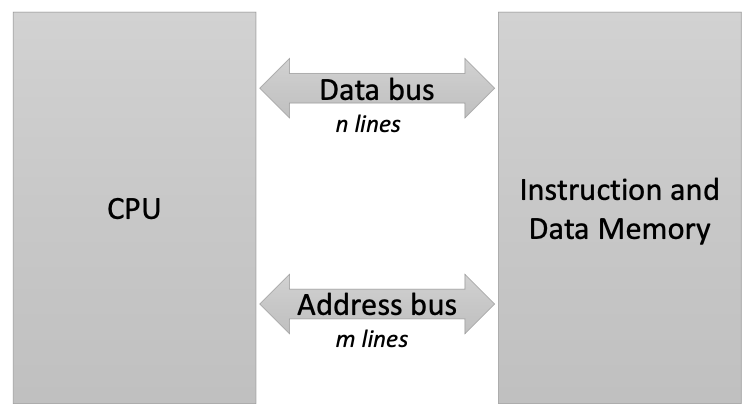
\includegraphics[width=0.5\columnwidth]{img/von_neumann.png}
\end{center}

\subsubsection{Organizzazione di Harward}
\begin{center}
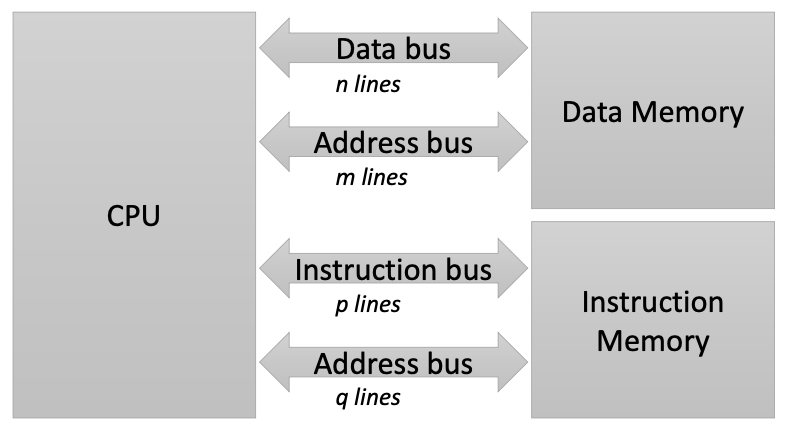
\includegraphics[width=0.5\columnwidth]{img/harward.png}
\end{center}

\subsection{Un'implementazione di base di LEGv8}
Esamineremo un'implementazione che include un sottoinsieme del set di istruzioni di base LEGv8:
Le istruzioni di riferimento della memoria caricano il registro non scalato (LDUR) e memorizzano il registro non scalato (STUR). Le istruzioni aritmetiche-logiche ADD, SUB, AND e ORR. Le istruzioni di confronto e branch se zero (CBZ) e branch (B).\\
Queste operazioni illustrano i principi chiave utilizzati nella creazione di un percorso dati e nella progettazione del controllo. Avremo l'opportunità di vedere: come l'architettura del set di istruzioni determina molti aspetti dell'implementazione e come la scelta delle varie strategie di implementazione influisce sulla frequenza di clock e sul CPI.

\subsection{Esecuzione delle istruzioni}
Molto di ciò che deve essere fatto per implementare queste istruzioni è lo stesso, indipendente dall'esatta classe di istruzione. Per ogni istruzione, i primi due passaggi sono identici:
\begin{enumerate}
\item Invia il progam counter (PC) alla memoria che contiene il codice e recupera l'istruzione da quella memoria.
\item Leggi uno o due registri, usando i campi dell'istruzione per selezionare i registri da leggere.
\end{enumerate}
Dopo questi passaggi, le azioni necessarie per completare l'istruzione dipendono dalla classe di istruzione.\\
A seconda della classe di istruzione\\
\begin{itemize}
\item Usa l'ALU per calcolare
\begin{itemize}
\item Risultato aritmetico
\item Indirizzo di memoria per load/store
\item Confronto con zero nel branch
\end{itemize}
\item Accedi alla memoria dati per il load/store 
\item PC $\leftarrow$ target address o PC + 4
\end{itemize}

\subsection{CPU Overview}
\begin{center}
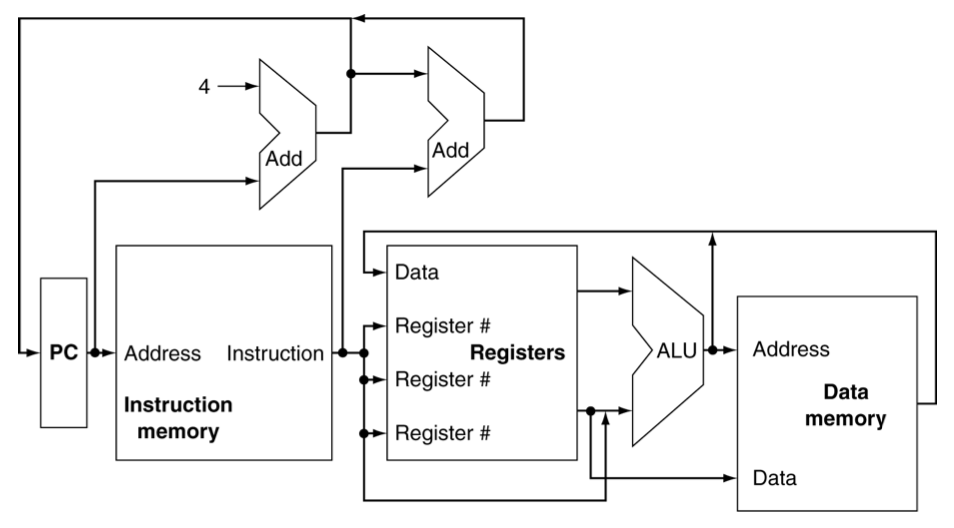
\includegraphics[width=0.5\columnwidth]{img/cpu.png}
\end{center}

\subsubsection{Multiplexer}
\begin{center}
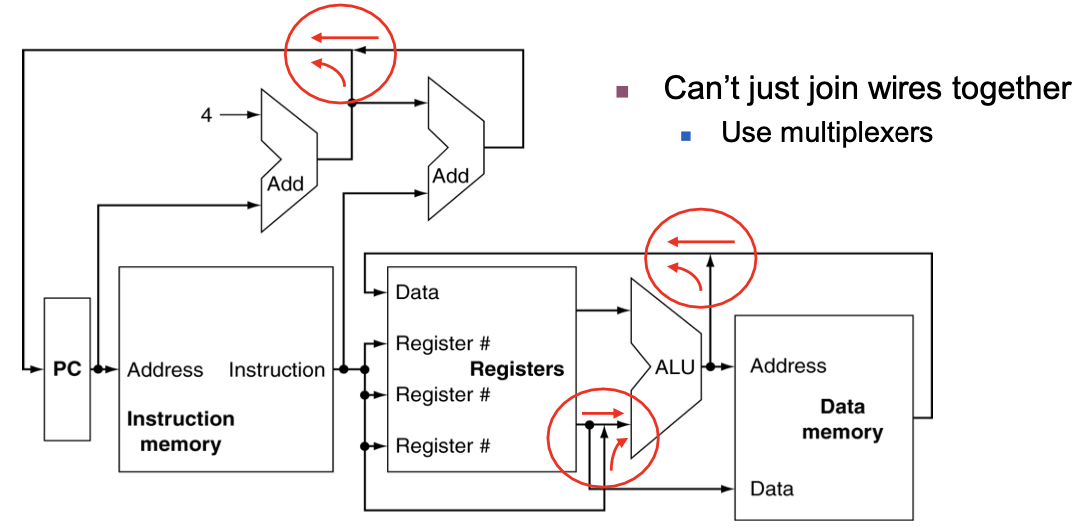
\includegraphics[width=0.5\columnwidth]{img/multiplexer.png}
\end{center}

\subsubsection{Controllore}
\begin{center}
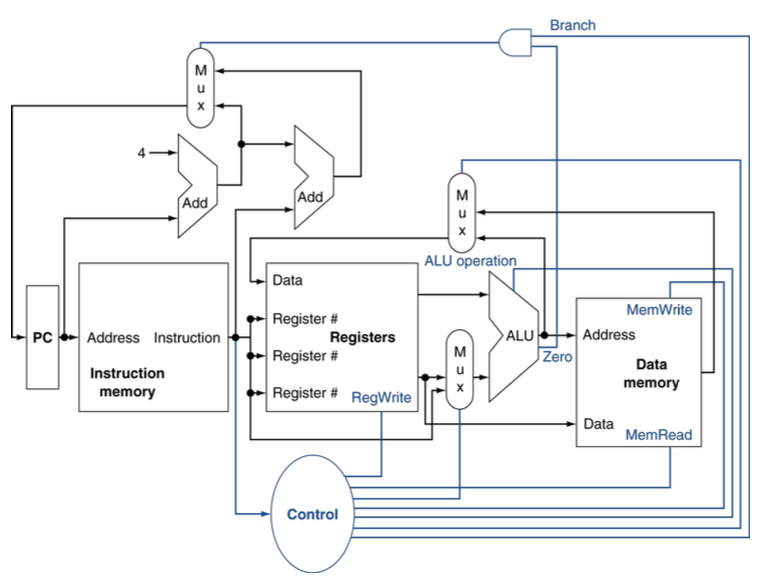
\includegraphics[width=0.5\columnwidth]{img/control.png}
\end{center}

\subsection{Convenzioni di progettazione logica}
Gli elementi del percorso dati nell'implementazione LEGv8 sono costituiti da due diversi tipi di elementi logici:
\begin{itemize}
\item Elementi combinati
\begin{itemize}
\item Operarazioni sui dati
\item L'output è una funzione dell'input
\end{itemize}
\item Elementi di stato (sequenziali)
\begin{itemize}
\item Memorizza informazioni (e.g. registri e memorie)
\item Chiamiamo questi elementi elementi elementi di stato perché, se togliessimo la spina di alimentazione sul computer, potremmo riavviarlo con precisione caricando gli elementi di stato con i valori che contenevano prima di staccare la spina.
\item Un elemento di stato ha almeno due ingressi e un'uscita:
\begin{itemize}
\item Inserimento dati, clock.
\item L'output è il valore che è stato scritto in un ciclo di clock precedente.
\end{itemize}
\end{itemize}
\item Il clock viene utilizzato per determinare quando l'elemento di stato deve essere scritto.
\end{itemize}

\subsection{Metodologia di clocking}
Una metodologia di clock definisce quando i segnali possono essere letti e quando possono essere scritti. Assumeremo una metodologia di clock attivata dall'edge. Tutti i valori memorizzati in un elemento logico sequenziale vengono aggiornati solo sul bordo del clock.
\begin{center}
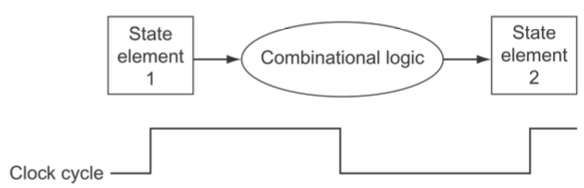
\includegraphics[width=0.5\columnwidth]{img/clocking.png}
\end{center}
Tutti i segnali devono propagarsi dall'elemento di stato 1, attraverso la logica combinata, e allo stato dell'elemento 2 nel tempo di un ciclo di clock. Il tempo necessario affinché i segnali raggiungano l'elemento di stato 2 definisce la lunghezza del ciclo di clock. Se un elemento di stato non viene aggiornato su ogni clock, è necessario un segnale di controllo di scrittura esplicito. L'elemento di stato viene modificato solo quando viene affermato il segnale di controllo e si verifica un bordo del clock.

\subsection{Il percorso dati semplice}
\begin{center}
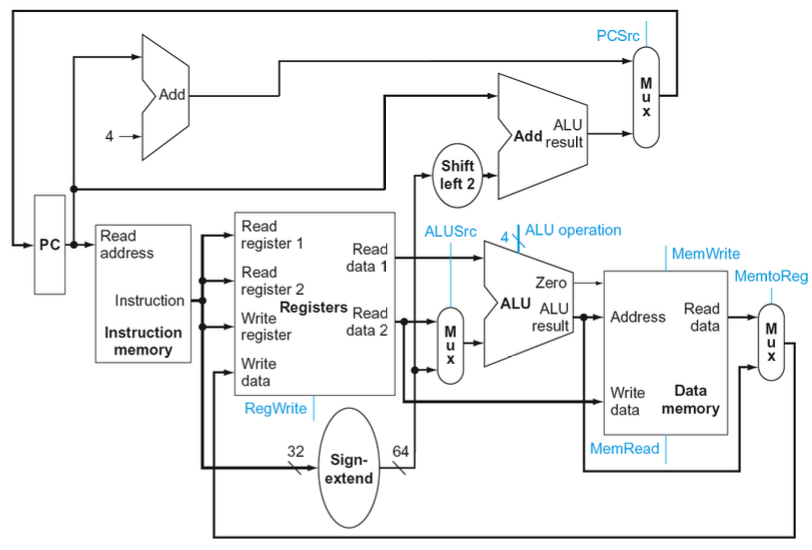
\includegraphics[width=0.7\columnwidth]{img/datapath.png}
\end{center}

\subsubsection{Il percorso dati semplice con controllore}
\begin{center}
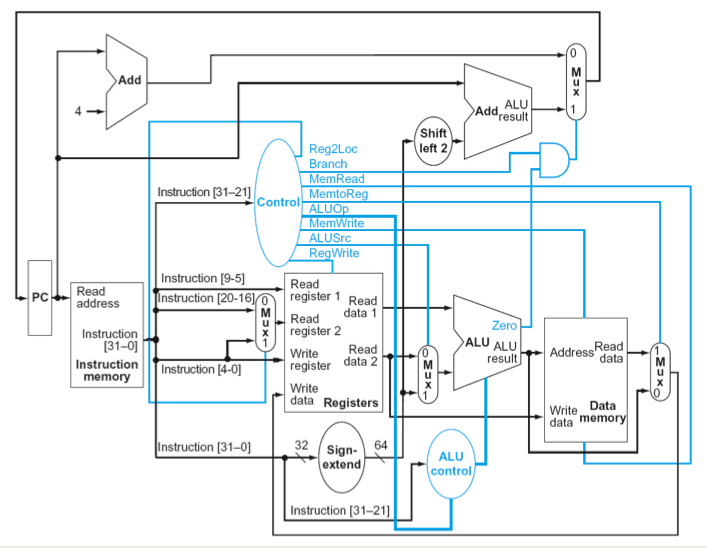
\includegraphics[width=0.7\columnwidth]{img/datapath_control.png}
\end{center}

\subsection{Controllo della ALU}
La ALU viene usata per:
\begin{itemize}
\item Load/Store: Funzione = add
\item Branch: Funzione = compare
\item R-Type: Funzione dipende dall'opcode
\end{itemize}
Assumiamo un ALUOp a 2-bit, dagli opcode sappiamo che:
\begin{itemize}
\item 00 - loads e stores
\item 01 - Passaggio dell'input per il CBZ
\item 10 - determina dall'opcode i campi per le operazioni di tipo R
\end{itemize}

\begin{center}\begin{tabular}{|c|c|}
\hline
\rowcolor[HTML]{FFCB2F} 
ALU Control lines & Funzione \\ \hline
0000 & AND \\ \hline
0001 & OR \\ \hline
0010 & ADD \\ \hline
0110 & SUB \\ \hline
0111 & Input per il branch \\ \hline
1100 & NOR \\ \hline
\end{tabular}

\begin{tabular}{|c|c|c|c|c|c|}
\hline
\rowcolor[HTML]{FFCB2F} 
Tipo & ALUOp & Istruzione & Campi Opcode & Azione ALU & Control input \\ \hline
LDUR & 00 & Load register & XXXXXXX & add & 0010 \\ \hline
STUR & 00 & Store register & XXXXXXX & add & 0010 \\ \hline
CBZ & 01 & CBZ & XXXXXXX & pass input b & 0111 \\ \hline
Tipo R & 10 & ADD & 10001011000 & addizione & 0010 \\ \hline
Tipo R & 10 & SUB & 11001011000 & sottrazione & 0110 \\ \hline
Tipo R & 10 & AND & 10001010000 & AND & 0000 \\ \hline
Tipo R & 10 & ORR & 10101010000 & OR & 0001 \\ \hline
\end{tabular}\end{center}

\subsection{Formato istruzioni}
Vedremo l'implementazione di queste 3 istruzioni:
\begin{verbatim}
ADD X1, X2, X3
LDUR X1, [X2, offset]
CBZ X1, offset
\end{verbatim}
\begin{tabular}{ll}
\begin{tabular}{l}
Campo\\
Posizione bit\\
Istruzione di tipo R\\
\end{tabular} & \begin{tabular}{cccccc}
\hline
\multicolumn{2}{|c|}{opcode} & \multicolumn{1}{c|}{Rm} & \multicolumn{1}{c|}{shamt} & \multicolumn{1}{c|}{Rn} & \multicolumn{1}{c|}{Rd} \\ \hline
\multicolumn{2}{c}{31:21} & 20:16 & 15:10 & 9:5 & 4:0 \\
 &  &  &  &  & 
\end{tabular}\\
\begin{tabular}{l}
Campo\\
Posizione bit\\
Istruzione di load/store\\
\end{tabular} & \begin{tabular}{clcccc}
\hline
\multicolumn{2}{|c|}{1986 o 1984} & \multicolumn{1}{c|}{indirizzo} & \multicolumn{1}{c|}{0} & \multicolumn{1}{c|}{Rn} & \multicolumn{1}{c|}{Rt} \\ \hline
\multicolumn{2}{c}{31:21} & 20:12 & 11:10 & 9:5 & 4:0\\
& & & & & 
\end{tabular}\\
\begin{tabular}{l}
Campo\\
Posizione bit\\
Istruzione di Conditional branch\\
\end{tabular} & \begin{tabular}{cccccc}
\hline
\multicolumn{2}{|c|}{180} & \multicolumn{3}{c|}{indirizzo} & \multicolumn{1}{c|}{Rt} \\ \hline
\multicolumn{2}{c}{31:24} & \multicolumn{3}{c}{23:5} & 4:0 \\
 &  &  &  &  & 
\end{tabular}
\end{tabular}\\
Ci sono diverse osservazioni importanti su questo formato di istruzioni su cui faremo affidamento:
\begin{itemize}
\item Il campo opcode è largo tra 6 e 11 bit e si trova nei bit da 31:26 a 31:21.
\item Il primo operando del registro è sempre in posizioni di bit 9:5 (Rn) sia per le istruzioni di tipo R che per il registro di base per le istruzioni di carico e conservazione.
\item L'altro registro operando si trova in uno dei due posti. È in posizioni di bit 20:16 (Rm) per istruzioni di tipo R ed è in posizioni di bit 4:0 (Rt) che il registro sia scritto da un load. Anche questo è il campo che specifica il registro da testare per zero per confrontare e saltare se zero.
\item Un altro operando può anche essere un offset a 19 bit per confrontare e saltare se zero o un offset a 9 bit per load e store.
\item Il registro di destinazione per le istruzioni di tipo R (Rd) e per i load (Rt) è in posizioni di bit 4:0.
\end{itemize}

\subsubsection{ADD X1, X2, X3}
Anche se tutto avviene in un ciclo di clock, possiamo pensare a quattro passaggi per eseguire l'istruzione, questi passaggi sono ordinati dal flusso di informazioni:
\begin{enumerate}
\item L'istruzione viene recuperata e il PC viene incrementato.
\item Due registri, X2 e X3, vengono letti dal file del registro; inoltre, l'unità di controllo principale calcola l'impostazione delle linee di controllo durante questo passaggio.
\item L'ALU opera sui dati letti dal file di registro, utilizzando parti dell'opcode per generare la funzione ALU.
\item Il risultato dell'ALU è scritto nel registro di destinazione (X1) nel file del registro.
\end{enumerate}
\begin{center}
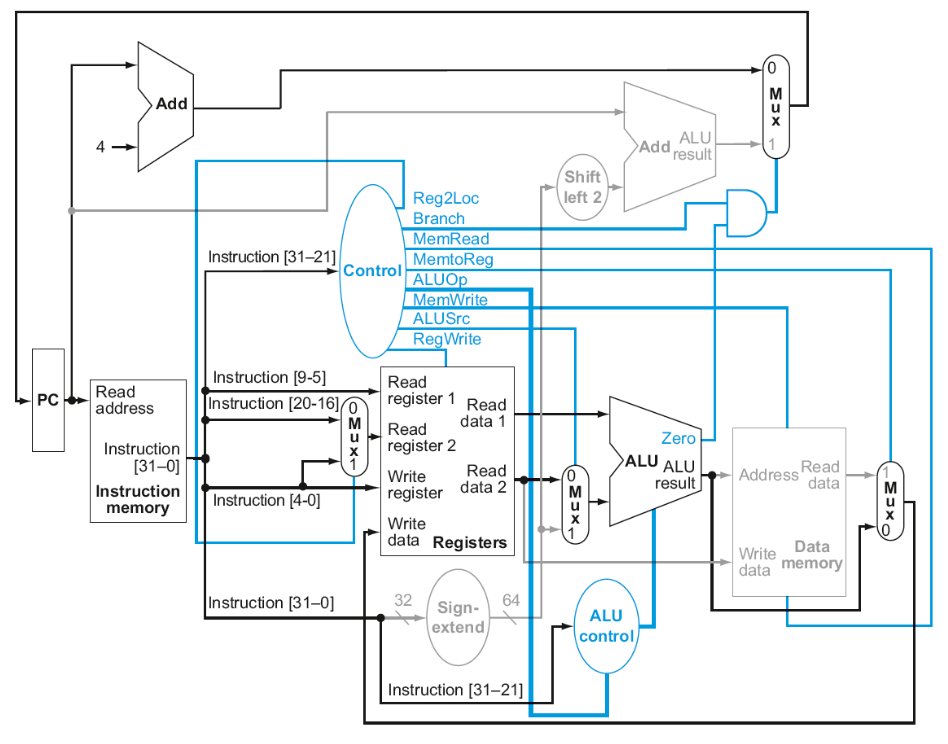
\includegraphics[width=0.6\columnwidth]{img/add_x1x2x3.png}
\end{center}

\subsubsection{LDUR X1, [X2, offset]}
Possiamo pensare a un'istruzione di carico come operativa in cinque passaggi:
\begin{enumerate}
\item Un'istruzione viene recuperata dalla memoria dell'istruzione e il PC viene incrementato.
\item Un valore di registro (X2) viene letto dal file del registro.
\item L'ALU calcola la somma del valore letto dal file del registro e i 9 bit estesi dal segno dell'istruzione (offset).
\item La somma dell'ALU viene utilizzata come indirizzo per la memoria dati.
\item I dati dell'unità di memoria vengono scritti nel file di registro (X1).
\end{enumerate}
\begin{center}
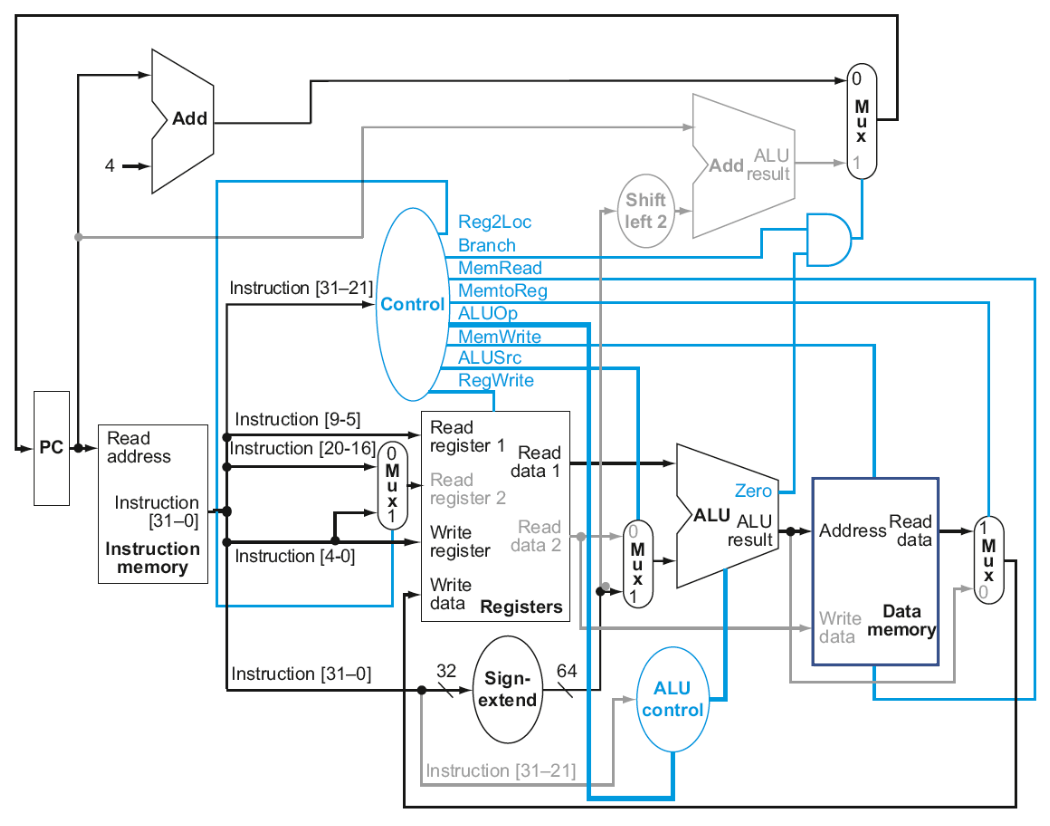
\includegraphics[width=0.6\columnwidth]{img/ldur_x1x2.png}
\end{center}

\subsubsection{CBZ X1, offset}
Funziona in modo molto simile a un'istruzione in formato R, ma l'output ALU viene utilizzato per determinare se il PC è scritto con PC + 4 o l'indirizzo di destinazione del ramo.\\
Possiamo pensare a quattro passaggi nell'esecuzione:
\begin{enumerate}
\item Un'istruzione viene recuperata dalla memoria dell'istruzione e il PC viene incrementato.
\item Il registro X1 viene letto dal file del registro usando i bit 4:0 dell'istruzione (Rt).
\item L'ALU passa il valore dei dati letto dal file del registro. Il valore del PC viene aggiunto al segno-esteso, 19 bit dell'istruzione (offset) vengono spostati a sinistra di due; il risultato è il ramo indirizzo target.
\item Le informazioni sullo stato zero dell'ALU vengono utilizzate per decidere quale risultato memorizzare nel PC.
\end{enumerate}
\begin{center}
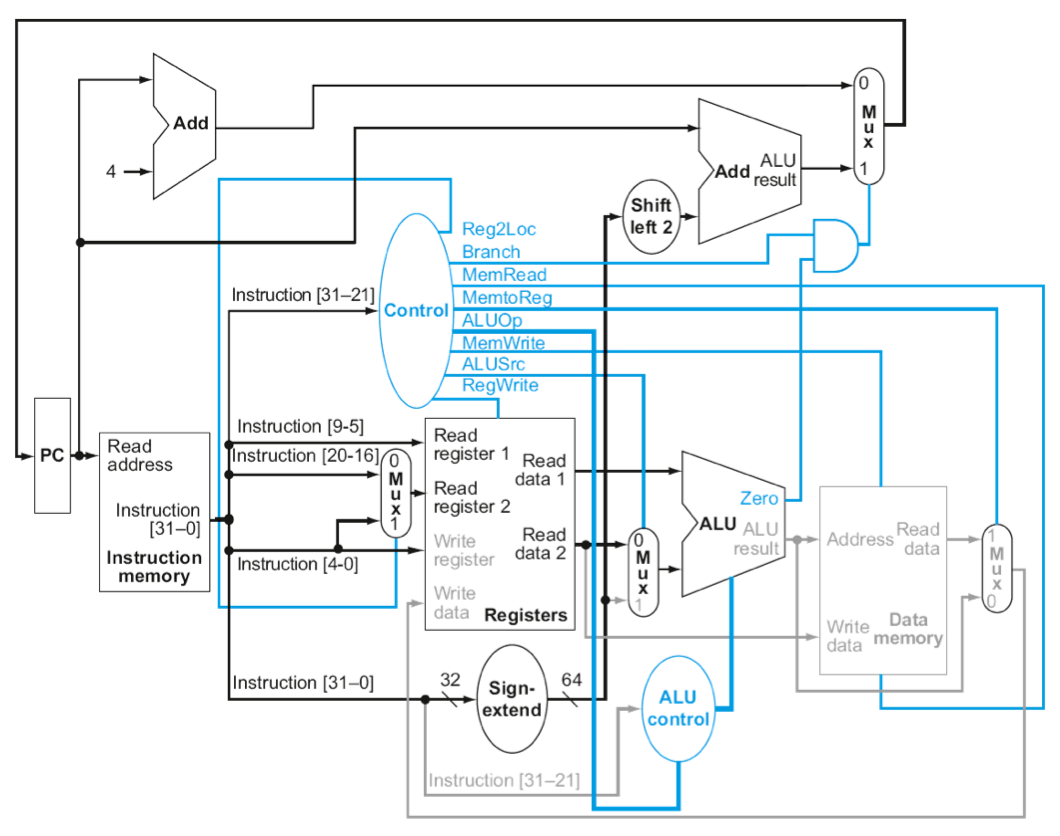
\includegraphics[width=0.6\columnwidth]{img/cbz_x1.png}
\end{center}

\subsection{Perché un'implementazione a ciclo singolo non viene utilizzata oggi?}
Anche se il design a ciclo singolo funzionerà correttamente, è troppo inefficiente per essere utilizzato nei design moderni. Si noti che il ciclo di clock deve avere la stessa lunghezza per ogni istruzione in questo progetto a ciclo singolo. Il percorso più lungo possibile nel processore determina il ciclo di clock; questo percorso è molto probabilmente un'istruzione di load, che utilizza cinque unità funzionali in serie: la memoria di istruzioni, il file di registro, l'ALU, la memoria dati e il file di registro.
Sebbene il CPI sia 1, è probabile che le prestazioni complessive di un'implementazione a ciclo singolo siano scarse, dal momento che il ciclo di clock è troppo lungo. Storicamente, i primi computer con set di istruzioni molto semplici utilizzavano questa tecnica di implementazione. Tuttavia, se provassimo ad implementare l'unità in virgola mobile o un set di istruzioni con istruzioni più complesse, questo design a ciclo singolo non funzionerebbe affatto bene.

\subsection{Strategie di controllo multiciclo}
\begin{center}
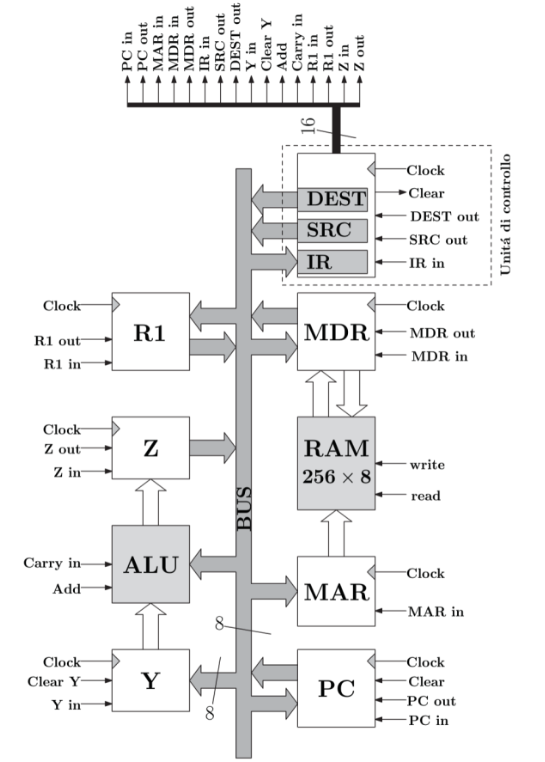
\includegraphics[width=0.5\columnwidth]{img/multiciclo.png}
\end{center}
Consideriamo l'ipotetico processore della figura. L'unità di controllo decodifica ed esegue le istruzioni e aggiorna il contatore del programma (PC), recuperando la prossima istruzione. L'unità di controllo è qui composta da tre registri:
\begin{itemize}
\item IR ha l'OpCode dell'istruzione
\item SRC può contenere un parametro incluso nell'IW o un indirizzo di memoria, spesso espresso in termini relativi come incremento del PC.
\item DEST può contenere un indirizzo o il puntatore a un registro dove scrivere il risultato.
\end{itemize}
Dall'analisi dell'OpCode, l'unità di controllo deve fornire la sequenza di segnali di controllo necessari per
\begin{enumerate}
\item Recupera e aggiorna il PC
\item Esecuzione dell'istruzione attuale
\end{enumerate}
Storicamente, sono stati seguiti due possibili approcci per l'unità di controllo:
\begin{itemize}
\item Approccio microprogrammato
\item Approccio cablato
\item I microcontrollori con vecchie architetture sono microprogrammati. Quelli più recenti, in particolare quelli RISC, sono cabati.
\end{itemize}
Due possibili strategie di clocking:
\begin{itemize}
\item Controllo multiciclo: Recupera, decodifica, esegui eseguito con più periodi di clock.
\item Controllo a ciclo singolo: Recupera, decodifica, esegui eseguito in un unico periodo.
\end{itemize}
 La strategia di controllo a ciclo singolo viene impiegata solo nei controlli cablati.\\
 La strategia di controllo multiciclo viene utilizzata sia in tutti i controlli microprogrammati che in alcuni controlli cablati.

\subsection{Controllori microprogrammati}
È implementato con un'unità di controllo che replica la struttura di una semplice CPU con una memoria, un PC, un ALU, chiamato motore di microcodici. Ogni macro-istruzione corrisponde a un microcodice, composto da alcune parole. I microcodici sono memorizzati in una memoria ROM.\\
Due possibilità:
\begin{itemize}
\item Microprogrammazione orizzontale: l'unità di controllo esegue il codice rigorosamente in sequenza, avviando dall'indirizzo indicato dall'OpCode.
\item Microprogrammazione verticale: sono possibili salti e consentono di ripetere segmenti di microcodice, cioè l'introduzione di micro-subroutine.
\end{itemize}
Il microcodice è composto da parole, i cui bit affermano/negano direttamente segnali di controllo specifici. La lunghezza delle parole del microcodice dipende dal numero di segnali di controllo.
\begin{center}
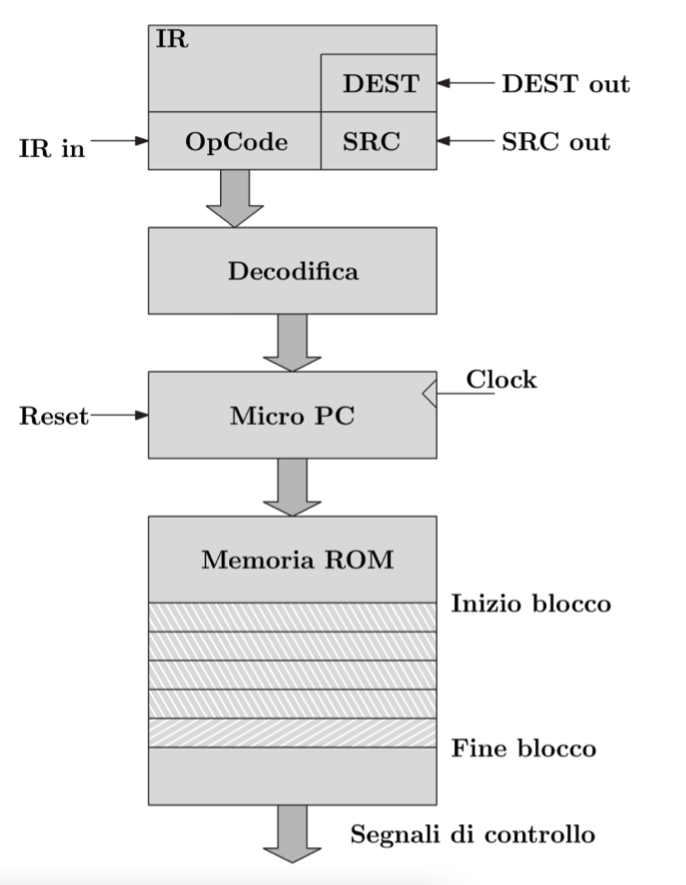
\includegraphics[width=0.5\columnwidth]{img/microprogrammed.png}
\end{center}

\subsection{Controllore cablato}
Il motore di microcodice viene sostituito da un circuito logico combinatorio che genera direttamente i segnali di controllo dall'OpCode dell'istruzione corrente, gestendo anche le temporizzazioni. Include un generatore di clock secondario, il cui scopo è la distribuzione temporale delle attivazioni del segnale di controllo.\\
Supponiamo che una singola istruzione venga eseguita in 7 periodi. Il generatore di clock secondario è un divisore di clock per 7 che genera 1 impulso ogni 7 periodi di clock, e alimenta un registro dei turni di 6 FlipFlops. Il decodificatore attiva una linea di uscita per ogni OpCode. La rete combinatoria, composta da porte AND e OR, alimenta le linee di controllo sulla base dell'OpCode e lo stato di clock secondario (da 1 a 7).\\
La soluzione fornisce una risposta molto rapida, con poca occupazione nell'area del silicio, ma manca di flessibilità, e potrebbe essere necessario cicli nop per gestire istruzioni più brevi.
\begin{center}
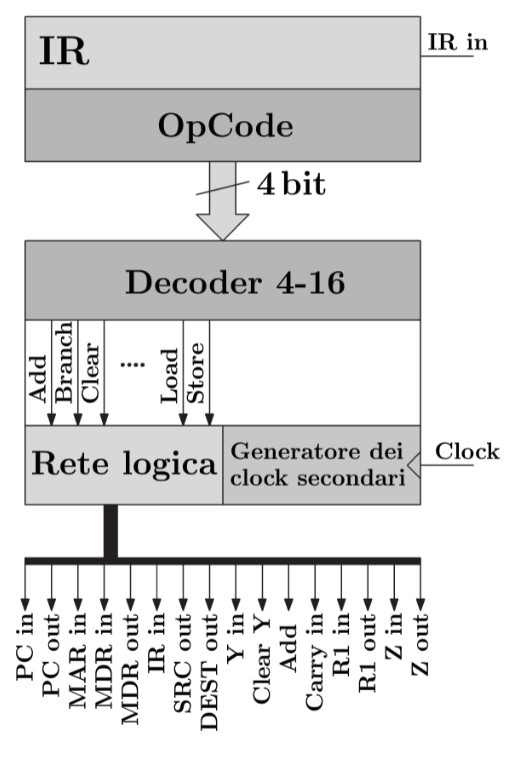
\includegraphics[width=0.4\columnwidth]{img/cabled.png}
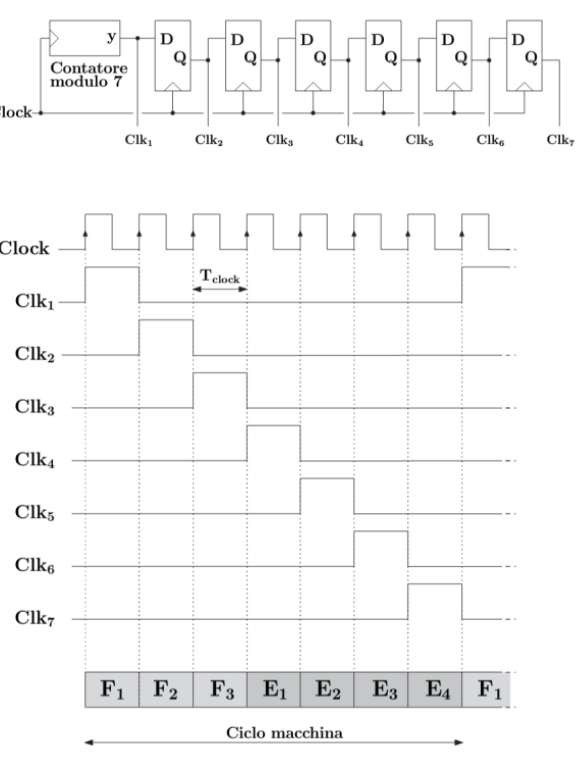
\includegraphics[width=0.4\columnwidth]{img/cabled_2.png}
\end{center}

\subsection{Organizzazione Multi ciclo vs Singolo ciclo}
Solo la disponibilità di più risorse consente una temporizzazione a ciclo singolo. Richiede almeno che la fase di recupero venga eseguita contemporaneamente per decodificare ed eseguire. Impone i seguenti requisiti di sistema:
\begin{itemize}
\item Memoria dati separata e memoria di istruzioni
\item ALU separata per l'incremento del PC
\item Incremento flessibile del PC per la gestione dei salti senza l'intervento principale di ALU
\end{itemize}
A meno che il set di istruzioni non sia molto semplice, l'organizzazione a ciclo singolo è spesso inefficiente. \'E l'istruzione più onerosa che determina il periodo di clock. Al contrario, nell'organizzazione multiciclo, è l'unità funzionale più lenta (ALU o memoria) che determina il periodo minimo. \'E possibile combinare i vantaggi di entrambi, utilizzando un'organizzazione di pipeline.

\subsection{Pipeline}
La pipeline è una tecnica di implementazione in cui più istruzioni sono sovrapposte nell'esecuzione. Oggi, la pipelining è quasi universale.\\
\textbf{Facciamo una piccola analogia}: Esecuzione sovrapposta del bucato. Il parallelismo migliora le prestazioni
\begin{center}
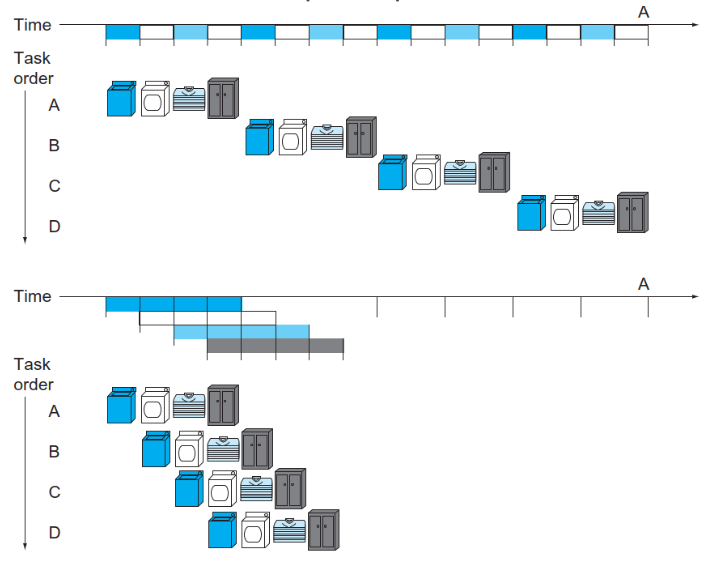
\includegraphics[width=0.6\columnwidth]{img/pipeline.png}
\end{center}
In questo caso abbiamo:
\begin{itemize}
\item 4 Carichi $\rightarrow$ Accelerazione $= {16 \over 7} = 2.3$
\item Non-stop $\rightarrow$ Accelerazione $={4n \over 1n + 3} \simeq 4 =$ numero di fasi
\end{itemize}
Il paradosso della pipelining è che il tempo per l'elaborazione di un singolo carico di lavanderia non è più breve per il pipelining.
Ma più carichi vengono elaborati all'ora. La pipeline migliora la produttività del nostro sistema di lavanderia.

\subsubsection{Prestazioni a Singolo ciclo vs Pipeline}
Le istruzioni LEGv8 classicamente fanno cinque passaggi:
\begin{enumerate}
\item Recupera le istruzioni a memoria.
\item Leggi i registri e decodifica le istruzioni.
\item Esegui l'operazione o calcola un indirizzo.
\item Accedi a un operando nella memoria dati (se necessario).
\item Scrivi il risultato in un registro (se necessario).
\end{enumerate}
Quindi, la pipeline del LEGv8 che consideriamo ha cinque fasi.\\
Limitiamo la nostra attenzione a sette istruzioni: registro di carico (LDUR), registro del negozio (STUR), aggiunta (ADD), sottrazione (SUB), AND (AND), OR (ORR) e confronto e diramazione a zero (CBZ). Supponiamo che il tempo per le fasi sia 100ps per la lettura o la scrittura del registro 200ps per altre fasi.
\begin{center}
\resizebox{\textwidth}{!}{%
\begin{tabular}{|l|c|c|c|c|c|c|}
\hline
\rowcolor[HTML]{FFCB2F} 
\multicolumn{1}{|c|}{\cellcolor[HTML]{FFCB2F}Classe di istruzioni} & Fetch & Lettura registro & Operazione ALU & Accesso dati & Scrittura registro & Tempo Totale \\ \hline
Load (LDUR) & 200 ps & 100 ps & 200 ps & 200 ps & 100 ps & 800 ps \\ \hline
Store (STUR) & 200 ps & 100 ps & 200 ps & 200 ps &  & 700 ps \\ \hline
Formato R (ADD, SUB, AND, ORR) & 200 ps & 100 ps & 200 ps &  & 100 ps & 600 ps \\ \hline
Branch (CBZ) & 200 ps & 100 ps & 200 ps &  &  & 500 ps \\ \hline
\end{tabular}}\end{center}
\begin{center}
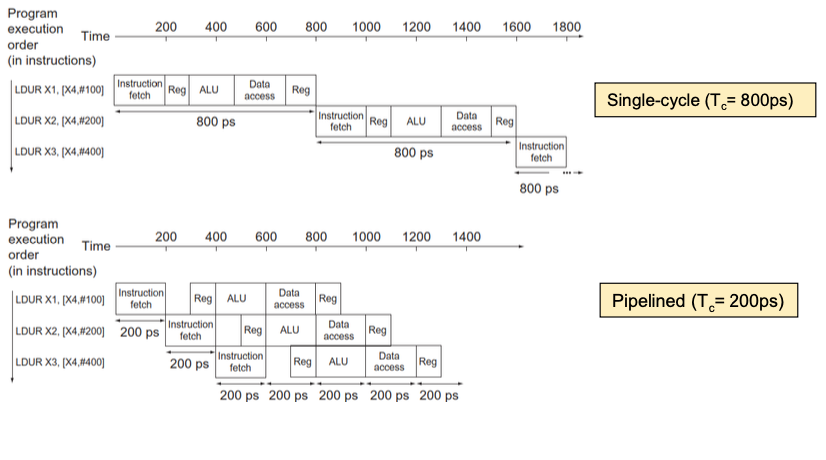
\includegraphics[width=0.6\columnwidth]{img/single_vs_pipeline.png}
\end{center}

\subsection{Accelerazione della Pipeline}
Se le fasi sono perfettamente bilanciate, allora
$$Tempo\ tra\ le\ istruzioni_{pipeline} = {Tempo\ tra\ le\ istruzioni_{Non\ pipeline} \over Numero\ di\ fasi\ della\ pipeline}$$
In condizioni ideali e con un gran numero di istruzioni, l'accelerazione della pipeline è approssimativamente uguale al numero di stadi di pipeline. Se le fasi non sono bilanciate, la velocità è inferiore. Inoltre, vedremo che la pipeline comporta un po' di spese generali.\\
In realtà, nel nostro caso il tempo di esecuzione totale per le tre istruzioni è di 1400 ps contro 2400 ps. Ma se aggiungiamo 1.000.000 di istruzioni: ${800.002.400\ ps \over 200.001.400\ ps} \simeq {800 \over 200} \simeq 4$
La pipeline migliora le prestazioni aumentando la produttività delle istruzioni, in contrasto con la diminuzione del tempo di esecuzione di una singola istruzione.

\subsection{Progettazione di set di istruzioni per la pipeline}
LEGv8 è stato progettato per l'esecuzione in pipeline:
\begin{itemize}
\item Tutte le istruzioni sono a 32 bit: Più facile da recuperare e decodificare in un ciclo, c.f. x86: istruzioni da 1 a 17 byte
\item Pochi e regolari formati di istruzioni: Può decodificare e leggere i registri in un unico passaggio
\item Gli operandi di memoria appaiono solo nei carichi o nei negozi: Possiamo usare la fase di esecuzione per calcolare l'indirizzo di memoria e quindi accedere alla memoria nella fase successiva.
\end{itemize}

\subsubsection{Pericoli della pipeline}
Ci sono situazioni nel pipelining in cui l'istruzione successiva non può essere eseguita nel seguente ciclo di clock. Questi eventi sono chiamati pericoli e ce ne sono tre diversi tipi:
\begin{itemize}
\item \textbf{Pericoli di struttura}: Quando un'istruzione pianificata non può essere eseguita nel ciclo di clock corretto perché l'hardware non supporta la combinazione di istruzioni impostate per l'esecuzione.
\item \textbf{Pericolo di dati}: Quando un'istruzione pianificata non può essere eseguita nel ciclo di clock corretto perché i dati che sono necessario per eseguire le istruzioni non sono ancora disponibili.
\item \textbf{Pericolo di controllo} (chiamato anche pericolo di branch): Quando l'istruzione corretta non può essere eseguita nel ciclo di clock della pipeline corretto perché l'istruzione che è stata recuperata non è quella necessaria; cioè, il flusso degli indirizzi di istruzioni non è quello che la pipeline si aspettava.
\end{itemize}

\subsubsection{Pericoli strutturali}
Quando un'istruzione pianificata non può essere eseguita nel ciclo di clock corretto perché l'hardware non supporta la combinazione di istruzioni impostate per l'esecuzione. Il set di istruzioni LEGv8 è stato progettato per essere utilizzato in pipeline, rendendo abbastanza facile per i progettisti evitare rischi strutturali durante la progettazione di una pipeline.\\
Supponiamo, tuttavia, di avere una sola memoria invece di due:
\begin{itemize}
\item Il load/store richiede l'accesso ai dati
\item Il recupero delle istruzioni dovrebbe bloccarsi per quel ciclo (creerebbe una "bolla" della pipeline)
\end{itemize}
Quindi, i percorsi dati della pipeline richiedono istruzioni/memorie di dati separate (O cache di istruzioni/dati separate)
\subsubsection{Pericoli di dati}
I rischi di dati derivano dalla dipendenza di un'istruzione da una precedente che è ancora in lavorazione.\\
Ad esempio:
\begin{center}
\begin{minipage}{.2\linewidth}
\begin{verbatim}
ADD X19, X0, X1
SUB X2, X19, X3
\end{verbatim}
\end{minipage}
\end{center}
\begin{center}
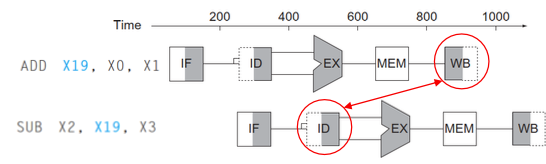
\includegraphics[width=0.6\columnwidth]{img/data_hazard.png}
\end{center}

\paragraph{Pericolo di dati per l'uso del Load}
L'inoltro non può impedire lo stallo all'interno della pipeline. Supponiamo che la prima istruzione sia stata un carico di X1 invece di un'aggiunta. I dati desiderati sarebbero disponibili solo dopo la quarta fase della prima istruzione nella dipendenza, che è troppo tardi per l'ingresso del terzo stadio di SUB.
\begin{center}
\includegraphics[width=0.6\columnwidth]{img/load-use.png}
\end{center}
Il pericolo di dati per l'uso del load è una forma specifica di pericolo di dati in cui i dati caricati da un'istruzione di carico non sono ancora diventati disponibili quando sono necessari da un'altra istruzione.
Lo \textbf{stallo della pipeline} viene chiamato anche \textbf{bolla}. Uno stallo viene avviato per risolvere un pericolo.
\paragraph{Riordinare il codice per evitare stalli della pipeline} Possiamo prevenire il pericolo di utilizzo dei dati di carico riordinando il codice per evitare l'uso del risultato del carico nelle istruzioni successive.\\
Codice C per
\begin{center}
\begin{minipage}{.2\linewidth}
\begin{verbatim}
A = B + E;
C = B + F;
\end{verbatim}
\end{minipage}
\end{center}
\begin{center}
\includegraphics[width=0.6\columnwidth]{img/stall_reorder.png}
\end{center}

\subsubsection{Pericoli di controllo}
Pericolo di controllo chiamato anche pericolo di branch. Quando l'istruzione corretta non può essere eseguita nel corretto ciclo di clock della pipeline perché l'istruzione che è stata recuperata non è quella necessaria; cioè, il flusso degli indirizzi di istruzioni non è ciò che la pipeline si aspettava.\\
Nell'istruzione del branch condizionale, dobbiamo iniziare a recuperare l'istruzione seguendo il branch nel seguente ciclo di clock. Tuttavia, la pipeline non può assolutamente sapere quale dovrebbe essere la prossima istruzione, dal momento che ha appena ricevuto l'istruzione del branch dalla memoria!\\
Nella pipeline LEGv8:
\begin{itemize}
\item Dobbiamo confrontare i registri e calcolare l'obiettivo all'inizio della pipeline.
\item Supponiamo di aver inserito abbastanza hardware extra in modo da poter testare un registro, calcolare l'indirizzo della filiale e aggiornare il PC durante la seconda fase della pipeline (fase ID).
\end{itemize}

\paragraph{Stallo sui Branch}
Una possibile soluzione è quella di bloccarsi immediatamente dopo aver recuperato il branch, aspettando che la pipeline determini l'esito del branch.
\begin{center}
\includegraphics[width=0.6\columnwidth]{img/stall_branch.png}
\end{center}
\textbf{Performance}: Stimare l'impatto sui cicli di clock per istruzione (CPI) dello stallo sui branch. Supponiamo che tutte le altre istruzioni abbiano un CPI di 1.\\
I branch condizionali rappresentano il 17\% delle istruzioni eseguite in SPECint2006. Poiché le altre istruzioni (83\%) hanno un CPI di 1 e i branch condizionali hanno preso un ciclo di clock in più per lo stallo, quindi vedremo un CPI di
$$CPI:0.83*1+0.17*2=1.17$$
Quindi un rallentamento di 1,17 rispetto al caso ideale.

\paragraph{Predizione dei branch}
Se non riusciamo a risolvere il branch nella seconda fase, come spesso accade per le pipeline più lunghe, allora vedremmo un rallentamento ancora più grande che se ci bloccassimo sui branch condizionali. Il costo di questa opzione è troppo alto per la maggior parte dei computer da utilizzare e motiva una seconda soluzione al rischio di controllo: prevedere l'esito del ramo.\\
Questa opzione non rallenta la pipeline quando prevede correttamente.\\
Quando sbagli: devi rifare il load che non è stato fatto mentre si cercava di prevedere la decisione (con la creazione di una bolla).\\
Un semplice approccio è prevedere sempre che i branch condizionali non saranno affrontati. Quando hai ragione, la pipeline procede a tutta velocità. Solo quando vengono prelevati rami condizionali, la pipeline si blocca.
\begin{center}
\includegraphics[width=0.6\columnwidth]{img/branch_prediction.png}
\end{center}

\paragraph{Predizione dei branch più realistica}
Una versione più sofisticata della previsione dei branch avrebbe alcuni branch condizionali previsti come presi e alcuni come non presi.
\begin{itemize}
\item \textbf{Previsione del branch statico}:
\begin{itemize}
\item Basato sul tipico comportamento del branch
\item Esempio: branch loop e if-statement: Prevedi i branch presi in precedenza, prevedi i branch in avanti non presi\end{itemize}
\item \textbf{Previsione dinamica dei branch}
\begin{itemize}
\item L'hardware misura il comportamento effettivo del branch. Ad esempio, registrare la storia recente di ciascun branch
\item Supponiamo che il comportamento futuro continui la tendenza. Quando sbaglio, fermati durante il recupero e aggiorna la cronologia
\end{itemize}\end{itemize}

\paragraph{Terzo approccio: branch ritardato}
C'è un terzo approccio al pericolo di controllo, chiamato branch ritardato. Utilizzato in MIPS, TI C54 e molti altri processori.\\
Il branch ritardato esegue sempre l'istruzione sequenziale successiva, con il branch che si svolge dopo quel ritardo nell'istruzione. \'E nascosto al programmatore del linguaggio assembly MIPS perché l'assembler può organizzare automaticamente le istruzioni per ottenere il comportamento del branch desiderato dal programmatore.\\
Il software MIPS inserirà un'istruzione immediatamente dopo l'istruzione del branch ritardata che non è influenzata dal branch.\\ Un branch preso cambia l'indirizzo dell'istruzione che segue l'istruzione sicura.

\subsubsection{Riepilogo della pipeline: il quadro generale}
La pipeline aumenta il numero di istruzioni di esecuzione simultanea e la velocità con cui le istruzioni vengono avviate e completate.\\
La pipeline non riduce il tempo necessario per completare un'istruzione individuale, cioè la latenza. Ad esempio, la pipeline a cinque stadi richiede ancora cinque cicli di clock per completare l'istruzione.\\
La pipeline migliora il throughput delle istruzioni piuttosto che il tempo di esecuzione delle singole istruzioni.\\
I set di istruzioni possono rendere la vita più difficile o più semplice per i progettisti di pipeline, che devono già far fronte con rischi strutturali, di controllo e di dati.\\
La previsione e l'inoltro dei branch aiutano a rendere veloce un computer pur ottenendo le risposte giuste.

\subsection{Pipeline Datapath in LEGv8}
\begin{center}
\includegraphics[width=0.6\columnwidth]{img/pipeline_legv8.png}
\end{center}

\subsubsection{Registri di pipeline}
Ha bisogno di registri tra le fasi per contenere le informazioni prodotte nel ciclo precedente
\begin{center}
\includegraphics[width=0.6\columnwidth]{img/pipeline_legv8.png}
\end{center}

\subsubsection{Operazioni della pipeline}
Flusso ciclo per ciclo di istruzioni attraverso il percorso dati in pipeline
\begin{itemize}
\item Diagramma della pipeline "A ciclo singolo"
\begin{itemize}
\item Mostra l'utilizzo della pipeline in un unico ciclo
\item Evidenzia le risorse utilizzate
\end{itemize}
\item c.f. diagramma “ciclo multi-clock”\\
Grafico del funzionamento nel tempo
\end{itemize}

\subsubsection{IF per Load, Store, \dots}
\begin{center}
\includegraphics[width=0.6\columnwidth]{img/pipeline_if.png}
\end{center}

\subsubsection{ID per Load, Store, \dots}
\begin{center}
\includegraphics[width=0.6\columnwidth]{img/pipeline_id.png}
\end{center}

\subsubsection{EX per Load}
\begin{center}
\includegraphics[width=0.6\columnwidth]{img/pipeline_ex.png}
\end{center}

\subsubsection{MEM per Load}
\begin{center}
\includegraphics[width=0.6\columnwidth]{img/pipeline_mem.png}
\end{center}

\subsubsection{WB per Load}
\begin{center}
\includegraphics[width=0.6\columnwidth]{img/pipeline_wb.png}
\end{center}
\begin{center}
\includegraphics[width=0.6\columnwidth]{img/pipeline_wb_bis.png}
\end{center}

\subsubsection{Datapath corretto per il Load}
\begin{center}
\includegraphics[width=0.6\columnwidth]{img/load_correct.png}
\end{center}

\subsubsection{EX per Store}
\begin{center}
\includegraphics[width=0.6\columnwidth]{img/pipeline_ex_store.png}
\end{center}

\subsubsection{MEM per Store}
\begin{center}
\includegraphics[width=0.6\columnwidth]{img/pipeline_mem_store.png}
\end{center}

\subsubsection{WB per Store}
\begin{center}
\includegraphics[width=0.6\columnwidth]{img/pipeline_wb_store.png}
\end{center}

\subsection{Diagramma della pipeline Multi ciclo}
\begin{center}
\includegraphics[width=0.6\columnwidth]{img/pipeline_multiciclo.png}
\end{center}
Forma tradiazionale:
\begin{center}
\includegraphics[width=0.6\columnwidth]{img/pipeline_multiciclo_trad.png}
\end{center}

\subsection{Diagramma della pipeline a Singolo ciclo}
Stato della pipeline in un dato ciclo:
\begin{center}
\includegraphics[width=0.6\columnwidth]{img/pipeline_singolociclo.png}
\end{center}

\subsection{Controllo pipeline (semplificato)}
\begin{center}
\includegraphics[width=0.6\columnwidth]{img/pipeline_control_simp.png}
\end{center}

\subsubsection{Controllo pipeline}
Segnali di controllo derivati dall'istruzione. Come nell'implementazione a ciclo singolo
\begin{center}
\includegraphics[width=0.6\columnwidth]{img/pipeline_control_1.png}
\end{center}

\subsection{Pericoli di dati nelle istruzioni ALU}
Consideriamo la sequenza:
\begin{verbatim}
SUB X2, X1, X3 // X2 scritto da SUB
AND X12, X2, X5 // Il primo operando (X2) dipende dal SUB
OR X13, X6, X2 // Il secondo operando (X2) dipende dal SUB 
ADD X14, X2, X2 // Entrambi gli operandi dipendono dal SUB
STUR X15, [X2, #100] // La Base dipende dal SUB
\end{verbatim}
Possiamo risolvere i pericoli con il forwarding. Come rileviamo quando fare il forward?
\subsubsection{Dipendenze \& Forwarding}
\begin{center}
\includegraphics[width=0.6\columnwidth]{img/pipeline_forwarding.png}
\end{center}

\subsubsection{Rilevare la necessità di forward}
Passa i numeri del registro lungo la pipeline. Ad esempio, ID/EX.RegisterRs = numero di registro per Rs situato nel registro della pipeline ID/EX\\
I numeri di registro degli operandi ALU nella fase EX sono forniti da ID/EX.RegisterRn1, ID/EX.RegisterRm2\\
Pericoli di dati quando
\begin{enumerate}
\item $\begin{array}{l}
EX/MEM.RegisterRd = ID/EX.RegisterRn1\\
EX/MEM.RegisterRd = ID/EX.RegisterRm2\\
\end{array}\Bigg\} \begin{array}{l}\text{Forward dal registro}\\ \text{EX/MEM della pipeline}\end{array}$
\item $\begin{array}{l}
MEM/WB.RegisterRd = ID/EX.RegisterRn1\\
MEM/WB.RegisterRd = ID/EX.RegisterRm2\\
\end{array}\Bigg\}\begin{array}{l}\text{Forward dal registro}\\ \text{MEM/WB della pipeline}\end{array}$
\end{enumerate}
Ma solo se l'istruzione di forward scriverà a un registro!
$$EX/MEM.RegWrite,\ MEM/WB.RegWrite$$
E solo se Rd per quell'istruzione non è XZR
$$EX/MEM.RegisterRd \not = 31,\ MEM/WB.RegisterRd \not = 31$$

\subsubsection{Percorsi di Forwarding}
\begin{center}
\includegraphics[width=0.7\columnwidth]{img/fwd_paths.png}
\end{center}

\subsubsection{Condizioni di Forwarding}
\begin{center}
\resizebox{\textwidth}{!}{%
\begin{tabular}{|l|c|l|}
\hline
\rowcolor[HTML]{FFCB2F} 
\multicolumn{1}{|c|}{\cellcolor[HTML]{FFCB2F}Controllo MUX} & Fonte & \multicolumn{1}{c|}{\cellcolor[HTML]{FFCB2F}Spiegazione} \\ \hline
ForwardA = 00 & ID/EX & Il primo operando della ALU arriva dal file registri \\ \hline
ForwardA = 10 & EX/MEM & Il primo operando viene inoltrato dal risultato ALU precedente \\ \hline
ForwardA = 01 & MEM/WB & Il primo operando viene inoltrato dalla memoria dati o da un risultato ALU precedente \\ \hline
ForwardB = 00 & ID/EX & Il secondo operando della ALU arriva dal file registri \\ \hline
ForwardB = 10 & EX/MEM & Il secondo operando viene inoltrato dal risultato ALU precedente \\ \hline
ForwardB = 01 & MEM/WB & Il secondo operando viene inoltrato dalla memoria dati o da un risultato ALU precedente \\ \hline
\end{tabular}%
}
\end{center}

\subsubsection{Condizioni di rilevamento}
\begin{enumerate}
\item Pericolo EX
\begin{verbatim}
if (EX/MEM.RegWrite
and (EX/MEM.RegisterRd != 31)
and (EX/MEM.RegisterRd = ID/EX.RegisterRn1)) ForwardA = 10

if (EX/MEM.RegWrite
and (EX/MEM.RegisterRd != 31)
and (EX/MEM.RegisterRd = ID/EX.RegisterRm2)) ForwardB = 10
\end{verbatim}
\item Pericolo MEM:
\begin{verbatim}
if (MEM/WB.RegWrite
and (MEM/WB.RegisterRd != 31)
and (MEM/WB.RegisterRd = ID/EX.RegisterRn1)) ForwardA = 01

if (MEM/WB.RegWrite
and (MEM/WB.RegisterRd != 31)
and (MEM/WB.RegisterRd = ID/EX.RegisterRm2)) ForwardB = 01
\end{verbatim}
\end{enumerate}

\subsubsection{Doppio rischio di dati}
Consideriamo la sequenza:
\begin{center}
\begin{minipage}{.2\linewidth}
\begin{verbatim}
ADD X1, X1, X2
ADD X1, X1, X3
ADD X1, X1, X4
\end{verbatim}
\end{minipage}
\end{center}
Entrambi i pericoli si verificano. Vogliamo utilizzare i dati più recenti\\
Rivedere le condizioni di pericolo MEM. Solo forward se la condizione di pericolo EX non è vera.\\
\\
Revisione pericolo MEM:
\begin{verbatim}
if (MEM/WB.RegWrite
and (MEM/WB.RegisterRd != 31)
and not(EX/MEM.RegWrite and (EX/MEM.RegisterRd != 31)
    and(EX/MEM.RegisterRd != ID/EX.RegisterRn1))
and (MEM/WB.RegisterRd = ID/EX.RegisterRn1)) ForwardA = 01

if (MEM/WB.RegWrite
and (MEM/WB.RegisterRd != 31)
and not(EX/MEM.RegWrite and (EX/MEM.RegisterRd != 31)
    and(EX/MEM.RegisterRd != ID/EX.RegisterRm2))
and (MEM/WB.RegisterRd = ID/EX.RegisterRm2)) ForwardB = 01
\end{verbatim}

\subsubsection{Datapath con Forwarding}
\begin{center}
\includegraphics[width=0.6\columnwidth]{img/datapath_fwd.png}
\end{center}

\subsubsection{Rilevamento dei pericoli per l'uso del load}
Un caso in cui il forwarding non può salvare il giorno è quando un'istruzione tenta di leggere un registro seguendo un'istruzione di load che scrive lo stesso registro. In tal caso è necessario bloccare la pipeline.\\
Controlliamo questa condizione quando l'istruzione di utilizzo viene decodificata in fase ID. I numeri di registro degli operandi ALU nella fase ID sono forniti da
\begin{center}
\begin{minipage}{.2\linewidth}
\begin{verbatim}
IF/ID.RegisterRn1, IF/ID.RegisterRm2
\end{verbatim}
\end{minipage}
\end{center}
Abbiamo un pericolo di carico-uso quando
\begin{center}
\begin{minipage}{.2\linewidth}
\begin{verbatim}
ID/EX.MemRead and ((ID/EX.RegisterRd = IF/ID.RegisterRn1) or (ID/EX.RegisterRd = IF/ID.RegisterRm2))
\end{verbatim}
\end{minipage}
\end{center}
Se rilevato, dobbiamo bloccarci e inserire la bolla.

\subsubsection{Come mettere in stallo la pipeline}
Forza i valori di controllo nel registro ID/EX a 0. EX, MEM e WB do nop (nessuna operazione).\\
Impedire l'aggiornamento del registro PC e IF/ID. L'istruzione decodificata viene decodificata di nuovo, Le istruzioni seguenti vengono recuperate di nuovo\\
Lo stallo a ciclo singolo consente a MEM di leggere i dati per LDUR. Può successivamente inoltrare alla fase EX

\subsubsection{Pericolo di utilizzo del carico}
\begin{center}
\includegraphics[width=0.6\columnwidth]{img/loaduse.png}
\end{center}

\subsubsection{Percorso dati con rilevamento dei pericoli}
\begin{center}
\includegraphics[width=0.6\columnwidth]{img/datapath_loaduse.png}
\end{center}

\subsection{Stalli e Performance}
Sebbene il compilatore si basi generalmente sull'hardware per risolvere i pericoli e quindi garantire una corretta esecuzione, il compilatore deve comprendere la pipeline per ottenere le migliori prestazioni. Altrimenti, stalli imprevisti ridurranno le prestazioni del codice compilato.\\
Gli stalli riducono le prestazioni, ma sono necessari per ottenere risultati corretti. Il compilatore può organizzare il codice per evitare pericoli e stalli, richiede la conoscenza della struttura della pipeline.

\subsection{Pericoli nei branch}
Se l'esito del branch è determinato in MEM
\begin{center}
\includegraphics[width=0.6\columnwidth]{img/branch_hazard.png}
\end{center}
\subsubsection{Ridurre il ritardo del branch}
Se spostiamo l'esecuzione condizionale del branch all'inizio della pipeline, è necessario svuotare meno istruzioni. Spostare la decisione del branch richiede che si verifichino due azioni prima:
\begin{itemize}
\item Calcolare l'indirizzo di destinazione del branch
\item Calutare la decisione del branch
\end{itemize}
Spostare il test di derivazione nella fase ID implica un ulteriore hardware di inoltro e rilevamento dei pericoli. Durante l'ID, dobbiamo decodificare l'istruzione, decidere se è necessario un bypass per l'unità di test zero e completare il test zero in modo che se l'istruzione è un branch, possiamo impostare il PC sull'indirizzo di destinazione del ramo. Gli operandi sorgente bypassati di un ramo possono provenire dai fermi della pipeline ALU/MEM o MEM/WB.\\
Poiché il valore in un confronto di rami è necessario durante l'ID ma può essere prodotto più tardi nel tempo, è possibile che si verifichi un rischio di dati e sarà necessario uno stallo. Se un'istruzione ALU immediatamente precedente a un branch produce l'operando per il test nel branch condizionale, sarà necessario uno stallo. Se un carico viene immediatamente seguito da un branch condizionale che dipende dal risultato del carico, saranno necessari due cicli di stallo.

\subsubsection{Esempio}
\begin{verbatim}
36: SUB X10, X4, X8 
40: CBZ X1, X3, 8 
44: AND X12, X2, X5 
48: ORR X13, X2, X6 
52: ADD X14, X4, X2 
56: SUB X15, X6, X7
    ...
72: LDUR X4, [X7,#50]
\end{verbatim}
\begin{center}
\includegraphics[width=0.6\columnwidth]{img/branch_taken.png}
\end{center}

\subsection{Previsione dinamica del branch}
Nelle pipeline più profonde e superscalari, la sanzione dei branch è più significativa.\\
Usando la previsione dinamica
\begin{itemize}
\item Buffer di previsione dei branch (aka tabella della cronologia dei branch)
\item Indicizzato da indirizzi di istruzione di branch recenti
\item Risultato degli store (preso/non preso)
\item Per eseguire un branch
\begin{itemize}
\item Tabella di controllo, aspettato lo stesso risultato
\item Inizia a recuperare dalla caduta o dal bersaglio
\item Se sbaglio, pulire la pipeline e invertire la previsione
\end{itemize}
\end{itemize}
\subsubsection{Predictor a 1 bit: Shortcoming}
Branch ad anello interno mal previsti due volte!
\begin{center}
\includegraphics[width=0.6\columnwidth]{img/1bit_predictor.png}
\end{center}

\subsubsection{Predictor a 2 bit}
Cambia solo la previsione su due previsioni errate successive
\begin{center}
\includegraphics[width=0.6\columnwidth]{img/2bit_predictor.png}
\end{center}

\subsubsection{Tampone target di branch e altri predittori di branch}
Anche con il predittore, è ancora necessario calcolare l'indirizzo target. Penalità di 1 ciclo per un branch preso.
\textbf{Brach Target buffer}:
\begin{itemize}
\item Cache degli indirizzi di destinazione
\item Indicizzato dal PC quando le istruzioni vengono recuperate
\item Se il colpo e l'istruzione è prevista dal branch, può recuperare immediatamente il target
\end{itemize}
\textbf{Correlating predictor}: Un predittore di branch che combina il comportamento locale di un particolare branch e le informazioni globali sul comportamento di un numero recente di branch eseguiti.
\textbf{Tournament branch predictor}: Un predittore di branch con più previsioni per ogni branch e un meccanismo di selezione che sceglie quale predittore abilitare per un dato branch.

\subsection{Exceptions and Interrupts}
Eventi inaspettati che richiedono un cambiamento nel flusso di controllo, diversi ISA usano i termini in modo diverso\\
\textbf{Eccezione}: Sorge all'interno della CPU (ad esempio, opcode indefinito, overflow, syscall)\\
\textbf{Interrupt}: Da un controller I/O esterno\\
Affrontarli senza sacrificare le prestazioni è difficile
\begin{center}
\resizebox{\textwidth}{!}{%
\begin{tabular}{|l|c|l|}
\hline
\rowcolor[HTML]{FFCB2F} 
\multicolumn{1}{|c|}{\cellcolor[HTML]{FFCB2F}Type of event} & From where? & \multicolumn{1}{c|}{\cellcolor[HTML]{FFCB2F}ARMv8 Terminology} \\ \hline
System reset & External & Exception \\ \hline
I/O device request & External & Interrupt \\ \hline
Invoke the operating system from user program & Internal & Exception \\ \hline
Floating-point arithmetic overflow or underflow & Internal & Exception \\ \hline
Using an undefined instruction & Internal & Exception \\ \hline
Hardware malfunctions & Either & Exception or Interrupt \\ \hline
\end{tabular}%
}
\end{center}
\subsubsection{Gestione delle eccezioni}
Salva il PC dalle istruzioni offensive (o interrotte). In LEGv8: Registro Link Eccettivo (ELR) A 64 Bit\\
Salva l'indicazione del problema. In LEGv8: Registro della sindrome da eccezione (ESR) a 32 bit, ad esempio:
\begin{itemize}
\item 8 che rappresentano un'istruzione indefinita
\item 10 che rappresentano l'overflow o l'underflow aritmetico
\item 12 che rappresentano un malfunzionamento hardware
\end{itemize}
\subsubsection{Un meccanismo alternativo}
Interruzioni vettoriali: L'indirizzo del gestore a cui saltiamo è determinato dalla causa\\
Indirizzo vettoriale di eccezione da aggiungere a un registro di base della tabella vettoriale:
\begin{itemize} 
\item Motivo sconosciuto: $00\ 0000_{two}$
\item Trabocco: $10\ 1100_{two}$
\item  ...: $11\ 1111_{two}$
\end{itemize}
Le istruzioni affrontano anche l'interruzione, o passa al gestore reale
\subsubsection{Azioni del gestore}
Leggi la causa e trasferisci al gestore pertinente, determinare l'azione richiesta. Se riavviabile:
\begin{itemize}
\item Intraprendere azioni correttive
\item usa ELR per tornare al programma
\end{itemize}
Altrimenti
\begin{itemize}
\item Termina il programma
\item Segnala un errore usando ELR, causa, \dots
\end{itemize}

\subsection{Exceptions in una Pipeline}
Un'altra forma di pericolo di controllo. Considera l'overflow o la multifunzione hardware al punto add in EX
\begin{verbatim}ADD X1, X2, X1\end{verbatim}
\begin{itemize}
\item Impedire che X1 venga picchiato
\item Istruzioni precedenti complete
\item Aggiungi di fila le istruzioni successive
\item Imposta i valori del registro ESR ed ELR
\item Controllo del trasferimento al gestore
\end{itemize}
Simile al branch mal predetto, usa gran parte dello stesso hardware
\begin{center}
\includegraphics[width=0.6\columnwidth]{img/pipeline_exeption.png}
\end{center}
\subsubsection{Proprietà}
Eccezioni riavviabili
\begin{itemize}
\item La pipeline può pulire le istruzioni
\item Il gestore esegue, quindi torna all'istruzione
\item Refetched ed eseguito da zero
\end{itemize}
PC salvato nel registro ELR
\begin{itemize}
\item Identifica l'istruzione che causa
\item In realtà PC + 4 viene salvato
\item Il gestore deve regolare
\end{itemize}
\subsubsection{Esempio}
Eccezione di ADD in
\begin{verbatim}
40 SUB X11, X2, X4
44 AND X12, X2, X5
48 ORR X13, X2, X6
--> 4C ADD X1, X2, X1 <--
50 SUB X15, X6, X7
54 LDUR X16, [X7,#100]
...
\end{verbatim}
Handler
\begin{verbatim}
80000180 STUR X26, [X0,#1000]
80000184 STUR X27, [X0,#1008]
...
\end{verbatim}
\begin{center}
\includegraphics[width=0.6\columnwidth]{img/exeption_example1.png}
\includegraphics[width=0.6\columnwidth]{img/exeption_example2.png}
\end{center}
\subsubsection{Eccezioni multiple}
La pipeline si sovrappone a più istruzioni. Potrebbe avere più eccezioni contemporaneamente\\
Approccio semplice: affronta l'eccezione dalle prime istruzioni
\begin{itemize}
\item Istruzioni successive di fila
\item Eccezioni “precise”
\end{itemize}
In pipeline complesse
\begin{itemize}
\item Istruzioni multiple emesse per ciclo
\item Completamento fuori ordine
\item Mantenere eccezioni precise è difficile!
\end{itemize}
\subsubsection{Eccezioni imprecise}
Basta fermare la pipeline e salvare lo stato comprese le cause di eccezione\\
Lascia che il gestore lavori
\begin{itemize}
\item Quali istruzioni avevano eccezioni
\item Quale completare o pulire, può richiedere il completamento "manuale"
\end{itemize}
Semplifica l'hardware, ma il software del gestore più complesso\\
Non fattibile per pipeline complesse fuori ordine a più problemi

\subsection{Interfaccia HW/SW}
L'hardware e il sistema operativo devono funzionare insieme in modo che le eccezioni si comportino come ci si aspetterebbe.\\
Il contratto hardware normalmente è necessario che:
\begin{itemize}
\item Fermare le istruzioni offensive a metà strada
\item Lascia che tutte le istruzioni precedenti siano complete
\item Pulire tutte le seguenti istruzioni
\item Impostare un registro per mostrare la causa dell'eccezione
\item Salvare l'indirizzo dell'istruzione incriminata e poi diramare a un indirizzo prestabilito
\end{itemize}
Il contratto del sistema operativo è quello di esaminare la causa dell'eccezione e agire in modo appropriato
\begin{itemize}
\item Per un'istruzione indefinita o un guasto hardware, il sistema operativo normalmente uccide il programma e restituisce un indicatore del motivo.
\item Per una richiesta di dispositivo I/O o una chiamata di assistenza al sistema operativo, il sistema operativo salva lo stato del programma, esegue l'attività desiderata e, ad un certo punto in futuro, ripristina il programma per continuare l'esecuzione.
\end{itemize}

\subsection{Parallelismo tramite istruzioni} 
Il Pipelining sfrutta il potenziale parallelismo tra le istruzioni. Questo parallelismo è chiamato parallelismo a livello di istruzione (ILP). Esistono due metodi principali per aumentare la potenziale quantità di parallelismo a livello di istruzione:
\begin{enumerate}
\item Aumenta la profondità della pipeline per sovrapporre più istruzioni. Le prestazioni sono potenzialmente maggiori poiché il ciclo di clock può essere più breve.
\item Replica i componenti interni del computer in modo che possa avviare più istruzioni in ogni fase della pipeline. Il nome generale di questa tecnica è \textbf{multiple issue}. Consente alla velocità di esecuzione delle istruzioni di superare la frequenza di clock o all'IPC di essere inferiore a 1. Ad esempio, 4GHz 4-way multiple-issue: 16 BIPS, picco CPI = 0,25, picco IPC = 4. Ma le dipendenze lo riducono nella pratica
\end{enumerate}
\subsubsection{Multiple issue}
Ci sono due modi principali per implementare un processore a più issue, con la differenza principale che è la divisione del lavoro tra il compilatore e l'hardware:
\begin{itemize}
\item \textbf{Static multiple issue}: Un approccio all'implementazione di un processore a più problemi in cui vengono prese molte decisioni dal compilatore prima dell'esecuzione.
\item \textbf{Dynamic multiple issue}:  Un approccio all'implementazione di un processore a più problemi in cui vengono prese molte decisioni durante l'esecuzione da parte del processore.
\end{itemize}
Due responsabilità primarie e distinte devono essere affrontate in una pipeline multi-problema:
\begin{enumerate}
\item Istruzioni per l'imballaggio negli slot di rilascio. Come fa il processore a determinare quante istruzioni e quali istruzioni possono essere emesse in un dato ciclo di clock?
\item Affrontare i dati e controllare i rischi
\end{enumerate}

\subsection{Il concetto di speculazione}
La speculazione è un approccio che consente al compilatore o al processore di "indovinare" cosa fare con un'istruzione, per avviare l'esecuzione di altre istruzioni che possono dipendere dall'istruzione ipotizzata.
Esempi
\begin{itemize}
\item Speculare sull'esito di un branch. Torna indietro se il percorso intrapreso è diverso 
\item Specula sul load. Torna indietro se la posizione viene aggiornata
\end{itemize}
La difficoltà con la speculazione è che potrebbe essere sbagliata. Qualsiasi meccanismo di speculazione deve includere sia un metodo per verificare se l'ipotesi era corretta sia un metodo per srotolare o annullare gli effetti delle istruzioni eseguite in modo speculativo. La speculazione può essere eseguita nel compilatore o dall'hardware.
\subsubsection{Speculazione Compiler / Hardware}
Il compilatore può riordinare le istruzioni (e.g. trasloco e istruzioni attraverso un branch o un load attraverso uno store). Può includere istruzioni di "riparazione" per recuperare da un'ipotesi errata.\\
L'hardware può guardare avanti per le istruzioni da eseguire. Buffera i risultati fino a quando non determina che sono effettivamente necessari. Svuota i buffer in caso di speculazione errata ed eseguire nuovamente la sequenza di istruzioni corretta.
\subsection{Static Multiple Issue}
I processori static multiple issue utilizzano il compilatore per fornire assistenza con le istruzioni di packaging e la gestione dei rischi. In un processore di emissione statico, si può pensare all'insieme di istruzioni emesse in un dato ciclo di clock, il pacchetto di emissione, come a una grande istruzione con più operazioni. Poiché un processore statico a più emissioni di solito limita la combinazione di istruzioni che può essere avviata in un dato ciclo di clock, è utile pensare al pacchetto di emissione come a una singola istruzione che consente diverse operazioni in determinati campi predefiniti.\\
Questa visione ha portato al nome originale di questo approccio: \textbf{Very Long Instruction Word} (VLIW).\\
Il compilatore deve rimuovere alcuni/tutti i pericoli
\begin{itemize}
\item Riordinare le istruzioni in pacchetti di emissione
\item Nessuna dipendenza all'interno di un pacchetto
\item Possibili alcune dipendenze tra i pacchetti (Varia tra gli ISA; il compilatore deve sapere!)
\item Pad con nop se necessario
\end{itemize}
\subsubsection{LEGv8 con Static Dual Issue}
Pacchetti a due numeri
\begin{itemize}
\item Un'istruzione ALU/branch
\item Un'istruzione di caricamento/memorizzazione
\item Allineamento a 64 bit. ALU/branch, quindi load/store. Completare un'istruzione non utilizzata con nop
\end{itemize}
\begin{center}
\resizebox{\textwidth}{!}{%
\begin{tabular}{|l|l|ccccccc|}
\hline
\rowcolor[HTML]{FFCB2F} 
\multicolumn{1}{|c|}{\cellcolor[HTML]{FFCB2F}Indirizzo} & \multicolumn{1}{c|}{\cellcolor[HTML]{FFCB2F}Tipo di istruzione} & \multicolumn{7}{c|}{\cellcolor[HTML]{FFCB2F}Stage della Pipeline} \\ \hline
n & ALU / Branch & \multicolumn{1}{c|}{IF} & \multicolumn{1}{c|}{ID} & \multicolumn{1}{c|}{EX} & \multicolumn{1}{c|}{MEM} & \multicolumn{1}{c|}{WB} & \multicolumn{1}{c|}{} &  \\ \hline
n + 4 & Load / Store & \multicolumn{1}{c|}{IF} & \multicolumn{1}{c|}{ID} & \multicolumn{1}{c|}{EX} & \multicolumn{1}{c|}{MEM} & \multicolumn{1}{c|}{WB} & \multicolumn{1}{c|}{} &  \\ \hline
n + 8 & ALU / Branch & \multicolumn{1}{c|}{} & \multicolumn{1}{c|}{IF} & \multicolumn{1}{c|}{ID} & \multicolumn{1}{c|}{EX} & \multicolumn{1}{c|}{MEM} & \multicolumn{1}{c|}{WB} &  \\ \hline
n + 12 & Load / Store & \multicolumn{1}{c|}{} & \multicolumn{1}{c|}{IF} & \multicolumn{1}{c|}{ID} & \multicolumn{1}{c|}{EX} & \multicolumn{1}{c|}{MEM} & \multicolumn{1}{c|}{WB} &  \\ \hline
n + 16 & ALU / Branch & \multicolumn{1}{c|}{} & \multicolumn{1}{c|}{} & \multicolumn{1}{c|}{IF} & \multicolumn{1}{c|}{ID} & \multicolumn{1}{c|}{EX} & \multicolumn{1}{c|}{MEM} & WB \\ \hline
n + 20 & Load / Store & \multicolumn{1}{c|}{} & \multicolumn{1}{c|}{} & \multicolumn{1}{c|}{IF} & \multicolumn{1}{c|}{ID} & \multicolumn{1}{c|}{EX} & \multicolumn{1}{c|}{MEM} & WB \\ \hline
\end{tabular}%
}
\end{center}
\begin{center}
\includegraphics[width=0.6\columnwidth]{img/legv8_dualissue.png}
\end{center}
Chiaramente, questo processore a due problemi può migliorare le prestazioni fino a un fattore due!\\
Per farlo, tuttavia, è necessario sovrapporre il doppio delle istruzioni nell'esecuzione, e questa sovrapposizione aggiuntiva aumenta la perdita di prestazioni relativa dai dati e dai rischi di controllo.\\
Per esempio: Ora non possiamo usare il risultato ALU nel load/store nello stesso pacchetto 
\begin{center}
\begin{minipage}{.2\linewidth}
\begin{verbatim}
ADD X0, X0, X1
LDUR X2, [X0,#0]
\end{verbatim}
\end{minipage}
\end{center}
Dobbiamo dividere in due pacchetti (di fatto uno stallo).\\
Nella nostra pipeline a cinque stadi, i load hanno una latenza di utilizzo di un ciclo di clock, che impedisce a un'istruzione di utilizzare il risultato senza andare in stallo.\\
Nella pipeline a due numeri e cinque stadi, il risultato di un'istruzione di load non può essere utilizzato nel ciclo di clock successivo. Ciò significa che le due istruzioni successive non possono utilizzare il risultato del caricamento senza andare in stallo.\\
Per sfruttare efficacemente il parallelismo, sono necessari una pianificazione più aggressiva e un compilatore più ambizioso.
\subsubsection{Esempio di pianificazione}
Come verrebbe pianificato questo ciclo su una pipeline statica a due problemi per LEGv8?
\begin{verbatim}
Loop: LDUR X0, [X20, #0] // X0 = array di elementi
          ADD X0, X0, X21 // Add scalare in X21
          STUR X0, [X20, #0] // Store del risultato
          SUBI X20, X20, #8 // Decremento il puntatore
          CMP X20, X22 // Compare to loop limit
          B.GT Loop // Branch se X20 > X22
\end{verbatim}
\begin{center}
\resizebox{\textwidth}{!}{%
\begin{tabular}{|c|l|l|c|}
\hline
\rowcolor[HTML]{FFCB2F} 
 & \multicolumn{1}{c|}{\cellcolor[HTML]{FFCB2F}Istruzioni ALU o Branch} & \multicolumn{1}{c|}{\cellcolor[HTML]{FFCB2F}Istruzioni di trasferimento dati} & Clock Cycle \\ \hline
Loop: &  & LDUR X0, {[}X20, \#0{]} & 1 \\ \hline
 & SUBI X20, X20, \#8 &  & 2 \\ \hline
 & ADD X0, X0, X21 &  & 3 \\ \hline
 & CMP X20, X22 &  & 4 \\ \hline
 & B.GT Loop & STUR X0, {[}X20, \#8{]} & 5 \\ \hline
\end{tabular}%
}\end{center}
$$IPC = {6\over5} = 1.2\ (c.f.\ peak\ IPC =2)$$

\subsubsection{Svolgimento del ciclo per pipeline a più emissioni}
Un'importante tecnica del compilatore per ottenere maggiori prestazioni dai cicli è lo srotolamento del ciclo, in cui vengono create più copie del corpo del ciclo. Dopo lo srotolamento, sono disponibili più ILP sovrapponendo le istruzioni di diverse iterazioni. Durante il processo di srotolamento, il compilatore introduce generalmente registri aggiuntivi. L'obiettivo di questo processo, chiamato ridenominazione dei registri, è eliminare le dipendenze che non sono dipendenze da dati veri, le cosiddette antidipendenze o dipendenze di nome.\\
L'antidipendenza, detta anche dipendenza dal nome, è un ordinamento imposto dal riutilizzo di un nome, tipicamente a
register, piuttosto che da una vera dipendenza che porta un valore tra due istruzioni.\\
\\
Svolgimento del ciclo con fattore 4 del ciclo precedente:
\begin{center}
\resizebox{\textwidth}{!}{%
\begin{tabular}{|c|l|l|c|}
\hline
\rowcolor[HTML]{FFCB2F} 
 & \multicolumn{1}{c|}{\cellcolor[HTML]{FFCB2F}Istruzioni ALU o Branch} & \multicolumn{1}{c|}{\cellcolor[HTML]{FFCB2F}Istruzioni di trasferimento dati} & Clock Cycle \\ \hline
Loop: & SUBI X20, X20, \#32 & LDUR X0, {[}X20, \#0{]} & 1 \\ \hline
 &  & LDUR X1, {[}X20, \#24{]} & 2 \\ \hline
 & ADD X0, X0, X21 & LDUR X2, {[}X20, \#16{]} & 3 \\ \hline
 & ADD X1, X1, X21 & LDUR X3, {[}X20, \#8{]} & 4 \\ \hline
 & ADD X2, X2, X21 & STUR X0, {[}X20, \#32{]} & 5 \\ \hline
\multicolumn{1}{|l|}{} & ADD X3, X3, X21 & STUR X1, {[}X20, \#24{]} & 6 \\ \hline
\multicolumn{1}{|l|}{} & CMP X20, X22 & STUR X2, {[}X20, \#16{]} & 7 \\ \hline
\multicolumn{1}{|l|}{} & B.GT Loop & STUR X3, {[}X20, \#8{]} & 8 \\ \hline
\end{tabular}%
}
\end{center}
$$IPC = {15 \over 8} = 1.875 \ (vicino\ al\ 2,\ ma\ costano\ i\ registri\ e\ la\ dimensione\ del\ file)$$

\subsection{Dynamic Multiple Issue}
I processori dynamic multiple issue sono noti anche come processori superscalari. Nei processori superscalari più semplici, le istruzioni vengono emesse in ordine e il processore decide se possono essere emesse in un dato ciclo di clock zero, una o più istruzioni. Il raggiungimento di buone prestazioni su un tale processore richiede comunque che il compilatore tenti di pianificare
istruzioni per separare le dipendenze e quindi migliorare il tasso di emissione delle istruzioni. Grande differenza con VLIW: ora il codice, programmato o meno, è garantito dal hardware per la corretta esecuzione. Il codice compilato verrà sempre eseguito correttamente indipendentemente dal tasso di emissione o dalla struttura della pipeline nel processore.
\subsubsection{Dynamic Pipeline Scheduling}
Molti processori superscalari estendono il framework a più problemi per includere la pianificazione dinamica della pipeline. L'hardware consente alla CPU di eseguire le istruzioni fuori ordine per evitare stalli, ma salva il risultato nei registri nell'ordine.\\
Esempio:
\begin{verbatim}
LDUR X0, [X21, #20]
ADD X1, X0, X2
SUB X23, X23, X3
ANDI X5, X23, #20
\end{verbatim}
Anche se l'istruzione SUB è pronta per l'esecuzione, deve attendere prima il completamento di LDUR e ADD, operazione che potrebbe richiedere molti cicli di clock se la memoria è lenta. La pianificazione dinamica delle pipeline consente di evitare tali rischi.\\
La pianificazione dinamica della pipeline sceglie quali istruzioni eseguire successivamente, eventualmente riordinandole per evitare stalli. In tali processori, la pipeline è suddivisa in tre unità principali:
\begin{itemize}
\item un'unità di raccolta ed emissione delle istruzioni
\item più unità funzionali (una dozzina o più in design di fascia alta nel 2015)
\item un'unità di commit
\end{itemize}
La prima unità recupera le istruzioni, le decodifica e invia ciascuna istruzione a un'unità funzionale corrispondente per l'esecuzione. Ciascuna unità funzionale dispone di buffer, detti stazioni di prenotazione, che contengono gli operandi e l'operazione. Non appena il buffer contiene tutti gli operandi e l'unità funzionale è pronta per l'esecuzione, il risultato è
calcolato. Quando il risultato è completato, viene inviato a tutte le stazioni di prenotazione in attesa e all'unità di commit,
che memorizza il risultato nel buffer finché non è sicuro inserirlo nel file di registro o in memoria. Il suo buffer è spesso chiamato buffer di riordino e viene utilizzato anche per l'inoltro di operandi.
\begin{center}
\includegraphics[width=0.6\columnwidth]{img/dynamic_schedule.png}
\end{center}

\subsection{Rinominazione dei registri}
Le stazioni di prenotazione e il buffer di riordino forniscono efficacemente la ridenominazione dei registri. Su emissione di istruzioni alla stazione di prenotazione
\begin{itemize}
\item Se l'operando è disponibile nel file di registro o nel buffer di riordino
\begin{itemize}
\item Copiato nella stazione di prenotazione
\item Non più richiesto nel registro; può essere sovrascritto
\end{itemize}
\item Se l'operando non è ancora disponibile
\begin{itemize}
\item Sarà fornito alla stazione di prenotazione da un'unità funzionale
\item L'aggiornamento del registro potrebbe non essere necessario
\end{itemize}
\end{itemize}

\subsection{Esecuzione Out-of-order}
Concettualmente, puoi pensare a una pipeline pianificata dinamicamente come all'analisi della struttura del flusso di dati di un programma. Il processore esegue quindi le istruzioni in un ordine che preserva l'ordine del flusso di dati del programma. Questo stile di esecuzione è chiamato esecuzione out of order, poiché le istruzioni possono essere eseguite in un ordine diverso da quello in cui sono state recuperate.\\
Per fare in modo che i programmi si comportino come se fossero in esecuzione su una semplice pipeline in ordine:
L'unità di recupero e decodifica delle istruzioni è necessaria per emettere istruzioni in ordine che consente di tracciare le dipendenze e l'unità di commit è richiesta per scrivere i risultati nei registri e nella memoria nell'ordine di recupero del programma.\\
Questa modalità conservativa è chiamata commit in-order.

\subsection{Speculazione}
La pianificazione dinamica viene spesso estesa includendo la speculazione basata sull'hardware, in particolare per i branch. Poiché le istruzioni sono state salvate in ordine, sappiamo se il branch è stato predetto correttamente prima che la previsione del percorso di quasi istruzione venivano inviate.\\
Una pipeline speculativa e programmata dinamicamente può anche supportare la speculazione su indirizzi di load, consentire il riordino del load-store e utilizzare l'unità di commit per evitare speculazioni errate.
\subsubsection{Perché fare una pianificazione dinamica?}
Perché non lasciare che il compilatore programmi il codice?\\
\begin{itemize}
\item Non tutti gli stalli sono prevedibili (ad esempio i cache misses)\\
\item Non posso sempre programmare intorno ai branch. L'esito del branch è determinato dinamicamente\\
\item Diverse implementazioni di un ISA hanno latenze e pericoli diversi
\end{itemize}

\subsection{Funzionano i multiple issue?}
Sì, ma non tanto quanto vorremmo.\\
Sia il pipelining che l'esecuzione di più problemi aumentano il throughput delle istruzioni di picco e tentano di sfruttare il parallelismo a livello di istruzione (ILP).\\
Le dipendenze da dati e controllo nei programmi, tuttavia, offrono un limite massimo alle prestazioni sostenute perché il processore a volte deve aspettare che venga risolta una dipendenza.\\
Gli approcci software-centrici allo sfruttamento di ILP si basano sulla capacità del compilatore di trovare e ridurre gli effetti di tali dipendenze, mentre gli approcci hardware-centrici si basano su estensioni alla pipeline e meccanismi di emissione.\\
La speculazione, eseguita dal compilatore o dall'hardware, può aumentare la quantità di ILP che può essere sfruttata tramite previsione, anche se è necessario prestare attenzione poiché speculare in modo errato rischia di ridurre le prestazioni.

\subsection{Efficienza energetica e pipeline avanzate}
Lo svantaggio del crescente sfruttamento del parallelismo a livello di istruzione attraverso problemi multipli dinamici e speculazioni è la potenziale inefficienza energetica. L'attuale convinzione è che mentre i processori più semplici non sono veloci come i loro sofisticati fratelli, offrono prestazioni migliori per Joule, in modo da poter offrire più prestazioni per chip quando i progetti sono vincolati più dall'energia che dal numero di transistor.
\begin{center}
\resizebox{\textwidth}{!}{%
\begin{tabular}{|l|c|c|c|c|c|c|c|}
\hline
\rowcolor[HTML]{FFCB2F} 
\multicolumn{1}{|c|}{\cellcolor[HTML]{FFCB2F}Microprocessore} & Anno & Clock Rate & Stage della pipeline & Isse width & \begin{tabular}[c]{@{}c@{}}Out of order \\ /\\  Speculation\end{tabular} & \begin{tabular}[c]{@{}c@{}}Cores \\ / \\ Chip\end{tabular} & Power \\ \hline
Intel 486 & 1989 & 25 MHz & 5 & 1 & No & 1 & 5 W \\ \hline
Intel Pentium & 1993 & 66 MHz & 5 & 2 & No & 1 & 10 W \\ \hline
Intel Pentium Pro & 1997 & 200 MHz & 10 & 3 & Yes & 1 & 29 W \\ \hline
Intel Pentium 4 Willamette & 2001 & 2000 MHz & 22 & 3 & Yes & 1 & 75 W \\ \hline
Intel Pentium 4 Prescott & 2004 & 3600 MHz & 31 & 3 & Yes & 1 & 103 W \\ \hline
Intel Core & 2006 & 2930 MHz & 14 & 4 & Yes & 2 & 75 W \\ \hline
Intel Core i5 Nehalem & 2010 & 3300 MHz & 14 & 4 & Yes & 2 - 4 & 87 W \\ \hline
Intel Core i5 Ivy Bridge & 2012 & 3400 MHz & 14 & 4 & Yes & 8 & 77 W \\ \hline
\end{tabular}%
}
\end{center}

\subsection{ARM Cortex-A53 vs Intel Core i7 920}
\begin{center}
\resizebox{\textwidth}{!}{%
\begin{tabular}{|l|c|c|}
\hline
\rowcolor[HTML]{FFCB2F} 
\multicolumn{1}{|c|}{\cellcolor[HTML]{FFCB2F}Processore} & ARM Cortes-A53 & Intel Core i7 920 \\ \hline
Market & Personal Mobile Device & Server, Cloud \\ \hline
Thermal design power & \begin{tabular}[c]{@{}c@{}}100 milliWatts\\ (1 core @ 1GHz)\end{tabular} & 130 Watts \\ \hline
Clock Rate & 1,5 GHz & 2,66 GHz \\ \hline
Cores / Chip & 4 (configurable) & 4 \\ \hline
Floating point? & Yes & Yes \\ \hline
Multiple issue? & Dynamic & Dynamic \\ \hline
Peak istruction / clock cycle & 2 & 4 \\ \hline
Pipeline stages & 8 & 14 \\ \hline
Pipeline schedule & Static in-order & Dynamic Out-of-order with speculation \\ \hline
Branch prediction & Hybrid & 2 - level \\ \hline
1st level caches/core & 16 - 64 KiB I, 16 - 64 KiB D & 32 KiB I, 32 KiB D \\ \hline
2nd level cache/core & 128 - 2048 KiB (shared) & 256 KiB (per core) \\ \hline
3rd level cache (shared) & (platform dependent) & 2 - 8 MiB \\ \hline
\end{tabular}%
}
\end{center}
\subsubsection{ARM Cortex-A53 pipeline}
\begin{center}
\includegraphics[width=0.6\columnwidth]{img/cortex_pipeline.png}
\end{center}
\textbf{feature chiave del microprocessore Cortex-A53}\\
Il Cortex-A53 core ha una dual-issue in-oder front end con 5 pipeline che costituiscono il back end
\begin{center}
\includegraphics[width=0.6\columnwidth]{img/cortex_pipeline_stages.png}
\end{center}
La pipeline per l'elaborazione di numeri interi ha 8 fasi di pipeline, l'elaborazione NEON e FP ha due fasi aggiuntive.\\
\\
Le prime tre fasi recuperano due istruzioni alla volta e cercano di mantenere piena una coda di istruzioni di 13 ingressi. Utilizza un predittore di branch condizionali ibridi a 6k bit, un predittore di rami indiretti a 256 ingressi e uno stack di indirizzi di ritorno a 8 voci per prevedere i rendimenti delle funzioni future. La previsione dei branch indiretti richiede un'ulteriore fase di pipeline. Quando la previsione del branch è sbagliata, svuota la pipeline, con conseguente penalità di errata previsione di 8 cicli di clock.
Le fasi di decodifica della pipeline determinano se ci sono dipendenze tra una coppia di istruzioni, che costringerebbero l'esecuzione sequenziale e in quale pipeline delle fasi di esecuzione inviare le istruzioni. La sezione di esecuzione delle istruzioni occupa principalmente tre fasi della pipeline e fornisce una pipeline per le istruzioni di load, una pipeline per le istruzioni di store, due pipeline per le operazioni aritmetiche intere e pipeline separate per le operazioni di moltiplicazione e divisione intera. Entrambe le istruzioni della coppia possono essere emesse alle tubazioni di load o di store. Le fasi di esecuzione hanno un forwarding completo tra le pipeline. Le operazioni floating point e SIMD aggiungono altre due fasi della pipeline alla sezione di esecuzione delle istruzioni e presentano una pipeline per operazioni di moltiplicazione/divisione/radice quadrata e una pipeline per altre operazioni aritmetiche.
\subsubsection{ARM Cortex-A53 performance}
\begin{center}
\includegraphics[width=0.6\columnwidth]{img/cortex_performance.png}
\end{center}
\subsubsection{Intel Core i7 920 pipeline}
\begin{center}
\includegraphics[width=0.6\columnwidth]{img/intel_pipeline.png}
\end{center}
\begin{enumerate}
\item Recupero delle istruzioni: il processore utilizza un buffer target di branch multilivello per raggiungere un equilibrio tra velocità e precisione di previsione. C'è anche uno stack di indirizzi di ritorno per accelerare il ritorno della funzione. Le previsioni errate causano una penalità di circa 15 cicli. Utilizzando l'indirizzo previsto, l'unità di recupero delle istruzioni recupera 16 byte dalla cache delle istruzioni.
\item I 16 byte sono inseriti nel buffer di istruzioni di predecodifica: lo stadio di predecodifica trasforma i 16 byte in singole istruzioni x86. Questa predecodifica non è banale poiché la lunghezza di un'istruzione x86 può variare da 1 a 15 byte e il predecodificatore deve guardare attraverso un certo numero di byte prima di conoscere la lunghezza dell'istruzione. Le singole istruzioni x86 vengono inserite nella coda di istruzioni da 18 ingressi.
\item Decodifica micro-op: le istruzioni x86 individuali vengono tradotte in micro-operazioni (micro-op). Tre dei decodificatori gestiscono istruzioni x86 che si traducono direttamente in un'unica micro-op. Per le istruzioni x86 che hanno una semantica più complessa, c'è un motore di microcodice che viene utilizzato per produrre la sequenza micro-op; può produrre fino a quattro micro-op ogni ciclo e continua fino a quando non viene generata la sequenza micro-op necessaria. Le micro-op sono posizionate secondo l'ordine delle istruzioni x86 nel buffer micro-op da 28 ingressi.
\item Il buffer micro-op esegue il rilevamento del flusso di loop: se c'è una piccola sequenza di istruzioni (meno di 28 istruzioni o 256 byte di lunghezza) che comprende un loop, il rilevatore di flussi di loop troverà il loop ed emetterà direttamente le micro-op dal buffer, eliminando la necessità di attivare le fasi di recupero delle istruzioni e decodifica delle istruzioni.
\item Eseguire il problema di istruzioni di base: ricercare la posizione del registro nelle tabelle del registro, rinominare i registri, assegnare una voce del buffer di riordino e recuperare eventuali risultati dai registri o dal buffer di riordino prima di inviare le micro-op alle stazioni di prenotazione.
\item L'i7 utilizza una stazione di prenotazione centralizzata di 36 elementi condivisa da sei unità funzionali. Fino a sei micro-op possono essere inviate alle unità funzionali ogni ciclo di clock.
\item Le singole unità funzionali eseguono micro-op e quindi i risultati vengono rispediti a qualsiasi stazione di prenotazione in attesa e all'unità di pensionamento del registro, dove aggiorneranno lo stato del registro, una volta che si sa che l'istruzione non è più speculativa. La voce corrispondente all'istruzione nel buffer di riordino è contrassegnata come completa.
\item Quando una o più istruzioni in testa al buffer di riordino sono state contrassegnate come complete, vengono eseguite le scritture in sospeso nell'unità di pensionamento del registro e le istruzioni vengono rimosse dal buffer di riordino.
\end{enumerate}
\subsubsection{Intel Core i7 920 performance}
\begin{center}
\includegraphics[width=0.6\columnwidth]{img/intel_performance1.png}
\end{center}
\begin{center}
\includegraphics[width=0.6\columnwidth]{img/intel_performance2.png}
\end{center}

\clearpage
\section{Memorie e Registri}
Il processore opera sui dati attraverso istruzioni:
\begin{itemize}
\item Le istruzioni operano sui registri
\item Quando necessario, caricare (leggere) i dati dalla memoria ai registri
\item Quando necessario, memorizzare (scrivere) i dati dai registri alla memoria
\end{itemize}
I load e gli store richiedono tempo! Nel complesso, quanto tempo? Dipende dal numero di operazioni e dipende dalla durata della singola operazione

\subsubsection{Load/Store}
\paragraph{Quanti? (Numero)}
\begin{verbatim}
C:

float fahreneit2celsius(float f){
    return ((5.0 / 9.0) * (f - 32.0));
}
\end{verbatim}
\begin{verbatim}
LEGv8:

LDURS S16, [X27, const5]     // S16 = 5.0
LDURS S18, [X27, const9]     // S18 = 9.0
FDIVS S16, S16, S18          // S16 = 5.0 / 9.0
LDURS S18, [X27, const32]    // S18 = 32.0
FSUBS S18, S12, S18          // S18 = f - 32.0
FMULS S0, S16, S18           // S0 = (5.0 / 9.0) * (fahr - 32.0)
BR LR                        // return
\end{verbatim}
3 loads (LDURS), possono diventare 2 con un'ottimizzazione del compilatore\\
\textbf{Caso più complesso}
\begin{verbatim}
// Matrice 32 x 32
void matrixMul (double c[][], double a[][], double b[][]){
    int i, j, k;
    for (i=0; i<32; i++){
        for (j=0; j<32; j++){
            for (k=0; k<32; k++){
            c[i][j] = c[i][j] + a[i][k] * b[k][j];
            }
        }
    }
}
\end{verbatim}
Molti più load e store!

\paragraph{Quanto tempo? (durata)}

\SmallSep \noindent
Dipende dalla tecnologia di memoria:
\begin{center}
\resizebox{\textwidth}{!}{%
\begin{tabular}{|l|l|l|}
\hline
\rowcolor[HTML]{FFCB2F} 
\multicolumn{1}{|c|}{\cellcolor[HTML]{FFCB2F}Tipo} & \multicolumn{1}{c|}{\cellcolor[HTML]{FFCB2F}Tempo di accesso {[}ns{]}} & \multicolumn{1}{c|}{\cellcolor[HTML]{FFCB2F}Costo {[}\$/GB{]}} \\ \hline
SRAM & 0,5 - 2,5 & 500 - 1000 \\ \hline
DRAM & 50 - 70 & 10 - 20 \\ \hline
Flash & 5.000 - 50.000 & 0,75 - 1 \\ \hline
Dischi magnetici & 5.000.000 - 20.000.000 & 0,05 - 0,1 \\ \hline
\end{tabular}%
}
\end{center}
Richiamo: 1 ciclo della CPU richiede $\approx$ 1 ns

\paragraph{Obiettivo}: elaborare più dati, più velocemente, più economico\\
Idealmente, vogliamo ridurre al minimo il tempo complessivo trascorso ad accedere alla memoria. Possiamo lavorare su:
\begin{enumerate}
\item Numero di accessi (dipende principalmente dal codice)
\item Durata di ogni accesso
\end{enumerate}
Come?
\begin{enumerate}
\item Scrivi codice migliore (ottimizzato)
\item Usa una memoria più veloce? 
\end{enumerate}
$\rightarrow$ tempo di accesso/costo trade-off!

\subsubsection{Idea: due memorie}
Supponiamo di avere:
\begin{itemize}
\item Memoria ravvicinata $M_1$: accesso piccolo e veloce
\item Grande memoria $M_2$: grande accesso lento
\end{itemize}
Ogni volta che cerchi l'elemento dati $x$:
\begin{itemize}
\item Se c'è in $M_1$, prendilo da la
\item altrimenti prendilo in $M_2$ e mettilo in $M_1$ (libera dello spazio se necessario)
\end{itemize}
Utile se accedi presto di nuovo $x$

\subsubsection{Idea migliore}
Ogni volta che cerchi l'elemento dati $x$:
\begin{itemize}
\item Se c'è in $M_1$, prendilo da la
\item altrimenti prendi $(\dots, x-2,x-1,x,x+1,x+2,\dots)$ da $M_2$ e mettilo in $M_1$ (libera dello spazio se necessario)
\end{itemize}
Utile se accedi presto di nuovo $x$ o qualcosa di vicino a $x$!

\subsubsection{Principi di località}
Utile se accedi presto di nuovo $x$ o qualcosa di vicino a $x$!\\
\textbf{Località temporale}: se si accede a una posizione dati $x$ a $t$, probabilmente vi si accederà di nuovo presto (ad alcuni $t + \delta t$)\\
\textbf{Località spaziale}: se si accede a una posizione dati $x$ a $t$, è probabile che le posizioni dei dati vicine a $x$ (alcune $x + \delta x$) saranno nuovamente accedute presto\\
\begin{minipage}{.45\linewidth}
\begin{verbatim}
float findAvgDiff (float[] a, 
float[] b, int n)
{
float aSum = 0;
float bSum = 0;
int i;
for (i = 0; i<n; i++)
    aSum = aSum + a[i];
for (i = 0; i<n; i++)
    bSum = bSum + b[i];
return (aSum - bSum) / n;
}
\end{verbatim}
\end{minipage}
\begin{minipage}{.45\linewidth}
\begin{center}
\includegraphics[width=0.8\columnwidth]{img/locality.png}
\end{center}
\end{minipage}

\subsubsection{Più di un livello: gerarchie della memoria}
Invece di solo due memorie $M_1$ (veloce e piccola) e $M_2$ (grande e lenta), una gerarchia di memorie:
\begin{itemize}
\item CPU
\item $M_1$: vicina alla CPU, la più veloce, la più piccola
\item $M_2$: un pò più distante, un pò più lenta, un pò più grande
\item $M_3$: un pò più distante, un pò più lenta, un pò più grande
\item \dots
\item $M_k$: lontana, lenta, grande
\end{itemize}
\begin{center}
\resizebox{\textwidth}{!}{%
\begin{tabular}{l|l}
\multicolumn{1}{c|}{{\color[HTML]{32CB00} Pro}} & \multicolumn{1}{c}{{\color[HTML]{FE0000} Contro}} \\ \hline
- Dimensione di $M_k$ (la più grande) & \multirow{3}{*}{\begin{tabular}[c]{@{}l@{}}- Necessità di implementare l'algoritmo di accesso \\ all'interno della CPU/sistema\end{tabular}} \\
- (Quasi) tempo di accesso di $M_1$ (il più vicino) &  \\
- \begin{tabular}[c]{@{}l@{}}Il costo complessivo è molto inferiore a una M\\ con le dimensioni di $M_k$ e il tempo di accesso di $M_1$ (idealità)\end{tabular} & 
\end{tabular}%
}
\end{center}

\subsubsection{Cache}
La gerarchia della memoria è un modello, uno schema di soluzione per un problema comune. Altri casi:
\begin{itemize}
\item Copia locale dei dati di rete
\item Memorizzazione di complessi risultati di calcolo
\item Memoria fisica
\end{itemize}
Nome comune per la memoria più vicina: \textbf{cache}

\subsection{Tecnologia delle Memorie}
\subsubsection{Static Random Access Memory (SRAM)}
\paragraph{Proprietà}: Tempo di accesso fissato (lettura/scrittura): I tempi di lettura e scrittura possono essere diversi
\paragraph{Tecnologia}:
\begin{itemize}
\item 6-8 transistor per ogni bit (per ridurre al minimo i disturbi durante le letture): grande footpring sul silicio
\item Non c'è bisogno di ricaricare: il tempo di accesso è molto vicino al tempo di ciclo
\item Basso consumo energetico in standby
\item "Attualmente" le SRAM non sono più chip separati, ma sono integrate nei processori
\end{itemize}

\subsubsection{Dynamic Random Access Memory (DRAM)}
\paragraph{Proprietà}: Accesso più rapido a lotti di dati (le file sono bufferizzate)
\paragraph{Tecnologia}:
\begin{itemize}
\item 1 transistor + 1 condensatore per bit: è necessario aggiornare (leggere e scrivere) un ingombro inferiore rispetto alla SRAM.
\item Nessun accesso mentre si ricarica: I bit sono organizzati in righe, le righe vengono ricaricate contemporaneamente, le righe sono bufferizzate
\end{itemize}
\paragraph{DRAM "Moderne"}
\begin{itemize}
\item DRAM sincrona (SDRAM): un clock facilita il trasferimento a raffica
\item SDRAM a doppia velocità di dati (DDR): trasferimento sia sul bordo in salita che in discesa. DDR4-3200 significa clock a 1600 MHz. Organizzato in banche: letture/scritture fatte contemporaneamente su diverse banche
\item Spesso imballato fisicamente in due moduli di memoria in linea (DIMM). Un DIMM di solito contiene 4-16 chip DRAM. Un tipico DIMM può trasferire 25600 MB/s (PC25600)
\end{itemize}
\paragraph{DRAM over time}
\begin{center}
\resizebox{\textwidth}{!}{%
\begin{tabular}{|c|c|c|c|c|}
\hline
\rowcolor[HTML]{FFCB2F} 
Anno & Dimensione Chip {[}bit{]} & Costo {[}\$/GB{]} & Tempo di accesso nuovo {[}ns{]} & Tempo di accesso esistente {[}ns{]} \\\hline
1980 & 64 K & 1.500.000 & 250 & 150 \\
1983 & 256 K & 500.000 & 185 & 100 \\
1985 & 1 M & 200.000 & 135 & 40 \\
1989 & 4 M & 50.000 & 110 & 40 \\
1992 & 16 M & 15.000 & 90 & 30 \\
1996 & 64 M & 10.000 & 60 & 12 \\
1998 & 128 M & 4.000 & 60 & 10 \\
2000 & 256 M & 1.000 & 55 & 7 \\
2004 & 512 M & 250 & 50 & 5 \\
2007 & 1 G & 50 & 45 & 1.25 \\
2010 & 2G & 30 & 40 & 1 \\
2012 & 4G & 10 & 35 & 0.8\\ \hline
\end{tabular}%
}
\end{center}

\subsubsection{Memorie flash}
\paragraph{Tecnologia}: Basato sulla memoria di sola lettura programmabile cancellabile elettricamente (EEPROM)\\
Le scritture possono indossare hardware dietro i bit. Un controller si occupa di distribuire l'utilizzo in modo uniforme\\
Le unità a stato solido (SSD) utilizzano la memoria flash

\subsubsection{Disk memory}
\paragraph{Tecnologia}: Con parti in movimento (differentemente di SRAM, DRAM, flash)\\
Le unità disco rigido (HDD) sono dispositivi di archiviazione basati sulla memoria del disco
\paragraph{Terminologia}:\\
Parti meccaniche:
\begin{itemize}
\item Piatti (platters)
\item Teste (heads)
\end{itemize}
Parti logiche:
\begin{itemize}
\item Traccia (track) (1000 di settori): cerchio concentrico sul piatto
\item Settore (sector) (512-4096 byte): porzione della traccia
\item Cilindro (cylinder): set di settori allineati verticalmente
\end{itemize}
Fasi di Read/Write:
\begin{itemize}
\item Ricerca (seek): la testa si muove verso la la traccia ($\approx 3-13\ ms$)
\item Latenza rotazionale o ritardo ($\approx 6\ ms\ @\ 5400\ giri/min$)
\item Dati effettivi in lettura/scrittura
\end{itemize}

\subsection{Caches}
\subsubsection{Cos'è una cache}
\textbf{Cache}: un nascondiglio dove mettere qualcosa per un uso futuro.\\
Il primo utilizzo del termine nei computer indicava specificamente la piccola memoria tra il processore e la memoria principale. Al giorno d'oggi, la cache indica qualsiasi spazio di archiviazione che sfrutta la località (es. cache del browser).

\subsubsection{Usare una cache}
\textsl{Consideriamo solo la lettura per ora}\\
Ogni volta che il processore vuole leggere una locazione $x$ di una memoria:
\begin{itemize}
\item Verifica se $x$ è nella cache ($x$ è l'indirizzo del dato)
\item Se non viene trovato nella cache viene letta la memoria principale e viene memorizzato sulla cache
\end{itemize}
Come fare a
\begin{enumerate}
\item Sapere se $x$ è nella cache?
\item Se c'è nella cache, come facciamo a sapere dov'è?
\end{enumerate}

\paragraph{Premessa}
\textsl{Contenuto della memoria vs indirizzi della memoria}\\

\Sep
\begin{minipage}{.45\linewidth}
\begin{center}
\begin{tabular}{ll}
000 & {\color[HTML]{3166FF} 13} \\
001 & {\color[HTML]{3166FF} 45} \\
010 & {\color[HTML]{3166FF} e4} \\
011 & {\color[HTML]{3166FF} 14} \\
100 & {\color[HTML]{3166FF} 0f} \\
101 & {\color[HTML]{3166FF} 76} \\
110 & {\color[HTML]{3166FF} 1a} \\
111 & {\color[HTML]{3166FF} ff}
\end{tabular}
\end{center}
\end{minipage}
\begin{minipage}{.45\linewidth}
Memoria a 8 byte:
\begin{itemize}
\item Gli indirizzi vanno da $000_2 = 0$ a $111_2 = 7\ \rightarrow\ indirizzi a 3 bits$
\item Per ogni indirizzo c'è un byte: $13_{16} = 00010011_2$
\item $[x]$ è il dato contenuto all'indirizzo $x$: $[011] = 14_{16} = 00010100_2$
\end{itemize}
\end{minipage}\\
\\
In generale, ci sono n indirizzi di bit (e.g. $n = 64$)

\subsubsection{Cache mappata direttamente}
La cache è formata da $s_c = 2^{n_c}$ triplette $[$\textbf{bit di validità}, \textbf{tag}, \textbf{blocco}$]$\\
\begin{itemize}
\item Il \textbf{blocco} contiene $s_b = 2^{n_b}$ bytes.\\
Il blocco $k-esimo$ conterrà porzioni della memoria principale di $s_b$ bytes partendo dagli indirizzi $x\ s.t.\ x \% s_c = k$
\item Il \textbf{tag} indica quale $x$ tra i molti è effettivamente il blocco cercato.\\
Ci possono essere $2^{n_m-n_c-n_b}$ valori, con una dimensione della memoria principale pari a $s_m = 2^{n_m}$
\item Il \textbf{bit di validità} indica se il blocco è da considerare valido. Inizialmente viene settato a 0
\end{itemize}
\textbf{Esempio}\\

\Sep
\begin{minipage}{.45\linewidth}
Cache:
\begin{center}
\begin{tabular}{llll}
00 & {\color[HTML]{3166FF} 1} & {\color[HTML]{3166FF} 01} & {\color[HTML]{3166FF} 00010000} \\
01 & {\color[HTML]{3166FF} 1} & {\color[HTML]{3166FF} 10} & {\color[HTML]{3166FF} 10000010} \\
10 & {\color[HTML]{3166FF} 0} & {\color[HTML]{3166FF} 11} & {\color[HTML]{3166FF} 10000010} \\
11 & {\color[HTML]{3166FF} 0} & {\color[HTML]{3166FF} 11} & {\color[HTML]{3166FF} 10010101}
\end{tabular}\\
\end{center}
Dimensione tag:\\ $n_m - n_c - n_b = 4 - 2 - 0 = 2\ bits$\\
Dimensione triplette:\\ $1+n_m - n_c-n_b + 8s_b = 1+2+8 = 11\ bits$\\
Dimensione cache:\\ $s_c(1+n_m - n_c-n_b + 8s_b) = 4\cdot 11= 44\ bits$\\
\end{minipage}
\begin{minipage}{.45\linewidth}
Memoria principale:\\
$n_m = 4,\ s_m =16\ bytes = 128\ bits$\\
\begin{center}
\begin{tabular}{llll}
0000 & {\color[HTML]{3166FF} 00000001} & 1000 & {\color[HTML]{3166FF} 10000001} \\
0001 & {\color[HTML]{3166FF} 00000010} & 1001 & {\color[HTML]{3166FF} 10000010} \\
0010 & {\color[HTML]{3166FF} 00000100} & 1010 & {\color[HTML]{3166FF} 10000100} \\
0011 & {\color[HTML]{3166FF} 00001000} & 1011 & {\color[HTML]{3166FF} 10001000} \\
0100 & {\color[HTML]{3166FF} 00010000} & 1100 & {\color[HTML]{3166FF} 10010000} \\
0101 & {\color[HTML]{3166FF} 00100000} & 1101 & {\color[HTML]{3166FF} 10100000} \\
0110 & {\color[HTML]{3166FF} 01000000} & 1110 & {\color[HTML]{3166FF} 11000000} \\
0111 & {\color[HTML]{3166FF} 10000000} & 1111 & {\color[HTML]{3166FF} 11000001}
\end{tabular}
\end{center}
\end{minipage}

\subsubsection{Guardare nella cache}
\textsl{Assumiamo $s_b = 1$}
Data una cache con  $s_c = 2^{n_c}$ blocchi, cercare $x$ significa guardare il $k-esimo$ blocco con $x \% s_c = k$.\\
In numeri binari $x \% s_c = x \% 2^{n_c}$ sono "gli $n_c$ bits di $x$ meno significativi".\\

\subsubsection{Esercizio - Cache size [\#39]}
\begin{enumerate}
\item Per una main memory di 4 GB e una cache con 1024 blocchi di 4 word ciascuno
\begin{itemize}
\item Calcolare il tag size in bits
\item Calcolare il rapporto tra "actual data stored in the cache" e "overall cache size"
\end{itemize}
\item Ripetere i calcoli fatti per una main memory di 4 GB e una cache con 1024 blocchi di 16 word ciascuno
\end{enumerate}
\textsl{1 word sono 4 bytes}\\
\textbf{Soluzione}:
\begin{enumerate}
\item Dati: $n_m = 32,\ n_c = 10,\ n_b = 4$
\begin{itemize}
\item Tag Size: $n_m - n_b - n_c = 32-10-4 = 18$
\item Rapporto: ${16 \cdot 8 \over (16 \cdot 8 + 18)} = 87,67\%$
\end{itemize}
\item Dati: $n_m = 32,\ n_c = 10,\ n_b = 6$
\begin{itemize}
\item Tag Size: $n_m - n_b - n_c = 32-10-6 = 16$
\item Rapporto: ${16 \cdot 8 \over (16 \cdot 8 + 16)} = 88,89\%$
\end{itemize}
\end{enumerate}

\subsubsection{Algoritmo per leggere $x$}
Data $x$ di $n_m$ bits (assumiamo $s_b = 1$)
\begin{enumerate}
\item Prendi $y=x_{[n_m-n_c,\ n_m[}$ come $n_c$ bits meno significativi di $x$
\item Leggi la tripletta $t = [y]$ dalla cache all'indirizzo $y$
\begin{itemize}
\item $t_{val} = t_{[0,\ 1[}$ è il primo bit di $t$
\item $t_{tag} = t_{[1,\ 1+(n_m-n_c)[}$ sono i bits di $t$ dal secondo al $2+(n_m -n_c) -esimo$
\item $t_{block} = t_{[1+(n_m-n_c),\ 1+(n_m-n_c)+8[}$ è il blocco (di un byte)
\end{itemize}
\item Se $t_{val} \not = 1$, vai al punto 6
\item Se $t_{tag} \not = $ al $n_m - n_c$ bit più significativi di $x$, vai al punto 6
\item Ritorna $t_{block}$ (\textbf{hit})
\item Leggi $x$ dalla memoria principale (\textbf{miss})
\end{enumerate}

\subsubsection{Miss rate e Miss penalty}
Data una sequenza di $n$ indirizzi $x_1,\ x_2, \dots, x_n$\\
\begin{itemize}
\item Il \textbf{miss rate} è il rapporto tra gli accessi risultati un miss e il totale di $n$. L'\textbf{hit rate} è definito come $1 - miss\ rate$
\item Il \textbf{miss penalty} è il tempo impiegato per leggere un blocco dalla memoria principale e metterlo nella cache. Durante questo tempo il processore non fa niente.
\end{itemize}

\subsubsection{Approfondiamo la località spaziale}
\textsl{Località spaziale: se si accede a una posizione dati $x$ a $t$, è probabile che le posizioni dei dati vicine a $x$ (alcune $x + \delta x$) saranno nuovamente accedute presto.}\\
Abbiamo bisogno non solo di $x$ ma anche di $x + \delta x$ nella cache $\rightarrow$ bisogna usare blocchi più grandi! (cioè, $s_b > 1$). 
\textbf{N.B.}: Anche il miss penalty aumenta: in caso di errore, maggiore trasferimento di dati dalla memoria principale

\subsubsection{Mappatura diretta con $s_b > 1$}
\textsl{Assumiamo $n_m = 6,\ n_c = 2,\ n_b = 2 \rightarrow \ s_b = 4$}
\begin{itemize}
\item Il blocco a $y =\ 00$ contiene:
\begin{itemize}
\item bytes di $x =\ 00\underline{00}00$ a $00\underline{00}11$
\item bytes di $x =\ 01\underline{00}00$ a $01\underline{00}11$
\item bytes di $x =\ 10\underline{00}00$ a $10\underline{00}11$
\item bytes di $x =\ 11\underline{00}00$ a $11\underline{00}11$
\end{itemize}
\item Il blocco a $y =\ 01$ contiene:
\begin{itemize}
\item bytes di $x =\ 00\underline{01}00$ a $00\underline{01}11$
\item bytes di $x =\ 01\underline{01}00$ a $01\underline{01}11$
\item bytes di $x =\ 10\underline{01}00$ a $10\underline{01}11$
\item bytes di $x =\ 11\underline{01}00$ a $11\underline{01}11$
\end{itemize}
\item Il blocco a $y =\ 10$ contiene:
\begin{itemize}
\item bytes di $x =\ 00\underline{10}00$ a $00\underline{10}11$
\item bytes di $x =\ 01\underline{10}00$ a $01\underline{10}11$
\item bytes di $x =\ 10\underline{10}00$ a $10\underline{10}11$
\item bytes di $x =\ 11\underline{10}00$ a $11\underline{10}11$
\end{itemize}
\item Il blocco a $y =\ 11$ contiene:
\begin{itemize}
\item bytes di $x =\ 00\underline{11}00$ a $00\underline{11}11$
\item bytes di $x =\ 01\underline{11}00$ a $01\underline{11}11$
\item bytes di $x =\ 10\underline{11}00$ a $10\underline{11}11$
\item bytes di $x =\ 11\underline{11}00$ a $11\underline{11}11$
\end{itemize}
\end{itemize}

\subsubsection{Algoritmo per leggere $x$ ($n_b \geq 0$)}
\begin{enumerate}
\item $y=x_{[n_m-n_c-n_b, n_m - n_b[}$
\item $t= [y]$
\begin{itemize}
\item $t_{val} = t_{[0,\ 1[}$
\item $t_{tag} = t_{[1,\ 1+(n_m-n_c-n_b)[}$
\item $t_{block} = t_{[1+(n_m-n_c-n_b),\ 1+(n_m-n_c-n_b)+8*2^{n_b}[}$
\end{itemize}
\item Se $t_{val} \not = 1$, vai al punto 6
\item Se $t_{tag} \not = x_{[0,n_m - n_c - n_b[}$, vai al punto 6
\item Ritorna $t_{block[8z,8z+8[}$ con $z=x_{[n_m-n_b, n_m[}$ (\textbf{hit})
\item Leggi $x_0, \dots, x_{s_b -1}$ dalla memoria principale (\textbf{miss})
\begin{itemize}
\item $x_0 = x_{[0, n_m - n_b[}\ \rightarrow\ 0\dots 0\ (n_b\ 0s)$
\item $x_k = x_{[0, n_m - n_b[}\ \rightarrow\ k_2 \ (k\ come\ numero\ binario\ con\ n_b\ bits)$
\item $x_{s_b -1} = x_{[0, n_m - n_b[}\ \rightarrow\ 1\dots 1\ (n_b\ 1s)$
\end{itemize}
\item Impostare a 1 il bit di validità di $y$
\item Ritorna $[x]$
\end{enumerate}

\subsubsection{Esercizio - Misses and Hits con $s_b = 4$ [\#49]}
Da una memoria principale di 256 byte, dove $x = [x]$, una cache inizialmente vuota con 4 blocchi di 1 word ciascuno e le letture 10, 11, 13, 20, 21, 22, 10, 20, 21 (indirizzi decimali $x$)
\begin{itemize}
\item Mostrare il contenuto della cache dopo la terza richiesta
\item Calcolare l'hit rate
\end{itemize}
\textbf{Suggerimento}: utilizzare la notazione decimale per il contenuto del blocco.\\
\textbf{Soluzione}: $n_m = 8,\ n_c = 2,\ n_b = 2$\\

\Sep
\begin{minipage}{.45\linewidth}
\begin{center}\resizebox{\textwidth}{!}{%
\begin{tabular}{lcccc}
\cline{2-5}
\multicolumn{1}{l|}{{\color[HTML]{3166FF} \textbf{Passaggio   0}}} & \multicolumn{1}{c|}{\textbf{Cache}} & \multicolumn{1}{c|}{\textbf{Validity}} & \multicolumn{1}{c|}{\textbf{TAG}} & \multicolumn{1}{c|}{\textbf{Blocco}} \\ \cline{2-5} 
\multicolumn{1}{l|}{{\color[HTML]{3166FF} }} & \multicolumn{1}{c|}{00} & \multicolumn{1}{c|}{0} & \multicolumn{1}{c|}{0000} & \multicolumn{1}{c|}{0} \\ \cline{2-5} 
\multicolumn{1}{l|}{{\color[HTML]{3166FF} }} & \multicolumn{1}{c|}{01} & \multicolumn{1}{c|}{0} & \multicolumn{1}{c|}{0000} & \multicolumn{1}{c|}{0} \\ \cline{2-5} 
\multicolumn{1}{l|}{{\color[HTML]{3166FF} }} & \multicolumn{1}{c|}{10} & \multicolumn{1}{c|}{0} & \multicolumn{1}{c|}{0000} & \multicolumn{1}{c|}{0} \\ \cline{2-5} 
\multicolumn{1}{l|}{{\color[HTML]{3166FF} }} & \multicolumn{1}{c|}{11} & \multicolumn{1}{c|}{0} & \multicolumn{1}{c|}{0000} & \multicolumn{1}{c|}{0} \\ \cline{2-5} 
{\color[HTML]{3166FF} } &  &  &  &  \\ \cline{2-5} 
\multicolumn{1}{l|}{{\color[HTML]{3166FF} \textbf{Passaggio 1-2}}} & \multicolumn{1}{c|}{\textbf{Cache}} & \multicolumn{1}{c|}{\textbf{Validity}} & \multicolumn{1}{c|}{\textbf{TAG}} & \multicolumn{1}{c|}{\textbf{Blocco}} \\ \cline{2-5} 
\multicolumn{1}{l|}{{\color[HTML]{3166FF} }} & \multicolumn{1}{c|}{00} & \multicolumn{1}{c|}{0} & \multicolumn{1}{c|}{0000} & \multicolumn{1}{c|}{0} \\ \cline{2-5} 
\multicolumn{1}{l|}{{\color[HTML]{3166FF} }} & \multicolumn{1}{c|}{01} & \multicolumn{1}{c|}{0} & \multicolumn{1}{c|}{0000} & \multicolumn{1}{c|}{0} \\ \cline{2-5} 
\multicolumn{1}{l|}{{\color[HTML]{3166FF} }} & \multicolumn{1}{c|}{10} & \multicolumn{1}{c|}{1} & \multicolumn{1}{c|}{0000} & \multicolumn{1}{c|}{8-9-10-11} \\ \cline{2-5} 
\multicolumn{1}{l|}{{\color[HTML]{3166FF} }} & \multicolumn{1}{c|}{11} & \multicolumn{1}{c|}{0} & \multicolumn{1}{c|}{0000} & \multicolumn{1}{c|}{0} \\ \cline{2-5} 
{\color[HTML]{3166FF} } &  &  &  &  \\ \cline{2-5} 
\multicolumn{1}{l|}{{\color[HTML]{3166FF} \textbf{Passaggio 3}}} & \multicolumn{1}{c|}{\textbf{Cache}} & \multicolumn{1}{c|}{\textbf{Validity}} & \multicolumn{1}{c|}{\textbf{TAG}} & \multicolumn{1}{c|}{\textbf{Blocco}} \\ \cline{2-5} 
\multicolumn{1}{l|}{{\color[HTML]{3166FF} }} & \multicolumn{1}{c|}{00} & \multicolumn{1}{c|}{0} & \multicolumn{1}{c|}{0000} & \multicolumn{1}{c|}{0} \\ \cline{2-5} 
\multicolumn{1}{l|}{{\color[HTML]{3166FF} }} & \multicolumn{1}{c|}{01} & \multicolumn{1}{c|}{0} & \multicolumn{1}{c|}{0000} & \multicolumn{1}{c|}{0} \\ \cline{2-5} 
\multicolumn{1}{l|}{{\color[HTML]{3166FF} }} & \multicolumn{1}{c|}{10} & \multicolumn{1}{c|}{1} & \multicolumn{1}{c|}{0000} & \multicolumn{1}{c|}{8-9-10-11} \\ \cline{2-5} 
\multicolumn{1}{l|}{{\color[HTML]{3166FF} }} & \multicolumn{1}{c|}{11} & \multicolumn{1}{c|}{1} & \multicolumn{1}{c|}{0000} & \multicolumn{1}{c|}{12-13-14-15} \\ \cline{2-5} 
{\color[HTML]{3166FF} } &  &  &  &  \\ \cline{2-5} 
\multicolumn{1}{l|}{{\color[HTML]{3166FF} \textbf{Passaggio 4}}} & \multicolumn{1}{c|}{\textbf{Cache}} & \multicolumn{1}{c|}{\textbf{Validity}} & \multicolumn{1}{c|}{\textbf{TAG}} & \multicolumn{1}{c|}{\textbf{Blocco}} \\ \cline{2-5} 
\multicolumn{1}{l|}{{\color[HTML]{3166FF} }} & \multicolumn{1}{c|}{00} & \multicolumn{1}{c|}{0} & \multicolumn{1}{c|}{0000} & \multicolumn{1}{c|}{0} \\ \cline{2-5} 
\multicolumn{1}{l|}{{\color[HTML]{3166FF} }} & \multicolumn{1}{c|}{01} & \multicolumn{1}{c|}{1} & \multicolumn{1}{c|}{0001} & \multicolumn{1}{c|}{20-21-22-23} \\ \cline{2-5} 
\multicolumn{1}{l|}{{\color[HTML]{3166FF} }} & \multicolumn{1}{c|}{10} & \multicolumn{1}{c|}{1} & \multicolumn{1}{c|}{0000} & \multicolumn{1}{c|}{8-9-10-11} \\ \cline{2-5} 
\multicolumn{1}{l|}{{\color[HTML]{3166FF} }} & \multicolumn{1}{c|}{11} & \multicolumn{1}{c|}{1} & \multicolumn{1}{c|}{0000} & \multicolumn{1}{c|}{12-13-14-15} \\ \cline{2-5} 
\end{tabular}%
}\end{center}
\end{minipage}
\begin{minipage}{.45\linewidth}
\begin{center}
\begin{tabular}{|c|c|}
\hline
\textbf{Binary} & \textbf{Decimal} \\ \hline
00000000 & 0 \\ \hline
… & … \\ \hline
00001010 & 10 \\ \hline
00001011 & 11 \\ \hline
… & … \\ \hline
00001101 & 13 \\ \hline
… & … \\ \hline
00010100 & 20 \\ \hline
00010101 & 21 \\ \hline
00010110 & 22 \\ \hline
… & … \\ \hline
11111111 & 255 \\ \hline
\end{tabular}
\begin{tabular}{cc}
10 & {\color[HTML]{FE0000} MISS} \\
11 & {\color[HTML]{32CB00} HIT} \\
13 & {\color[HTML]{FE0000} MISS} \\
20 & {\color[HTML]{FE0000} MISS} \\
21 & {\color[HTML]{32CB00} HIT} \\
22 & {\color[HTML]{32CB00} HIT} \\
10 & {\color[HTML]{32CB00} HIT} \\
20 & {\color[HTML]{32CB00} HIT} \\
21 & {\color[HTML]{32CB00} HIT}
\end{tabular}
\end{center}
\end{minipage}\\

\Sep \noindent
\textbf{Passaggio 1-2}:\begin{itemize}
\item $t_{val} \ 0 \rightarrow 1$
\item $t_{tag} \ 0000$
\item Indirizzo di cache $10$
\end{itemize}
\textbf{Passaggio 3}:
\begin{itemize}
\item $t_{val} \ 0 \rightarrow 1$
\item $t_{tag} \ 0000$
\item Indirizzo di cache $11$
\end{itemize}
\textbf{Passaggio 4}:
\begin{itemize}
\item $t_{val} \ 0 \rightarrow 1$
\item $t_{tag} \ 0001$
\item Indirizzo di cache $01$
\end{itemize}
Nel consegue che l'hit rate è pari al $66,\bar 6\%$ e il miss rate è pari al $33, \bar 3\%$

\subsubsection{Miss rate/penalty e dimensione dei blocchi}
Maggiore è la dimensione del blocco
\begin{itemize}
\item Minore è il miss rate (per una migliore località spaziale)
\item Maggiore sarà il miss penalty
\item Minore saranno il numero di blocchi (per la stessa dimensione della cache), quindi maggiore è il miss rate
\end{itemize}
Dipende dalla sequenza specifica degli accessi alla memoria
\paragraph{In pratica}
\begin{center}
\includegraphics[width=0.6\columnwidth]{img/miss_rate-penalty.png}
\end{center}

\subsubsection{Miss penalty}
Maggiore è la dimensione del blocco maggiore sarà il miss penalty.\\
Possibili ottimizzazioni per ridurre il penalty:
\begin{itemize}
\item \textbf{early restart}: ricomincia quando hai letto $[x]$, non quando è stato letto l'intero blocco
\item \textbf{request word first}: prima leggi $[x]$, successivamente early restart ed infine leggi l'intero blocco.
\end{itemize}
\paragraph{Quantifichiamo coi numeri}:\\
Assumiamo:
\begin{itemize}
\item $s_b =4$
\item 1 ciclo per istruzione (CPI)
\item 1 ciclo per leggere 1 byte dalla cache
\item 100 cicli per leggere 4 bytes dalla memoria principale
\end{itemize}
Cicli per la lettura:
\begin{itemize}
\item Hit: 1 ciclo
\item Miss: $4 \cdot 100 +1=401$ cicli
\item Miss con early restart: da $1 \cdot 100 +1=101$ a $4 \cdot 100 +1=401$ $\rightarrow$ avg. 251 cicli
\item Miss con requested word first: $1 \cdot 100 +1=101$ cicli
\end{itemize}

\paragraph{Impatto sui CPI}
\begin{center}
\begin{tabular}{lcccc}
 & \textbf{1\%} & \textbf{5\%} & \textbf{10\%} & \textbf{50\%} \\
Miss & 5 & 21 & 41 & 201 \\
Miss with early restart & 4 & 14 & 26 & 126 \\
Miss with requested word first & 2 & 6 & 11 & 51
\end{tabular}
\end{center}

\subsubsection{Scrittura}
Se una scrittura agisce solo sulla cache, il contenuto della memoria principale ad una data $x$ e della cache alla corrispondente $y$ possono differire: sono incoerenti.\\
Come evitare le incongruenze?
\begin{enumerate}
\item write-through
\item write-back
\end{enumerate}
\paragraph{write-through}:\\
A ogni scrittura
\begin{itemize}
\item scrivi in $y$ nella cache
\item scrivi in $x$ nella memoria principale
\end{itemize}

\SmallSep
\begin{center}
\resizebox{\textwidth}{!}{%
\begin{tabular}{l|l}
\multicolumn{1}{c|}{{\color[HTML]{32CB00} Pro}} & \multicolumn{1}{c}{{\color[HTML]{FE0000} Contro}} \\ \hline
\begin{tabular}[c]{@{}l@{}}Strategia semplice, entrambi semplici \\ sia concettualmente che nell'implementazione\end{tabular} & La cache non da nessun vantaggio nella scrittura
\end{tabular}}
\end{center}

\paragraph{Impatto sui CPI}
Assumiamo:
\begin{itemize}
\item $s_b =1$
\item 1 ciclo per istruzione (CPI)
\item 1 ciclo per leggere 1 byte dalla cache
\item 100 cicli per leggere/scrivere 1 bytes dalla memoria principale
\end{itemize}
CPI effettivo basato sul tasso di errore (asse y) e sul rapporto lettura-scrittura (asse x):
\begin{center}
\begin{tabular}{ccccc}
 & \textbf{20} & \textbf{10} & \textbf{5} & \textbf{1} \\
\textbf{1\%} & 7 & 11 & 18 & 51 \\
\textbf{5\%} & 10 & 15 & 22 & 53 \\
\textbf{10\%} & 15 & 19 & 26 & 55 \\
\textbf{50\%} & 53 & 55 & 59 & 75
\end{tabular}
\end{center}

\paragraph{write-back}:\\
A ogni scrittura: scrivo in $y$ nella cache\\
A ogni miss di $y$ (lettura e scrittura):
\begin{itemize}
\item Prima scrivo il blocco $y$ nel proprio $x$
\item Infine, carico da $x$ in $y$
\end{itemize}

\SmallSep
\begin{center}
\resizebox{\textwidth}{!}{%
\begin{tabular}{l|l}
\multicolumn{1}{c|}{{\color[HTML]{32CB00} Pro}} & \multicolumn{1}{c}{{\color[HTML]{FE0000} Contro}} \\ \hline
\begin{tabular}[c]{@{}l@{}}Più complessa, più difficile da implementare \\ più componenti logiche, maggior ingombro, costi maggiori \end{tabular} & \begin{tabular}[c]{@{}l@{}}Minore impatto sull'effettivo CPI a causa\\ del minor numero di accessi alla memoria principale\end{tabular}
\end{tabular}}
\end{center}


\subsubsection{Esercizio - Actual CPI [\#59]}
Si consideri un processore con un CPI di 2 e una miss penalty di 100 cicli sia in lettura che in scrittura; si consideri un programma con un rapporto lettura-scrittura di 3 a 1 che risulta in un miss rate complessivo del 4\%:
\begin{enumerate}
\item Qual è il cambiamento nell'attuale CPI dimezzando il miss rate?
\item Qual è il cambiamento nell'attuale CPI dimezzando il miss penalty?
\end{enumerate}
\textbf{N.B.}: Tre informazioni mancanti: cicli di accesso alla cache, policy di scrittura, percentuale di istruzioni lettura / scrittura nel programma.\\
\textbf{Soluzione}:
\begin{center}
\resizebox{\textwidth}{!}{%
\begin{tabular}{llcllcclll}
\multicolumn{1}{c}{\textit{\textbf{Dati:}}} &  & \multicolumn{1}{l}{} &  &  & \multicolumn{1}{l}{\textbf{Write back}} & \multicolumn{1}{l}{\textbf{Write trought}} &  &  &  \\
 & {\color[HTML]{656565} CPI} & {\color[HTML]{656565} 2} &  & \textbf{$CPI_s$} & 10,08 & 30 &  &  &  \\
 & {\color[HTML]{656565} MISS Penalty} & {\color[HTML]{656565} 100} &  &  &  &  &  &  &  \\
 & {\color[HTML]{656565} R - W} & {\color[HTML]{656565} 3 a 1} &  &  &  &  &  &  &  \\
 & {\color[HTML]{656565} Overall miss rate} & {\color[HTML]{656565} 4\%} &  &  &  &  &  &  &  \\
 &  &  &  &  &  &  &  & \multicolumn{2}{l}{\textbf{Diff from $CPI_s$}} \\
1. & {\color[HTML]{3531FF} Miss rate} & {\color[HTML]{3531FF} 2\%} &  & \textbf{$CPI_{e1}$} & 6,04 & 28,5 &  & \multicolumn{1}{c}{{\color[HTML]{FE0000} 4,04}} & \multicolumn{1}{c}{{\color[HTML]{FE0000} 1,5}} \\
2. & {\color[HTML]{3531FF} Miss penalty} & {\color[HTML]{3531FF} 50} &  & \textbf{$CPI_{e2}$} & 6,08 & 16 &  & \multicolumn{1}{c}{{\color[HTML]{FE0000} 4}} & \multicolumn{1}{c}{{\color[HTML]{FE0000} 14}}
\end{tabular}%
}
\end{center}

\SmallSep \noindent
Calcolo il $CPI_s$ (CPI di partenza) per entrambe le policy:
\begin{itemize}
\item Write back: $$2\cdot(MP + CPI) + CPI \cdot(100\% - OMR)$$ nel nostro caso $2\cdot (100+2)+2\cdot(100\% - 4\%)=10,08$
\item Write trought: $${\# \ Read\cdot[(MP + CPI)\cdot OMR + CPI \cdot(100\%- OMR)] + \#\ Write\cdot (MP + CPI)\over 4}$$ nel nostro caso ${3\cdot[(100 + 2)\cdot 4\% + 2 \cdot(100\%- 4\%)] + (100 + 2)\over 4} = 30$
\end{itemize}
Svolgo gli stessi calcoli cambiando il Miss rate e il Miss penalty in base ai punti 1 e 2:
\begin{enumerate}
\item Overall miss rate (OMR) = 2\%
\begin{itemize}
\item Write back: $2\cdot (100+2)+2\cdot(100\% - 2\%)=6,04$
\item Write trought: ${3\cdot[(100 + 2)\cdot 4\% + 2 \cdot(100\%- 4\%)] + (100 + 2)\over 4} = 28,5$
\end{itemize}
\item Miss Penalty (MP) = 50
\begin{itemize}
\item Write back: $2\cdot (50+2)+2\cdot(100\% - 2\%)=6,08$
\item Write trought: ${3\cdot[(50 + 2)\cdot 4\% + 2 \cdot(100\%- 4\%)] + (50 + 2)\over 4} = 16$
\end{itemize}
\end{enumerate}
Faccio la differenza tra $CPI_s$ e i vari CPI ottenuti in base alle policy
\begin{enumerate}
\item Con Miss rate al 2\%
\begin{itemize}
\item $10,08 - 6,04 = 4,04$
\item $30-28,5 = 1,5$
\end{itemize}
\item Con Miss penalty a 50
\begin{itemize}
\item $10,08 - 6,08 = 4$
\item $30-16 = 14$
\end{itemize}
\end{enumerate}

\subsubsection{Una cache reale: processore FastMATH}
\begin{center}
\includegraphics[width=0.6\columnwidth]{img/fastmath.png}
\end{center}
\begin{itemize}
\item 2x cache: data, instructions
\item 16 KB
\item $n_b = 4$
\item write trought e write back con buffer di scrittura
\end{itemize}
Miss rate: instructions 0,4\%, data 11,4\%, combinati 3,2\%

\subsubsection{Diminuire il miss rate}
Prima opzione: aumentare la dimensione dei blocchi. Ha qualche contro.\\
Un'altra opzione: ogni $x$ può contenere più $y$ e non solo una $\rightarrow$ aumentare il grado di associatività

\subsubsection{Associaticità}
\begin{itemize}
\item Ogni $x$ lo troviamo in una sola $y$: associatività 1-way $\rightarrow$ NO ASSOCIATIVITY
\item Ogni $x$ lo troviamo in $n\ y$: associatività n-way $\rightarrow$ di solito $n = 2^k$
\item Ogni $x$ lo troviamo tutti gli $y$: associatività completa $\rightarrow$ $k=n_c$
\end{itemize}
Con $k=1$: many-to-one da $x$ a $y$\\
Con $k>1$: many-to-many da $x$ a $y$

\subsubsection{Trovare / mettere una $x$ con associatività $> 1$}
Dove devo guardare nella cache per trovare una $x$
\begin{itemize}
\item Con 1-way: in esattamente 1 $y$
\item Con n-way: in $n\ y$
\end{itemize}
Dove devo mettere una $x$ nella cache?
\begin{itemize}
\item Con 1-way: in esattamente 1 $y$
\item Con n-way: in esattamente una $y$ scelta tra $n$, come? tramite LRU (least recently used) o randomicamente.
\end{itemize}

\subsubsection{Set di blocchi}
Con l'associativitaà, i blocchi $s_c$ sono organizzati in \textbf{set di blocchi}, ognuno formato da $s_s=2^{n_s}$ blocchi continui. In pratica $s_s \in 1,2,4, s_c$\\
Un dato $x$ può andare in un blocco del $k-esimo$ set con $x\%{s_c \over s_s} = k$ (al posto del $k-esimo$ blocco). ${s_c \over s_s}$ è il numero dei set di blocchi, nella memoria prende $n_c-n_s$ bits.\\
Il tag indica quale $x$ è in una data $y$

\subsubsection{$x$ to $y$}
Assumiamo: $n_s=2, n_c=4$\\
$k$ è l'indice del blocco di $y$:
\begin{itemize}
\item Il set $k = 00$ contiene i blocchi da $y=\underline{00}00$ a $\underline{00}11$
\item Il set $k = 01$ contiene i blocchi da $y=\underline{01}00$ a $\underline{01}11$
\item Il set $k = 10$ contiene i blocchi da $y=\underline{10}00$ a $\underline{10}11$
\item Il set $k = 11$ contiene i blocchi da $y=\underline{11}00$ a $\underline{11}11$
\end{itemize}
Da $x$ a $k$: $x\%{s_c \over s_s}=k$, che è $k=x_{[n_m-(n_c-n_s)-n_b,n_m-n_b[}$\\
Quindi $x \rightarrow Y=\left\{y:y_{[0,n_c-n_s[} = x_{[n_m-(n_c-n_s)-n_b,n_m-n_b[}\right\}$

\subsubsection{Algoritmo per leggere $x$}
\begin{enumerate}
\item $Y=\left\{y:y_{[0,n_c-n_s[} = x_{[n_m-(n_c-n_s)-n_b,n_m-n_b[}\right\}$
\item Per ogni $y \in Y$
\begin{enumerate}
\item $t= [y]=(t_{val}, t_{tag}, t_{block})$
\item Se $t_{val} =1$ e $t_{tag} = x_{[0,n_m-(n_c-n_s)-n_b[}$
\item Ritorna $t_{block[8z,8z+8[}$ con $z=x_{[n_m-n_b, n_m}$ (\textbf{hit})
\end{enumerate}
\item Leggi $x_0, \dots, x_{s_b-1}$ dalla memoria principale (\textbf{miss})
\item Scegli $k$ (con $n_s$ bits)
\item Metti 1 $x_{[0,n_m-(n_c-n_s)-n_b[}\ \ [x_0] \dots [s_{s_b-1}]$ a $y=x_{[n_m, n_m - (n_c-n_s)-n_b[} \ k_2$
\item Ritorna $[x]$
\end{enumerate}

\subsubsection{Scegliere un set di blocchi (LRU)}
Per ogni blocco nel set, dobbiamo sapere quando è stato utilizzato l'ultima volta: può essere fatto con un bit $n_a$ di recency (un tag di utilizzo recente)
\begin{itemize}
\item $00$ per l'ultimo usato
\item $01$ per il secondo usato di recente
\item $10$ per il terzo usato di recente
\item $11$ per il quasi usato di recente
\end{itemize}
Ogni volta che si accede a $y$, se il suo tag di recency è $\not = 00$, le variabili di recency di tutti i blocchi nel set devono essere aggiornate:
\begin{itemize}
\item Quella di questa $y$ diventano 00
\item Tutte le altre incrementano di 1 ($11$ rimane $11$)
\end{itemize}

\subsubsection{Scegliere un set di blocchi (random)}
Solo casuale!
\begin{itemize}
\item Non sono necessari tag recenti
\item Nessun aggiornamento sui risultati
\end{itemize}
Molto meno complesso di LRU:
\begin{itemize}
\item In pratica, LRU viene utilizzato solo con $n_s=1 o 2$
\item L'impatto sul miss rate è basso: $\approx 10 \%$ trascurabile con cache grandi
\end{itemize}

\subsubsection{Esercizio - Misses and hits con associatività [\#70]}
Per una memoria principale di 256 byte, dove $x=[x]$, una cache associativa inizialmente vuota con 4 blocchi di 1 word ciascuno legge 10, 11, 13, 20, 21, 22, 10, 20, 21 (indirizzi esadecimali di $x$):
\begin{itemize}
\item Calcolare la percentuale di miglioramento nell'hit rate con $s_s=2$ rispetto al caso di non associatività
\item Calcolare la dimensione della cache complessiva con $s_s=2$ e LRU
\end{itemize}
\textbf{Soluzione}:

\subsection{Memorie Virtuali}

%----------------------------------------------
% FINE DOCUMENTO
%----------------------------------------------
\end{document}